% Format teze zasnovan je na paketu memoir
% http://tug.ctan.org/macros/latex/contrib/memoir/memman.pdf ili
% http://texdoc.net/texmf-dist/doc/latex/memoir/memman.pdf
% 
% Prilikom zadavanja klase memoir, navedenim opcijama se podešava 
% veličina slova (12pt) i jednostrano štampanje (oneside).
% Ove parametre možete menjati samo ako pravite nezvanične verzije
% mastera za privatnu upotrebu (na primer, u b5 varijanti ima smisla 
% smanjiti 
\documentclass[12pt,oneside]{memoir} 

% Paket koji definiše sve specifičnosti master rada Matematičkog fakulteta
\usepackage[latinica,biblatex]{matfmaster} 
%
% Podrazumevano pismo je ćirilica.
%   Ako koristite pdflatex, a ne xetex, sav latinički tekst na srpskom jeziku
%   treba biti okružen sa \lat{...} ili \begin{latinica}...\end{latinica}.
%
% Opicija [latinica]:
%   ako želite da pišete latiniciom, dodajte opciju "latinica" tj.
%   prethodni paket uključite pomoću: \usepackage[latinica]{matfmaster}.
%   Ako koristite pdflatex, a ne xetex, sav ćirilički tekst treba biti
%   okružen sa \cir{...} ili \begin{cirilica}...\end{cirilica}.
%
% Opcija [biblatex]:
%   ako želite da koristite reference na više jezika i umesto paketa
%   bibtex da koristite BibLaTeX/Biber, dodajte opciju "biblatex" tj.
%   prethodni paket uključite pomoću: \usepackage[biblatex]{matfmaster}
%
% Opcija [b5paper]:
%   ako želite da napravite verziju teze u manjem (b5) formatu, navedite
%   opciju "b5paper", tj. prethodni paket uključite pomoću: 
%   \usepackage[b5paper]{matfmaster}. Tada ima smisla razmisliti o promeni
%   veličine slova (izmenom opcije 12pt na 11pt u \documentclass{memoir}).
%
% Naravno, opcije je moguće kombinovati.
% Npr. \usepackage[b5paper,biblatex]{matfmaster}

% Pomoćni paket koji generiše nasumičan tekst u kojem se javljaju sva slova
% azbuke (nema potrebe koristiti ovo u pravim disertacijama)
\usepackage[latinica]{pangrami}
\usepackage{listings}
\usepackage{xcolor}
\usepackage{mdwlist}
\usepackage{tcolorbox}
 
 \hypersetup{
    colorlinks=true,
    linkcolor=blue,
    filecolor=magenta,      
    urlcolor=cyan,
    citecolor=blue
}
 
\definecolor{codegreen}{rgb}{0,0.6,0}
\definecolor{codegray}{rgb}{0.5,0.5,0.5}
\definecolor{codepurple}{rgb}{0.58,0,0.82}
\definecolor{backcolour}{rgb}{0.95,0.95,0.92}
 
\lstdefinestyle{mystyle}{
    backgroundcolor=\color{backcolour},   
    commentstyle=\color{codegreen},
    keywordstyle=\color{magenta},
    numberstyle=\tiny\color{codegray},
    stringstyle=\color{codepurple},
    basicstyle=\ttfamily\footnotesize,
    breakatwhitespace=false,         
    breaklines=true,                 
    captionpos=b,                    
    keepspaces=true,                 
    numbers=left,                    
    numbersep=5pt,                  
    showspaces=false,                
    showstringspaces=false,
    showtabs=false,                  
    tabsize=2
}

\lstset{style=mystyle}

% \newcommand{\source}[1]{\caption*{\scriptsize{Izvor: {#1}}}} % Source for pictures

% Datoteka sa literaturom u BibTex tj. BibLaTeX/Biber formatu
\bib{matfmaster-primer}

% Ime kandidata na srpskom jeziku (u odabranom pismu)
\autor{Milena Dukanac}
% Naslov teze na srpskom jeziku (u odabranom pismu)
\naslov{Jezik Elixir sa primenom u sekvencioniranju genoma}
% Godina u kojoj je teza predana komisiji
\godina{2019}
% Ime i afilijacija mentora (u odabranom pismu)
\mentor{dr Milena \textsc{Vujošević Janičić}, docent\\ Univerzitet u Beogradu, Matematički fakultet}
% Ime i afilijacija prvog člana komisije (u odabranom pismu)
\komisijaA{dr Jovana \textsc{Kovačević}, docent\\ Univerzitet u Beogradu, Matematički fakultet}
% Ime i afilijacija drugog člana komisije (u odabranom pismu)
\komisijaB{dr Vesna \textsc{Marinković}, docent\\ Univerzitet u Beogradu, Matematički fakultet}
% Ime i afilijacija trećeg člana komisije (opciono)
% \komisijaC{}
% Ime i afilijacija četvrtog člana komisije (opciono)
% \komisijaD{}
% Datum odbrane (odkomentarisati narednu liniju i upisati datum odbrane ako je poznat)
% \datumodbrane{}

% Apstrakt na srpskom jeziku (u odabranom pismu)
\apstr{%
%\pangrami
}

% Ključne reči na srpskom jeziku (u odabranom pismu)
\kljucnereci{}

\begin{document}
% ==============================================================================
% Uvodni deo teze
\frontmatter
% ==============================================================================
% Naslovna strana
\naslovna
% Strana sa podacima o mentoru i članovima komisije
\komisija
% Strana sa posvetom (u odabranom pismu)
\posveta{Mami i tati za nesebičnu ljubav, podršku i razumevanje}
% Strana sa podacima o disertaciji na srpskom jeziku
\apstrakt
% Sadržaj teze
\tableofcontents*

% ==============================================================================
% Glavni deo teze
\mainmatter
% ==============================================================================
\chapter{Uvod}

U oblasti razvoja programskih jezika stalno se dešavaju promene. Velika pažnja i značaj se pridaje razvoju novih programskih jezika koji omogućavaju brže i lakše programiranje, bržu obradu velike količine podataka i podršku za konkurentne procese. Upravo sa tim ciljem, u toku prethodnih godina nastao je veliki broj novih programskih jezika i razvojnih okruženja za njih. Jedan od novih jezika koji je nastao 2011. godine je \textit{\textbf{Elixir}}. Za veoma kratko vreme postao je izuzetno popularan i danas ga veliki broj kompanija koristi za svoje projekte i softverska rešenja. Neki od razloga za popularnost Elixir-a su brza obrada velike količine podataka, skalabilnost, podrška za konkurentne procese i veoma visoka tolerancija na greške.

Rekonstrukcija genoma pomoću sekvencioniranja genoma je važan problem. Sekvencioniranje genoma omogućava istraživačima da proučavaju ne samo gene koji kodiraju važne proteine u našem organizmu, već i čitave oblasti DNK koje imaju druge važne uloge. Naši genomi ostaju relativno konstantni tokom čitavog života, tako da je genom dovoljno sekvencionirati jedanput kako bi se mogao proučavati iznova i iznova. U medicini, jedna od oblasti gde je sekvencioniranje genoma od izuzetnog značaja je dijagnostikovanje rizika od naslednih bolesti. Na primer, otkrivanje rizika od razvoja određenog karcinoma će uticati na obavljanje češćih skrininga. Češći skrininzi će pomoći da se bolest na vreme otkrije, što je od presudnog značaja za proces lečenja.

Cilj ovog rada je prikazivanje osnovnih koncepata i osobina programskog jezika Elixir kroz primenu u implementaciji algoritama koji se koriste u oblasti sekvencioniranja genoma. Takođe, cilj je i upoznavanje sa osnovnim pojmovima i problemima ove oblasti, kao i prikazivanje značaja njenog proučavanja i unapređivanja. 

Poglavlje \ref{poglavlje:prvoPoglavlje} je posvećeno Elixir-u. Na početku je prikazano razvojno stablo na kome se može videti koji su jezici uticali na njegov nastanak i razvoj, kao i godine nastanka tih jezika. Zatim su predstavljeni osnovni tipovi podataka i osnovne osobine Elixir-a, zajedno sa primerima koda radi boljeg razumevanja. Poglavlje \ref{poglavlje:Bio} je posvećeno oblasti sekvencioniranja genoma. Uvodni deo ovog poglavlja služi upoznavanju osnovnih pojmova iz ove oblasti i njenom istorijskom razvoju i napredovanju. Nakon toga su obrađeni osnovni koraci koji se sprovode u toku sekvencioniranja genoma, kao i algoritmi koji pomažu u ovom procesu. Poglavlje \ref{odeljak:algoritmiIRezultati} je namenjeno opisu implementacije algoritama koji su obrađeni u okviru ovog rada. U prvom delu dati su pseudokodovi algoritama zajedno sa razmatranjem njihove vremenske i prostorne složenosti. Potom sledi deo koji je posvećen opisu aplikacije i načinu pokretanja algoritama. Na kraju poglavlja prikazani su rezultati izvršavanja algoritama. Poslednje poglavlje \ref{poglavlje:Zaključak} sumira rezultate i daje osnovne zaključke rada.

% ------------------------------------------------------------------------------
\chapter{Elixir} %A bio je Uvod
\label{poglavlje:prvoPoglavlje}
% ------------------------------------------------------------------------
%\pangrami

Elixir je funkcionalan programski jezik nastao 2011. godine. Njegovim tvorcem se smatra Hosé Valim (engl. \textit{José Valim}). Elixir je dizajniran za izgradnju skalabilnih i lako održivih aplikacija. Poseduje jednostavnu i modernu sintaksu. Zbog svoje funkcionalne prirode, izuzetno dobre podrške za rad u distrubiranim sistemima i tolerancije na greške koja je na jako visokom nivou, u Elixir-u je rađeno mnogo zanimljivih projekata iz oblasti robotike. Takođe se uspešno koristi u razvoju veba i u domenu softvera za uređaje sa ugrađenim računarom (engl. \textit{embedded sotfware}).



\section{Razvojno stablo}

Na nastanak Elixir-a je uticao programski jezik \textbf{Erlang}. 
\begin{comment}Elixir radi uz podršku virtualne mašine ovog jezika koja je karakteristična po minimalnom kašnjenju i zavidnoj toleranciji na greške. 
\end{comment}
Pri njegovom kreiranju značajnu ulogu u smislu sintakse imao je programski jezik \textbf{Ruby}, a iz jezika kao što su \textbf{Python, Haskell} i \textbf{Clojure} je preuzeo mnoge koncepte. Razvojno stablo jezika Elixir može se videti na slici \ref{fig:razvojnoStablo}. 
\begin{comment}
U Elixir-u ne postoje objekti i klase, već se sve zasniva na funkcijama i rekurziji. (izmeni) 
\end{comment}

\begin{figure}[!ht]
  \centering
  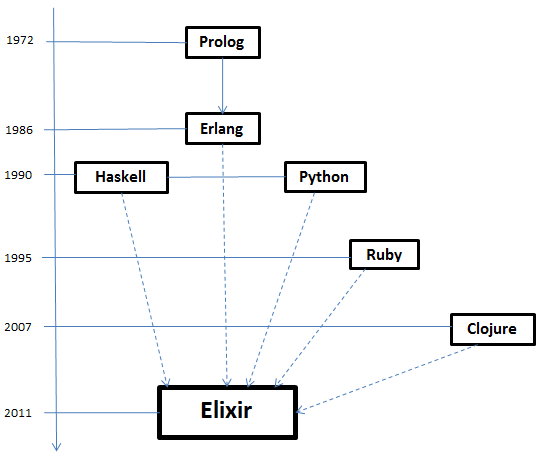
\includegraphics[width=\textwidth]{dijagram_uticaja_jezika.PNG}
  \caption{Razvojno stablo jezika Elixir}
  \label{fig:razvojnoStablo}
\end{figure}



\subsection{Erlang}
Firma Erikson je 1981. godine oformila novu laboratoriju \textbf{Erikson CSLab} (engl. \textit{The Ericsson CSLab}) sa ciljem da predlaže i stvara nove arhitekture, koncepte i strukture za buduće softverske sisteme \cite{ErlangBook2}. Jedan od zadataka novonastale laboratorije bio je dodavanje konkurentnih procesa u programski jezik \textbf{Prolog}\footnote{Prolog (engl. \textit{\textbf{PRO}gramming in \textbf{LOG}ic}) je deklarativan programski jezik namenjen rešavanju zadataka simboličke prirode. Prolog se temelji na teorijskom modelu logike prvog reda. Početkom 1970-ih godina \textbf{Alen Kolmerur} (engl. \textit{Alain Colmerauer}) i \textbf{Filip Rusel} (engl. \textit{Philippe Roussel}) na Univerzitetu u Marselju, zajedno sa \textbf{Robertom Kovalskim} (engl. \textit{Robert Kowalski}) sa Departmana veštačke inteligencije na Univerzitetu u Edinburgu , razvili su osnovni dizajn jezika Prolog.} i njegovo unapređivanje. Prolog predstavlja začetak novog programskog jezika koji je 1987. godine nazvan \textbf{Erlang}. Ime je nastalo zahvaljujući inicijativi zaposlenih koji su radili na telefonskim prekidačima, a za koje je jezik dizajniran. Naime, oni su predložili da jezik nosi ime Erlang u čast danskom matematičaru i inženjeru Agneru Krarupu Erlangu (engl. \textit{Agner Krarup Erlang}), a što je ujedno odgovaralo i skraćenici od  "\textbf{Er}icsson \textbf{Lang}uage". Erlang se smatrao dijalektom Prologa sve do 1990. godine, kada je postao potpuno samostalan programski jezik sa sopstvenom sintaksom. Međutim, zadržao je neke delove sintakse i koncepte iz Prologa (promenljive počinju velikim slovom, svaka funkcionalna celina se završava tačkom, poklapanje obrazaca (engl. \textit{pattern matching})).

Nakon mnogo godina rada nastajale su sve brže, bolje i stabilnije verzije jezika, kao i \textbf{standardna biblioteka OTP} (engl. \textit{The Open Telecom Platform}) \cite{OTP}. Od decembra 1998. godine, kada su postali deo slobodnog softvera (engl. \textit{open source software}), Erlang i OTP se mogu slobodno preuzeti sa zvaničnog sajta jezika Erlang \cite{OTP}. Erlang dobija široko prihvatanje pojavom višejezgarnih procesora i njihovog novog skalabilnog pristupa konkurentnosti. Erlang je funkcionalan jezik idealan za svaku situaciju u kojoj su paralelnost, tolerancija na greške i brz odziv neophodni \cite{ErlangBook}, te se koristi u velikom broju kompanija za razvoj njihovih glavnih softverskih rešenja (npr. Erikson (engl. \textit{Ericsson}), Motorola, Votsap (engl. \textit{WhatsApp}), Jahu (engl. \textit{Yahoo!}),
Fejsbuk (engl. \textit{Facebook})).

Elixir je preuzeo izmenjenu Erlangovu sintaksu i dopunjenu Erlangovu standardnu biblioteku. Pokreće se na vituelnoj mašini jezika Erlang, što znači da je nasledio i sve karakteristike Erlang platforme koja postoji već godinama i koja se pokazala pouzdanim rešenjem za skalabilne aplikacije.

\subsection{Python}
\textbf{Python} je interpretirani jezik opšte namene čiji tvorac je Gido van Rosum (engl. \textit{Guido van Rossum}) \cite{Python}. Krajem 1980-ih je koncipiran kao naslednik jezika \textbf{ABC} \cite{ABC}, a prvi put je objavljen 1991. godine. Filozofija dizajna jezika Python naglašava čitljivost koda. Njegove jezičke konstrukcije i objektno-orijentisani pristup imaju za cilj da pomognu programerima da napišu jasan i logičan k$\hat{o}$d za male i velike projekte. Python je dinamički tipiziran jezik i poseduje sistem za prikupljanje smeća (engl. \textit{garbage collector}). Podržava više paradigmi programiranja uključujući proceduralno, objektno-orijentisano i funkcionalno programiranje. Python interpreteri su dostupni za mnoge operativne sisteme. Globalna zajednica programera razvija i održava referentnu implementaciju otvorenog koda \textbf{CPython}. Neprofitna organizacija \textit{The Python Software Foundation} upravlja i usmerava resursima za razvoj jezika Python i CPython. Jedna od osobina koje je Elixir nasledio od Python-a je podrška za dokumentaciju u vidu dokumentacionih stringova (engl. \textit{docstrings}) koji omogućavaju povezivanje dokumentacije sa modulima, funkcijama, klasama, metodama.

\newpage

\subsection{Haskell}
\textbf{Haskell} je čisto funkcionalni jezik koji je statički tipiziran \cite{Haskell}. Nazvan je po Haskelu Bruks Kariju (engl. \textit{Haskell Brooks Curry}), čiji rad u oblasti matematičke logike služi kao osnova za sve funkcionalne jezike. Haskell je zasnovan na lambda računu, pa se stoga lambda koristi kao logo jezika. Nudi kratak, jasan i održiv k$\hat{o}$d, mali procenat grešaka i veliku pouzdanost. Stoga je pogodan za pisanje velikih softverskih sistema, jer njihovo održavanje čini lakšim i jeftinijim. Jedna od karakteristika koje je Elixir preuzeo od ovog jezika je lenjo izračunavanje.

\subsection{Ruby}
\textbf{Ruby} je dinamički tipiziran programski jezik otvorenog koda nastao 1995. godine. Kod ovog programskog jezika fokus je na jednostavnosti i produktivnosti. Ruby ima elegantnu sintaksu koja je prirodna za čitanje i lako pisanje.
Ruby je interpretirani programski jezik, što znači da se izvorni k$\hat{o}$d prevodi u k$\hat{o}$d razumljiv računaru prilikom svakog izvršavanja programa. Interpretirani programski jezici su sporiji od kompajliranih, ali su fleksibilniji i potrebno je kraće vreme za izradu programa.
Međutim, sve više iskusnih Ruby programera se okreće Elixir-u. Zapravo, Elixir je prvi jezik nakon Ruby-ja koji zaista brine o lepoti koda i korisničkom iskustvu vezanom za jezik, biblioteke i ekosistem. 

Ruby je imao veliki uticaj na sintaksu programskog jezika Elixir. Na slici \ref{fig:RubyElixirCode} se nalaze delovi koda napisani u jeziku Ruby i jeziku Elixir, koji imaju dosta sličnosti, a čiji je rezultat izvršavanja isti - dva stringa su nadovezana. U jeziku Ruby se definiše klasa \textit{Concat} koja ima polje \textit{value}, funkciju \textit{initialize} koja se poziva pri kreiranju objekta klase radi inicijalizacije polja \textit{value} i funkciju \textit{join} koja vrši nadovezivanje dva stringa. U Elixir-u se umesto klase definiše modul \textit{Concat} koji sadrži samo funkciju \textit{join} koja vrši nadovezivanje dva stringa. Uočavaju se sličnosti u sintaksi koje su ilustrovane ovim primerom pri definisanju klasa/modula, funkcija (ključne reči \textit{def} i \textit{end}), zatim pri nadovezivanju stringova (operatori $+$ i $<>$) i pozivanju funkcija (ime klase/modula za kojim sledi tačka).

\begin{figure}[!ht]
  \centering
  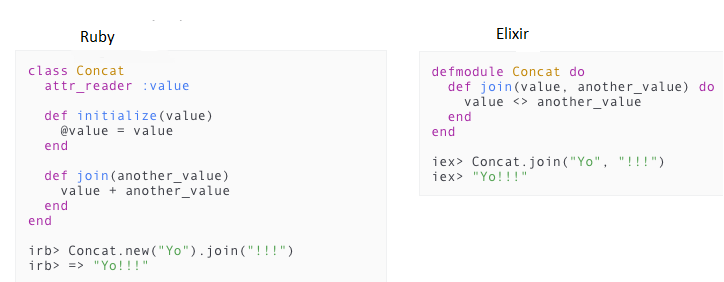
\includegraphics[width=\textwidth,height=6.5cm]{rubyVSelixir.png}
  \caption{K$\hat{o}$d za nadovezivanje dva stringa u jezicima Ruby i Elixir}
  \label{fig:RubyElixirCode}
\end{figure}

\subsection{Clojure}
\textbf{Clojure} je dinamički tipiziran programski jezik opšte namene nastao 2007. godine. Njegov tvorac je Rič Hiki (engl. \textit{Rich Hickey}). Clojure kombinuje pristupačnost i interaktivni razvoj skriptnog jezika sa efikasnom i robusnom infrastrukturom za višenitno programiranje. On je kompajlirani jezik, ali je i dalje potpuno dinamički tipiziran - svaka funkcija koju podržava Clojure je podržana u toku izvršavanja. Predstavlja dijalekt Lisp-a\footnote{Lisp je programski jezik  zasnovan na matematičkoj teoriji rekurzivnih funkcija
(u kojoj se funkcija pojavljuje u sopstvenoj definiciji), a Lisp program je funkcija
koja se primenjuje na podatke. Ime
LISP je nastalo od „LISt Processor”, a povezane liste su jedan od glavnih tipova
podataka. Osnova Lisp-a je funkcionalno programiranje, ali se Lisp zbog raznih drugih svojstava smatra multiparadigmatskim programskim jezikom.} i deli njegovu filozofiju \textit{code-as-data} (program je funkcija koja se izvršava nad podacima) i moćan makro sistem. Clojure je pretežno funkcionalni programski jezik i sadrži bogat skup nepromenljivih i postojanih struktura podataka. Elixir je preuzeo neke od najboljih Clojure karakteristika - efikasne, nepromenljive strukture podataka, opcionalno lenjo izračunavanje i protokole.


\section{Uputstvo za instalaciju i pokretanje Elixir-a}
\label{odeljak:Instalacija}

Za instaliranje Elixir-a je potrebno posetiti zvanični sajt jezika Elixir \cite{Elixir} i pratiti uputstva za odgovarajući operativni sistem. Kada se instalacija završi, može se proveriti verzija Elixir-a pomoću komande \textit{elixir --version} izvršene u komandnoj liniji.

Elixir programi imaju ekstenziju \textit{.ex} ili \textit{.exs} i mogu se pisati i izvršavati u okviru odgovarajućih integrisanih razvojnih okruženja. Neki od najpoznatijih su \textit{Spacemacs}, \textit{Visual Studio Code}, \textit{Emacs} i \textit{Atom}, a čitav spisak, kao i link ka njihovim zvaničnim stranicama, može se videti na adresi \cite{ElixirEditors}.

Pojedinačni izrazi, ali i Elixir programi, mogu se takođe izvršavati u komandnoj liniji nakon izvršavanja komande \textit{iex} i pokretanja interaktivnog Elixir-a. Primer pokretanja interaktivnog Elixir-a i izvršavanja pojedinačnog izraza može se videti na listingu \ref{lst:interactiveElixir}.

\lstinputlisting[language=erlang,label={lst:interactiveElixir},caption=Pokretanje interaktivnog Elixir-a,captionpos=b]{interactiveElixir.ex}

\noindent U Elixir-u se sve funkcije definišu u okviru modula pomoću ključne reči \textit{defmodule}. Za kompajliranje Elixir fajla u kome je definisan modul sa funkcijama i pokretanje interaktivnog Elixir-a nakon toga, najpre se poziva komanda \textit{iex imeFajla.ex}. Potom se može pokrenuti bilo koja funkcija unutar definisanog modula tako što se navede ime modula i ime funkcije razdvojeni tačkom, za kojima slede argumenti u okviru zagrada (\textit{imeModula.imePrograma(argument1, argument2)}). Primer definisanja modula i funkcije u okviru njega može se videti na listingu \ref{lst:printArgs}, a primer kompajliranja fajla i pokretanja funkcije dat je na listingu \ref{lst:primerPokretanjaHelloWorld}.

\lstinputlisting[language=erlang,label={lst:printArgs},caption=Primer definisanja modula,captionpos=b]{odstampaj_argumente.ex}

\lstinputlisting[language=erlang,label={lst:primerPokretanjaHelloWorld},caption=Primer kompajliranja fajla i pokretanja programa,captionpos=b]{primerPokretanjaHelloWorld.ex}

Elixir programi koji imaju ekstenziju \textit{.exs} se mogu kompajlirati i izvršavati iz komandne linije pomoću komande \textit{elixir imePrograma.exs}. Nakon ove komande neće biti pokrenut interaktivni Elixir, već će samo biti prikazani rezultati izvršavanja programa.

\section{Osnovne karakteristike}

Hosé Valim je tokom 2010. godine bio zaposlen u kompaniji \textit{Platformatec} \cite{Platformatec} i radio je na poboljšanju performansi okruženja
\textit{Ruby on Rails} na višejezgarnim sistemima. Shvatio je da Ruby nije bio dovoljno dobro dizajniran da reši problem konkurentnosti, pa je započeo istraživanje drugih tehnologija koje bi bile prihvatljivije. Tako je otkrio Erlang i upravo ga je interesovanje prema virtuelnoj mašini jezika Erlang podstaklo da započne pisanje jezika Elixir. Uticaj projekta na kome je do tada radio odrazio se na to da Elixir ima sintaksu koja je nalik na sintaksu jezika Ruby. Ovaj jezik se pokazao veoma dobro pri upravljanju
milionima simultanih konekcija: u 2015. je zabeleženo upravljanje nad dva miliona \textit{WebSocket} konekcija, dok je u 2017. za skalirani Elixir zabeležena obrada pet miliona istovremenih korisnika. Elixir se danas koristi u velikim kompanijama, kao što su \textit{Discord}  i \textit{Pinterest} \cite{HistoryOfElixir}.

Elixir je dinamički tipiziran, funkcionalni programski jezik koji se pokreće na vituelnoj mašini jezika Erlang, pa samim tim i nasleđuje pogodna svojstva koje dolaze sa ovim okruženjem kao što su \textbf{konkurentnost} i \textbf{tolerisanje grešaka} \cite{DefinicijaElixira}. Elixir je nadomestio mnoge koncepte koji su nedostajali jeziku Erlang. Neki od njih su  \textbf{metaprogramiranje}\footnote{Tehnika koja omogućava da programi posmatraju druge programe kao svoje podatke i na taj način čitaju i modifikuju i njihov i svoj k$\hat{o}$d u vreme izvršavanja.}, \textbf{polimorfizam}, \textbf{makroi} i \textbf{podrška za alate}. Elixir poseduje podrazumevano okruženje, takozvani \textbf{Kernel}, koji obezbeđuje podršku za osnovne tipove i funkcionalnosti jezika. 

U ovom delu će biti opisani osnovni tipovi jezika Elixir, njegove osobine, osnove njegove sintakse, semantike, kao i podrška za osnovne koncepte funkcionalnih jezika poput poklapanja obrazaca i nepromenljivosti podataka. 

\newpage

\section{Osnovni tipovi podataka}

Elixir ima svoje ugrađene (primitivne) tipove. To su: 
\begin{enumerate}
\itemsep0em 
    \item {Atomi}
    \item {Celi brojevi}
    \item {Brojevi u pokretnom zarezu}
    \item {Portovi}
    \item {Ugrađene torke}
    \item {Liste}
    \item {Mape}
    \item {Funkcije}
    \item {Niske bitova}
    \item {Reference}
\end{enumerate}

Svaki od ovih tipova, osim poslednja dva, ima odgovarajuće module koji sadrže funkcije koje se koriste za operacije nad tim tipom. Oni predstavljaju omotač oko primitivnog tipa koji nam omogućava korišćenje dodatnih funkcionalnosti nad njim. U nastavku će biti opisani neki od osnovnih tipova.

\subsubsection{Atomi}
Atomi su konstante ili simboli, pri čemu njihovo ime predstavlja njihovu vrednost. Počinju dvotačkom (:) i mogu sadržati slova, cifre, simbole \_, @. Mogu se završavati sa ! i ?. Atomi se mogu naći svuda u Elixir-u. U \textit{listama ključnih reči} koje će biti opisane u odeljku \ref{odeljak:ključneReči}, predstavljaju prvu vrednost elementa liste i često se koriste da označe uspeh (\textit{:ok}) ili grešku (\textit{:error}).

\subsubsection{Celi brojevi}
Celi brojevi u Elixir-u su predstavljeni slično kao i u većini programskih jezika i mogu biti dekadni, heksadekadni, oktalni i binarni. Karakter \_ se može koristiti za odvajanje blokova cifara. Veoma značajna stvar je da ne postoji fiksna veličina za čuvanje celih brojeva u memoriji, već interna reprezentacija raste kako bi broj mogao biti smešten u potpunosti.

\subsubsection{Brojevi u pokretnom zarezu}
Brojevi u pokretnom zarezu se zapisuju uz pomoć decimalne tačke po standardu \textit{IEEE 754}. Pre i posle decimalne tačke mora biti najmanje jedna cifra ($1.0$, $0.2456$). Može se koristiti i notacija koja obuhvata navođenje eksponenata ($0.314159e1$, $314159.0e-5$). 

\subsubsection{Liste}
Liste se čuvaju u memoriji kao povezane liste, što znači da svaki element u listi čuva svoju vrednost i ukazuje na sledeći element sve dok se ne dostigne kraj liste. To znači da je pristup proizvoljnom elementu liste kao i određivanje dužine liste linearna operacija, jer je potrebno da prođemo celu listu da bismo odredili njenu dužinu. Slično, performanse spajanja dve liste zavise od dužine one koja se nalazi sa leve strane, jer se spajanje vrši nadovezivanjem liste sa desne strane na kraj liste koja se nalazi sa leve strane. Da bi se izvršilo nadovezivanje, mora se odrediti dužina liste sa leve strane.

Elixir koristi uglaste zagrade $([\,\,])$ da označi listu vrednosti. Vrednosti mogu biti bilo kog tipa, a primer liste sa vrednostima različitih tipova prikazan je na listingu \ref{lst:prvi}.

\lstinputlisting[language=erlang,label={lst:prvi},caption=Primer liste,captionpos=b]{prvi.ex}

Nadovezivanje ili oduzimanje dve liste korišćenjem operatora $++/2$ i $--/2$ prikazano je na listingu \ref{lst:drugi}. Rezultat oduzimanja dve liste je nova lista koja nastaje tako što se iz liste sa leve strane operatora $--$ eliminišu elementi koji se nalaze u listi sa desne strane.

\lstinputlisting[language=erlang,label={lst:drugi},caption=Nadovezivanje i oduzimanje dve liste,captionpos=b]{drugi.ex}

Operatori za rad nad listama nikada ne menjaju postojeću listu. Rezultat povezivanja listi ili uklanjanja elemenata iz liste je uvek nova lista, jer su strukture podataka u Elixir-u nepromenljive. Jedna od prednosti nepromenljivosti je jasniji k$\hat{o}$d. Omogućeno je slobodno prosleđivanje podatka sa garancijom da neće biti izmenjeni u memoriji.

Lista može biti prazna ili se može sastojati od \textbf{glave} i \textbf{repa}. Glava je prvi element liste, a rep je ostatak liste. Oni se mogu izdvojiti pomoću funkcija \textit{hd/1} i \textit{tl/1}. Dodeljivanje liste promenljivoj, dohvatanje njene glave i repa prikazano je na listingu \ref{lst:treci}. Izdvajanje glave ili repa prazne liste rezultuje greškom.

\lstinputlisting[language=erlang,label={lst:treci},caption=Izdvajanje glave i repa liste,captionpos=b]{treci.ex}

Prilikom kreiranja liste, ukoliko Elixir vidi listu \textit{ASCII} brojeva, ispisaće listu znakova. Liste znakova su uobičajene kada se povezuju sa postojećim Erlang kodom. Primer koda koji ilustruje ovo prikazan je na listingu \ref{lst:cetvrti}.

\lstinputlisting[language=erlang,label={lst:cetvrti},caption=Lista vrednosti pod jednostrukim navodnicima,captionpos=b]{cetvrti.ex}

 

Preuzimanje informacija o tipu neke vrednosti može se izvršiti pomoću funkcije \textit{i/1} i može se videti na listingu \ref{lst:peti}.

\lstinputlisting[language=erlang,label={lst:peti},caption=Preuzimanje informacija o tipu vrednosti,captionpos=b]{peti.ex}

Reprezentacije sa jednostrukim i dvostrukim navodnicima u Elixir-u nisu ekvivalentne i predstavljaju različite tipove. Primer se može videti na listingu \ref{lst:sesti}.

\lstinputlisting[language=erlang,label={lst:sesti},caption=Dva različita tipa,captionpos=b]{sesti.ex}

\subsection{Torke}

Torke se u Elixir-u definišu pomoću vitičastih zagrada $\{\}$. Kao i liste, mogu sadržati vrednosti bilo kog tipa. Primer torke sa vrednostima različitih tipova i određivanjem njene dužine prikazan je na listingu \ref{lst:sedmi}.

\lstinputlisting[language=erlang,label={lst:sedmi},caption=Primer torke i određivanje njene dužine,captionpos=b]{sedmi.ex}

Torke su strukture fiksne dužine koje bi trebalo da sadrže svega nekoliko elemenata koji su zapisani u memoriji jedan za drugim. To znači da se pristup elementu torke ili određivanje dužine torke izvršava u konstantnom vremenu. Razlika u odnosu na liste je u semantici upotrebe. Liste se koriste kada se manipuliše kolekcijom, dok se torke, zbog brzine pristupa njihovim elementima, uglavnom koriste za smeštanje povratne vrednosti funkcije. Na primer, \textit{File.read/1} je funkcija koja se može koristiti za čitanje sadržaja fajla. Ako putanja do fajla postoji, povratna vrednost funkcije je torka sa prvim elementom koji je atom \textit{:ok} i drugim elementom koji je sadržaj datog fajla. U suprotnom, povratna vrednost funkcije će biti torka gde je prvi element atom \textit{:error}, a drugi element opis greške. Primer upotrebe ove funkcije može se videti na listingu \ref{lst:deseti}.

\lstinputlisting[language=erlang,label={lst:deseti},caption=Primer upotrebe funkcije \textit{File.read/1},captionpos=b]{deseti.ex}

Indeksi torke počinju od nule, a primer izdvajanja elementa sa indeksom 1 može se videti na listingu \ref{lst:osmi}.

\lstinputlisting[language=erlang,label={lst:osmi},caption=Izdvajanje elementa torke sa indeksom 1,captionpos=b]{osmi.ex}

Umetanje novog elementa na određeno mesto u torki vrši se pomoću funkcije $put\_elem/3$. Ona vraća novu torku, u kojoj je tekući element na zadatoj poziciji zamenjen novim elementom, dok originalna torka ostaje neizmenjena. Primer koda koji ilustruje upotrebu ove funkcije prikazan je na listingu \ref{lst:deveti}.

\lstinputlisting[language=erlang,label={lst:deveti},caption=Umetanje novog elementa u torku,captionpos=b]{deveti.ex}

Kao i liste, torke su takođe nepromenljive. Svaka operacija nad torkom vraća novu torku i nikada ne menja postojeću. Ova operacija, kao i operacija ažuriranja torke je skupa, jer zahteva kreiranje nove torke u memoriji. Ovo se odnosi samo na samu torku, a ne na njen sadržaj. Na primer, prilikom ažuriranja torke, svi unosi se dele između stare i nove torke, osim unosa koji je izmenjen. Drugim rečima, torke i liste u Elixir-u mogu da dele svoj sadržaj, što smanjuje količinu memorije koju jezik treba da zauzme. Ove karakteristike performansi diktiraju upotrebu struktura podataka. 

\subsection{Liste ključnih reči i mape}
\label{odeljak:ključneReči}
Elixir podržava asocijativne strukture podataka. Asocijativne strukture podataka su one koje su u stanju da pridruže određenu vrednost ili više vrednosti ključu. Dve glavne strukture među njima su \textbf{liste ključnih reči} i \textbf{mape}.

\subsubsection{Liste ključnih reči}
U mnogim funkcionalnim programskim jezicima uobičajeno je da se koristi lista dvočlanih torki za predstavljanje strukture podataka ključ - vrednost. Elixir takođe podržava ovakav način predstavljanja. Dodatno, lista torki gde je prvi element torke atom (tj. ključ) u Elixir-u se naziva \textbf{lista ključnih reči}. Obezbeđena je i posebna sintaksa za definisanje takvih lista: $[key: value]$. Primer oba načina definisanja prikazan je na listingu \ref{lst:11}.

\lstinputlisting[language=erlang,label={lst:11},caption=Primer liste ključnih reči,captionpos=b]{11.ex}

Kako su liste ključnih reči liste, nad njima možemo primenjivati sve operacije dostupne nad listama. Na primer, korišćenjem operatora ++ može se izvršiti dodavanje nove vrednosti listi ključnih reči. Primer koda koji ilustruje ovo dodavanje dat je na listingu \ref{lst:12}.

\lstinputlisting[language=erlang,label={lst:12},caption=Dodavanje nove vrednosti listi ključnih reči,captionpos=b]{12.ex}

Elementima liste ključnih reči se pristupa na način prikazan na listingu \ref{lst:13}.

\lstinputlisting[language=erlang,label={lst:13},caption=Pristup elementu liste ključnih reči,captionpos=b]{13.ex}

Liste ključnih reči su važne, jer imaju tri posebne karakteristike:
\begin{enumerate}
\itemsep0em 
\item{Ključevi moraju biti atomi.}
\item{Ključevi su uređeni, onako kako je navedeno od strane programera.}
\item{Ključevi se mogu ponavljati.}
\end{enumerate}

Elixir obezbeđuje modul koji omogućava manipulisanje listama ključnih reči. Liste ključnih reči su jednostavno liste, i kao takve pružaju iste karakteristike linearnih performansi kao i liste. Što je lista duža, više vremena će biti potrebno za pronalaženje ključa, prebrojavanje elemenata i tako dalje. Iz tog razloga, liste ključnih reči se u Elixir-u koriste uglavnom za prosleđivanje opcionih vrednosti. Za čuvanje mnogo elemenata ili garantovanje pojavljivanja jednog ključa sa maksimalno jednom vrednošću treba koristiti mape.
 
\subsubsection{Mape}
Mapa je kolekcija koja sadrži parove ključ : vrednost. Glavne razlike između liste parova ključ-vrednost i mape su u tome što mape ne dozvoljavaju ponavljanje ključeva (jer su to asocijativne strukture podataka) i što ključevi mogu biti proizvoljnog tipa. Mapa je veoma efikasna struktura podataka, naročito kada količina podataka raste. Ukoliko želimo da podaci u kolekciji ostanu baš u onom redosledu u kom smo ih naveli inicijalno, onda je bolje koristiti liste parova ključ : vrednost, jer mape ne prate nikakvo uređenje.

Mapa se definiše pomoću sintakse \%\{\} na način prikazan na listingu \ref{lst:14}.

\lstinputlisting[language=erlang,label={lst:14},caption=Primer mape i pristupa njenim elementima,captionpos=b]{14.ex}

Modul \textbf{Map} obezbeđuje razne funkcije za manipulaciju mapama, a neke od njih mogu se videti na listingu \ref{lst:17}.

\lstinputlisting[language=erlang,label={lst:17},caption=Neke od funkcija modula Map,captionpos=b]{17.ex}

Mape imaju sintaksu za ažuriranje vrednosti ključa prikazanu na listingu \ref{lst:18}

\lstinputlisting[language=erlang,label={lst:18},caption=Ažuriranje vrednosti ključa,captionpos=b]{18.ex}

\noindent Prethodno prikazana sintaksa zahteva da dati ključ postoji u mapi i ne može se koristiti za dodavanje novih ključeva. Na primer, korišćenje ove sintakse za ključ :c nije uspelo, jer ključ :c ne postoji u mapi.



Ukoliko su svi ključevi u mapi atomi, onda se radi pogodnosti može koristiti sintaksa ključnih reči data listingom \ref{lst:19}.

\lstinputlisting[language=erlang,label={lst:19},caption=Sintaksa ključnih reči,captionpos=b]{19.ex}

Još jedno zanimljivo svojstvo mapa je to što obezbeđuju sopstvenu sintaksu za pristup atomskim ključevima. Primer ove sintakse možemo videti na listingu \ref{lst:20}.

\lstinputlisting[language=erlang,label={lst:20},caption=Sintaksa za pristup atomskim ključevima,captionpos=b]{20.ex}

\noindent Programeri koji programiraju u Elixir-u pri radu sa mapama češće koriste \textit{map.field} sintaksu i poklapanje obrazaca nego funkcije iz modula Map, jer dovode do asertivnog stila programiranja.

Često se koriste mape unutar mapa ili čak liste ključnih reči unutar mapa. Elixir obezbeđuje pogodnosti za manipulisanje ugnježdenim strukturama podataka poput $put\_in/2$, $update\_in/2$ i drugih naredbi koje daju iste pogodnosti koje se mogu pronaći u imperativnim jezicima, a da pritom zadrže svojstvo nepromenljivosti podataka (svojstvo koje će detaljnije biti objašnjeno u poglavlju \ref{odeljak:nepromenljivostPodataka}).

Na listingu \ref{lst:21} je prikazana lista ključnih reči korisnika, gde je svaka vrednost mapa koja sadrži ime, starost i listu programskih jezika koje svaki korisnik voli.

\lstinputlisting[language=erlang,label={lst:21},caption=Struktura koja predstavlja listu korisnika,captionpos=b]{21.ex}

\noindent Pristup Džonijevim godinama mogao bi se izvršiti na način prikazan na listingu \ref{lst:22}.

\lstinputlisting[language=erlang,label={lst:22},caption=Pristup broju godina korisnika sa imenom Dzoni,captionpos=b]{22.ex}

\noindent Ista sintaksa se može koristiti i za ažuriranje vrednosti i prikazana je na listingu \ref{lst:23}.

\lstinputlisting[language=erlang,label={lst:23},caption=Ažuriranje vrednosti,captionpos=b]{23.ex}

Makro $update\_in/2$ je sličan, ali daje mogućnost prosleđivanja funkcije koja kontroliše kako se vrednost menja. Na primer, uklanjanje programskog jezika Clojure sa Marijinog spiska jezika može se uraditi na način prikazan listingom \ref{lst:24}.

\lstinputlisting[language=erlang,label={lst:24},caption=Brisanje jezika iz liste,captionpos=b]{24.ex}

Funkcija $get\_and\_update\_in$ omogućava pristup vrednosti i ažuriranje strukture podataka odjednom, a funkcije $put\_in/3$, $update\_in/3$ i $get\_and\_update\_in/3$ omogućavaju dinamički pristup strukturama podataka.



\section{Osnovni operatori}

Pored osnovnih artimetičkih operatora $+$, $-$, $*$, $/$, kao i funkcija \textit{div/2} i \textit{rem/2} za celobrojno deljenje i ostatak pri celobrojnom deljenju, Elixir podržava i već pomenute operatore $++$ i $--$ za nadovezivanje i oduzimanje listi, kao i operator $<>$ koji se koristi za nadovezivanje stringova.

Elixir obezbeđuje tri logička operatora: \textbf{and}, \textbf{or} i \textbf{not}. Oni su striktni u smislu da očekuju nešto što ima vrednost \textit{true} ili \textit{false} kao svoj prvi operand. Primer koda koji ilustruje ovu osobinu prikazan je na listingu \ref{lst:25}.

\lstinputlisting[language=erlang,label={lst:25},caption=Primer upotrebe logičkih operatora,captionpos=b]{25.ex}

\noindent Ukoliko kao prvi operand prosledimo nešto čija vrednost nije logička, rezultat je greška kao na listingu \ref{lst:26}.

\lstinputlisting[language=erlang,label={lst:26},caption=Greška pri upotrebi logičkog operatora,captionpos=b]{26.ex}

\noindent \textit{And} i \textit{or} su lenji operatori, jer desni operand izračunavaju samo u slučaju da levi nije dovoljan za određivanje rezultata.

Pored ovih logičkih operatora, Elixir takođe obezbeđuje operatore $||$, $\&\&$ i $!$ koji prihvataju argumente bilo kog tipa. Povratna vrednost ovih operatora ne mora biti logička, već može biti i brojevna. Sve vrednosti osim \textbf{false} i \textbf{nil} će biti procenjene na \textit{true}, što se može videti na primeru prikazanom listingom \ref{lst:27}.

\lstinputlisting[language=erlang,label={lst:27},caption=Operatori koji prihvataju argumente bilo kog tipa,captionpos=b]{27.ex}

Pravilo je da kada se očekuju logičke vrednosti, treba koristiti operatore \textit{and} i \textit{or}, a ako bilo koji od operanada ima vrednost koja nije logička, onda treba koristi $||$, $\&\&$ i $!$.

Elixir takođe obezbeđuje $==$, ${!}{=}$, $===$, ${!}{=}{=}$, $<=$, $>=$, $<$ i $>$ kao operatore poređenja, pri čemu se operator $===$ od operatora $==$ razlikuje po tome što pored vrednosti poredi i tip.

Moguće je i poređenje tipova među sobom. Razlog zbog kojeg se mogu uporediti različiti tipovi podataka je pragmatizam. Algoritmi sortiranja ne moraju da brinu o različitim tipovima podataka da bi sortirali. Ukupan redosled sortiranja je definisan na način prikazan na listingu \ref{lst:37}.

\lstinputlisting[language=erlang,label={lst:37},caption=Poređenje tipova,captionpos=b]{37.ex}

\section{Poklapanje obrazaca}

Poklapanje obrazaca je proveravanje da li se u datoj sekvenci tokena može prepoznati neki obrazac. Ovaj koncept će biti jasniji na praktičnom primeru operatora $=$. U većini programskih jezika, operator $=$ je operator dodele koji levoj strani dodeljuje vrednost izraza na desnoj. U Elixir-u se ovaj operator naziva \textbf{operator uparivanja} (engl. \textit{matching}). On se uspešno izvršava, ako pronađe način da izjednači levu stanu (svoj prvi operand) sa desnom (drugi operand).

Na primer, izraz $5 = 2 + 2$ bi rezultirao greškom datom na listingu \ref{lst:28}.

\lstinputlisting[language=erlang,label={lst:28},caption=Operator uparivanja,captionpos=b]{28.ex}

Na osnovu greške se može zaključiti da $2 + 2$ zaista nije 5. U Elixir-u leva strana mora da ima istu vrednost kao i desna strana. Vrednost izraza dat listingom \ref{lst:29} nije greška, već uspešno poklapanje obrazaca:

\lstinputlisting[language=erlang,label={lst:29},caption=Uspešno poklapanje obrazaca,captionpos=b]{29.ex}

Slično, dva identična stringa sa obe strane znaka jednakosti će dati rezultat prikazan listingom \ref{lst:30}.

\lstinputlisting[language=erlang,label={lst:30},caption=Uspešno poklapanje obrazaca sa stringovima,captionpos=b]{30.ex}

Poklapanje obrazaca se može prikazati i na primeru sa listama. Neka je data lista osoba koja je prikazana listingom \ref{lst:31}.

\lstinputlisting[language=erlang,label={lst:31},caption=Lista osoba,captionpos=b]{31.ex}

Neka prve tri osobe treba da budu zapamćene. U te svrhe se može iskoristiti poklapanje obrazaca dato na listingu \ref{lst:32}.

\lstinputlisting[language=erlang,label={lst:32},caption=Poklapanje obrazaca sa listama,captionpos=b]{32.ex}

Izvršeno je dodeljivanje prve, druge i treće stavke iz liste promenljivama \textit{prvi}, \textit{drugi} i \textit{treći}. Ostatak liste je dodeljen pomenljivoj \textit{ostali} pomoću \textbf{pipe operatora (|)}. Vrednost svake od ovih promenljivih može se iščitati na način prikazan na listingu \ref{lst:33}.

\lstinputlisting[language=erlang,label={lst:33},caption=Iščitavanje sadržaja promenljivih,captionpos=b]{33.ex}

Mape su vrlo korisne kod poklapanja obrazaca. Kada se koristi u poklapanju obrazaca, mapa će se uvek podudarati sa podskupom date vrednosti kao što se može videti na listingu \ref{lst:15}.
 
\lstinputlisting[language=erlang,label={lst:15},caption=Mape pri poklapanju obrazaca,captionpos=b]{15.ex}

\noindent Mapa se podudara sve dok ključevi u obrascu postoje u datoj mapi. Tako, prazna mapa odgovara svim mapama.

Promenljive se mogu koristiti prilikom pristupa, podudaranja i dodavanja ključeva mape, što je dato listingom \ref{lst:16}.

\lstinputlisting[language=erlang,label={lst:16},caption=Upotreba promenljivih u mapama,captionpos=b]{16.ex}

\section{Nepromenljivost podataka}
\label{odeljak:nepromenljivostPodataka}

U mnogim programskim jezicima je dozvoljeno dodeljivanje vrednosti promenljivoj, a zatim njeno menjanje tokom izvršavanja programa. Mogućnost zamene vrednost na određenoj memorijskoj lokaciji drugom vredošću čini se legitimna i čini se da povećava čitljivost našeg programa. Tokom izvršavanja programa obično se ne zna tačno vreme izvršavanja ove promene i obično se i ne vodi računa o tome pri pisanju programa. Ali šta se dešava kada se vrednost u memoriji, ili čak i tip vrednosti, promeni u trenutku kada je koristi više instanci programa?  Ovakvo ponašanje je poznato kao \textbf{promenljivost (mutabilnost)}. U konkurentnim okruženjima je izvor grešaka koje je veoma teško pratiti i reprodukovati. Promenljivost takođe vodi veoma komplikovanom kodu, koji se često piše ad-hoc kako bi se rešili problemi sinhronizacije.

Umesto toga, drugi jezici, kao što je Erlang, a samim tim i Elixir imaju osobinu \textbf{nepromenljivosti (imutabilnosti)}. Oni jednostavno ne dozvoljavaju promenu vrednosti na određenoj memorijskoj lokaciji. Na ovaj način, ako se promenljiva \textit{a} poklopila sa vrednošću 1, onda se njena vrednost sigurno neće menjati tokom izvršavanja programa i ne mora se voditi računa o problemima sinhronizacije u konkurentnom okruženju.

\section{Konkurentnost}

Jedna od glavnih karakteristika Elixir-a je ideja o organizovanju koda u male komande koje se mogu izvršavati nezavisno i istovremeno. Zahvaljujući arhitekturi virtuelne mašine Erlang-a na kojoj se Elixir pokreće, stvaranje velikog broja procesa ne utiče na smanjivanje performansi. Elixir koristi model konkurentnosti \textit{\textbf{actor}}. \textit{Actor} je nezavisan proces koji ne deli ništa sa bilo kojim drugim procesom. Mogu se stvarati novi procesi, slati poruke procesima i primati poruke od njih. Procesi u Elixir-u nemaju nikakve veze sa izvornim procesima operativnog sistema koji su spori i glomazni. Elixir koristi podršku za procese iz Erlang-a. Ovi procesi se odvijaju širom svih centralnih procesorskih jedinica, baš kao i izvorni procesi operativnog sistema, ali koriste vrlo malo resursa. Moguće je stvoriti stotine hiljade procesa čak i na skromnom računaru. Na listingu \ref{lst:proces} se nalazi k$\hat{o}$d koji definiše modul \textit{KreiranjeProcesa} i u okviru njega funkciju \textit{pozdrav} koja ispisuje \textit{Zdravo}.

\lstinputlisting[language=erlang,label={lst:proces},caption=Modul \textit{KreiranjeProcesa},captionpos=b]{proces.ex}

\noindent Nakon kompajliranja fajla u kome je definisan modul \textit{KreiranjeProcesa} pomoću komande \textit{iex ime\_fajla.ex}, na listingu \ref{lst:pokretanjeProcesa} se može videti regularno pokretanje funkcije \textit{pozdrav} i pokretanje u okviru posebnog procesa. Pokretanje u okviru posebnog procesa se vrši pomoću funkcije \textit{spawn}.

\lstinputlisting[language=erlang,label={lst:pokretanjeProcesa},caption=Pokretanje funkcije \textit{greet},captionpos=b]{pokretanje_procesa.ex}

Funkcija \textit{spawn} kreira novi proces. Pojavljuje se u mnogim oblicima, ali dva najjednostavnjija su ona koji omogućavaju pokretanje anonimne funkcije i pokretanje imenovane funkcije u modulu, prosleđujući listu argumenata. Drugi oblik je iskorišćen u primeru sa listinga \ref{lst:pokretanjeProcesa}. Ova funkcija vraća identifikator procesa koji se obično naziva \textit{\textbf{PID}} i koji jedinstveno identifikuje proces koji je kreiran. Kada se funkcija \textit{spawn} pozove, kreira se novi proces u okviru koga će se funkcija izvršiti. Ne zna se kada će tačno biti izvršena, ali se zna da je kvalifikovana za izvršavanje \cite{ProgrammingElixir}.

\section{Odlučivanje}

Strukture odlučivanja zahtevaju da programer odredi jedan ili više uslova koje će program proceniti ili testirati zajedno sa naredbom ili naredbama koje treba izvršiti, ako je uslov određen ili tačan, i opciono, druge naredbe koje treba izvršiti, ako je utvrđeno da je uslov netačan.

Elixir obezbeđuje \textbf{\textit{if/else}} uslovne konstrukte kao i mnogi drugi programski jezici. On takođe poseduje naredbu \textbf{\textit{cond}} koja poziva prvu tačnu vrednost koju pronađe. \textbf{\textit{Case}} je još jedan kontrolni tok koji koristi poklapanje obrazaca za kontrolu toka programa.

Elixir ima sledeće vrste naredbi za odlučivanje:

\begin{enumerate}
\itemsep0em 
    \item{\textit{if} - Naredba \textit{if} se sastoji od logičkog izraza praćenog ključnom reči \textit{do}, jedne ili više izvršnih naredbi i na kraju ključne reči \textit{end}}
    \item{\textit{if..else} - Naredba \textit{if} može biti praćena naredbom \textit{else} (unutar \textit{do..end} bloka), koja se izvršava, ako je logički izraz netačan.}
    \item{\textit{unless} - Naredba \textit{unless} ima isto telo kao i naredba \textit{if}. K$\hat{o}$d unutar \textit{unless} naredbe se izvršava samo kada je navedeni uslov netačan.}
    \item{\textit{unless..else} - Naredba \textit{unless...else} ima isto telo kao i naredba \textit{if..else}. K$\hat{o}$d unutar \textit{unless..else} naredbe se izvršava samo kada je navedeni uslov netačan.}
    \item{\textit{cond} - Naredba \textit{cond} se koristi ukoliko treba izvršiti neki k$\hat{o}$d na osnovu nekoliko uslova. Radi kao \textit{if..else} \textit{if..else} kod drugih programskih jezika.}
    \item{\textit{case} - Naredba \textit{case}  se može smatrati zamenom za naredbu \textbf{\textit{switch}} u imperativnim programskim jezicima. Naredba \textit{case} uzima promenljivu ili literal i primenjuje odgovarajući obrazac poklapanja u različitim slučajevima. Ako se bilo koji slučaj poklapa, Elixir izvršava k$\hat{o}$d povezan sa tim slučajem i izlazi iz naredbe \textit{case}.}
\end{enumerate}

\section{Moduli}

U Elixir-u se može vršiti grupisanje nekoliko funkcija u module. Već su pomenuti različiti moduli u prethodnim odeljcima (\textit{Map}, \textit{Enum}, \textit{List}, \textit{String},...). Za kreiranje sopstvenih modula u Elixir-u, koristi se makro \textbf{\textit{defmodule}}, a za definisanje svojih funkcija, koristimo makro \textbf{\textit{def}}. Primer koda koji ilustruje kreiranje modula i funkcija dat je listingom \ref{lst:34}.

\lstinputlisting[language=erlang,label={lst:34},caption=Kreiranje modula i funkcija,captionpos=b]{34.ex}

Moduli mogu biti ugnježdeni u Elixir-u. Ova osobina jezika omogućava bolje organizovanje koda. Na listingu \ref{lst:35} se može videti definisanje dva modula: \textbf{Matematika} i \textbf{Matematika.Sabiranje}, pri čemu je drugi ugnježden unutar prvog. Drugom se može pristupati samo pomoću \textit{Sabiranje} unutar modula \textit{Matematika} sve dok su u istom leksičkom opsegu. Ako se kasnije modul \textit{Sabiranje} premesti izvan definicije modula \textit{Matematika}, onda se mora referencirati njegovim punim imenom \textit{Matematika.Sabiranje} ili pseudonim mora biti postavljen pomoću direktive aliasa.

\newpage

\lstinputlisting[language=erlang,label={lst:35},caption=Ugnježdavanje modula,captionpos=b]{35.ex}

\noindent U Elixir-u nema potrebe za definisanjem modula \textit{Matematika}, kako bi se definisao modul \textit{Matematika.Sabiranje}, pošto jezik prevodi sva imena modula u atome. Mogu se  definisati i proizvoljno ugnježdeni moduli bez definisanja bilo kog modula u lancu. Na primer, može se definisati modul \textit{Matematika.Sabiranje.Saberi}, iako  prethodno nije definisan modul \textit{Matematika} i \textit{Matematika.Sabiranje}.

\section{Direktive}

Kako bi se olakšala ponovna upotreba koda, Elixir obezbeđuje tri direktive - \textbf{alias, require i import}, kao i makro \textbf{use}. Primer njihove upotrebe može se videti na listingu \ref{lst:36}.

\lstinputlisting[language=python,label={lst:36},caption=Primer upotrebe direktiva,captionpos=b]{36.ex}

\subsection{Direktiva \textit{alias}}
Direktiva aliasa služi za podešavanje pseudonima za bilo koje ime modula. Aliasi moraju uvek počinjati velikim slovom. Validni su samo unutar leksičkog opsega u kome su pozvani.

\subsection{Direktiva \textit{require}}
Elixir obezbeđuje makroe kao mehanizam za meta-programiranje (pisanje koda koji generiše k$\hat{o}$d). Makroi su delovi koda koji se izvršavaju i proširuju tokom kompilacije. To znači da bi se mogao koristiti makro, mora se garantovati da su njegovi moduli i implementacija dostupni tokom kompilacije. Ovo se čini pomoću \textbf{require} direktive. Uopšteno, moduli nisu potrebni pre upotrebe, osim ako želimo da koristimo makroe koji su dostupni u njemu. Require direktiva je takođe leksički određena.

\subsection{Direktiva \textit{import}}
Direktiva \textbf{import} se koristi kako bi se lakše pristupalo funkcijama i makroima iz drugih modula bez upotrebe potpuno kvalifikovanog imena. Import direktiva je takođe leksički određena. 

\subsection{Makro \textit{use}}
Iako nije direktiva, \textbf{use} je makro koji je usko povezan sa zahtevom koji omogućava korišćenje modula u trenutnom kontekstu. Makro use se često koristi za unos spoljne funkcionalnosti u trenutni leksički opseg, često modula.

% ------------------------------------------------------------------------------
%\chapter{Razrada}
%\label{chp:razrada}

\chapter{Sekvencioniranje genoma}
\label{poglavlje:Bio}

\begin{comment}
Posle prve rečenice da li ubaciti?
Sva živa bića svoj genetički materijal nose u obliku DNK, sa izuzetkom nekih virusa koji imaju ribonukleinsku kiselinu (RNK).\end{comment}

\textbf{DNK} (dezoksiribonukleinska kiselina) je nukleinska kiselina koja sadrži uputstva za razvoj i pravilno funkcionisanje svih živih organizama. Informacije u DNK se čuvaju kao k$\hat{o}$d koji čine \textbf{četiri azotne baze}: \textbf{adenin} (A), \textbf{guanin} (G), \textbf{citozin} (C) i \textbf{timin} (T). Ljudski DNK se sastoji od oko tri milijarde baza, a više od 99 procenata tih baza je isto kod svih ljudi. Redosled ili sekvenca ovih baza određuje informacije dostupne za izgradnju i održavanje organizma, slično načinu na koji se slova abecede pojavljuju određenim redosledom kako bi se formirale reči i rečenice. DNK baze se spajaju jedna sa drugom, adenin sa timinom i citozin sa guaninom, da bi formirale jedinice koje se nazivaju \textbf{bazni parovi}. Svaka baza je takođe vezana za molekul šećera dezoksiriboze i molekul fosfata. Zajedno, baza, šećer i fosfat nazivaju se \textbf{nukleotidima}. Nukleotidi su raspoređeni u dva dugačka lanca koji koja čine spiralu koja se naziva \textbf{dvostruka spirala} \cite{DNA}. Struktura dvostruke spirale pomalo je nalik na merdevine, pri čemu bazni parovi formiraju lestvičaste trake, a molekuli šećera i fosfata formiraju vertikalne bočne delove merdevina (slika \ref{fig:00}). Molekul DNK se može zamisliti odmotan i rotiran, tako da su trake merdevina orijentisane vertikalno, a bazni parovi se mogu čitati sa leva na desno (slika \ref{fig:odmotanDnk}).

\begin{figure}[!ht]
  \centering
  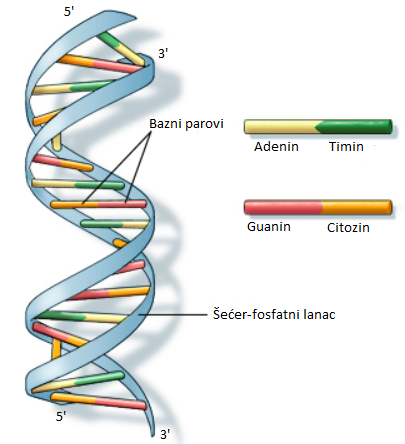
\includegraphics[width=0.7\textwidth]{dnk.PNG}
  \caption{Struktura DNK \cite{DNA}}
  \label{fig:00}
\end{figure}

\begin{figure}[!ht]
  \centering
  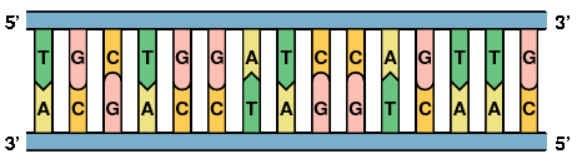
\includegraphics[width=0.7\textwidth]{odmotanDnk.PNG}
  \caption{Odmotan DNK \cite{DNA2}}
  \label{fig:odmotanDnk}
\end{figure}

\begin{comment}
 Šećeri u DNK su međusobno povezani fosfatnim grupama koje stvaraju fosfodiestarsku vezu između trećeg i petog ugljenikovog atoma šećernog prstena. Fosfodiestarske veze su asimetrične, te DNK polinukleotidni lanci imaju smer. Kako ovi lanci idu u suprotnim smerovima, kaže se da je DNK antiparalelna. Asimetrični krajevi DNK baza se označavaju sa 5' (pet prim) i 3' (tri prim). Antiparalelnost znači da jedan lanac ide u smeru 5' \rightarrow 3', dok suprotni lanac ide u smeru 3' \rightarrow 5'. 

$5'$ i $3'$ označavaju brojeve ugljenika koji se nalaze u osnovi DNK šećera. $5'$ ugljenik ima fosfatnu grupu koja je vezana za njega, a $3'$ ugljenik-hidroksilnu (-OH) grupu. Ova asimetrija daje DNK pravac koji se obeležava sa $5' \rightarrow 3'$. Na primer, DNK polimeraza deluje u pravcu $5' \rightarrow 3'$, tj. dodaje nukleotide na $3'$ kraj molekula napredujući u tom smeru.

\end{comment}

Krajevi šećer-fosfatnih lanaca se međusobno razlikuju po prirodi nevezanog atoma ugljenika - jedan kraj ima nevezani $5'$ (pet prim) atom ugljenika, dok drugi kraj ima nevezani $3'$ (tri prim) atom ugljenika. $5'$ ugljenik ima fosfatnu grupu koja je vezana za njega, a $3'$ ugljenik-hidroksilnu (-OH) grupu. Ova asimetrija daje DNK pravac $5' \rightarrow 3'$. Kada predstavljamo molekul DNK pomoću dijagrama, kakav je prikazan na slici \ref{fig:00}, podrazumeva se da gornji lanac kreće od $5'$ kraja sa leve strane do $3'$ kraja sa desne strane. Donji lanac je obrnuto orijentisan, od $3'$ kraja sa leve strane do $5'$ kraja sa desne strane \cite{DNA2}. 

Sva živa bića svoj genetički materijal nose u obliku DNK, sa izuzetkom nekih virusa koji imaju ribonukleinsku kiselinu (RNK). DNK ima veoma važnu ulogu ne samo u prenosu genetskih informacija sa jedne na drugu generaciju, već sadrži i uputstva za građenje neophodnih ćelijskih organela, proteina i RNK molekula. \textbf{Geni} su delovi DNK sekvence unutar kojih je kodirano pravilo za sintezu jednog proteina u ćeliji, koji je neophodan za njeno pravilno funkcionisanje. \textbf{Genom} je skup gena jednog organizma i sastoji od niza uparenih baza. Sa računarske strane genom predstavlja nisku nad azbukom $\{A, C, G, T\}$. Nukleotidi su raspoređeni u dva dugačka lanca koji imaju antiparalelnu\footnote{U biohemiji, dva molekula su antiparalelna, ako se prostiru paralelno, ali u suprotnim smerovima.} orijentaciju.

\textbf{Sekvencioniranje genoma} podrazumeva otkrivanje sastava genoma. U pitanju je veoma kompleksan proces koji uključuje i eksperimentalan deo – da bi se saznalo šta se nalazi u sastavu jednog genoma, potreban je uzorak tkiva
odgovarajuće vrste \cite{skriptaBio}. \textbf{Sekvencioniranje DNK} je proces određivanja preciznog redosleda nukleotida unutar molekula DNK, a mašine u kojima taj proces započinje se nazivaju \textbf{sekvenceri}. Sekvenceri za dati uzorak bilo kog tkiva bilo kog organizma (npr. krvi kod čoveka, dlake kod miša,...) mogu da očitaju podsekvence DNK koje se nazivaju \textbf{očitavanja} (engl. \textit{reads}), a koje je nakon toga neophodno sastaviti u polaznu DNK sekvencu pomoću posebnih alata za sklapanje, takozvanih \textbf{asemblera}. Podniske očitavanja dužine $k$ nazivaju se \textbf{k-meri}. Dužina genoma i dužina očitavanja DNK se mere u \textbf{baznim parovima (bp)}. Očitavanja mogu biti  \textbf{kratka} i \textbf{duga}. Kratka očitavanja imaju dužinu od 50 bp do 400 bp, a duga očitavanja dužinu veću od 400 bp.

Rekonstrukcija genoma kroz sekvencioniranje DNK je veoma važan problem. Ona se može uporediti sa kompletiranjem slagalice, gde su očitavanja delovi slagalice. Za razliku od kompletiranja slagalice, gde je poznata slika koju treba na kraju dobiti, pri rekonstrukciji genoma nije pozanto kako treba da izgleda krajnji rezultat. Što su delovi veći, slagalicu je lakše sastaviti. Zadatak asemblera je da na osnovu očitavanja, za koje ne postoji informacija sa kog dela genoma potiču, složi genomsku slagalicu.

\begin{comment}
Rekonstrukcija genoma kroz sekvencioniranje DNK je veoma važan problem u genomici. Postojeće biotehnologije ne mogu proći kroz ceo hromozom, jer je predugačak. Umesto toga, genom se rekonstruiše indirektno. Prvo, vrši se razbijanje genoma na DNK fragmente koristeći pristup očitavanja celog sekvencioniranog genoma (engl. \textit{whole genome shotgun approach}). Zatim se pomoću mašine za sekvencioniranje na osnovu fragmenata vrši dekodiranje DNK sekvence. Ove DNK sekvence se nazivaju \textbf{očitavanja (engl. \textit{reads})}. Usled slučajnog uzorkovanja , ekstahovana očitavanja pokrivaju ceo genom ravnomerno. Lepljenjem ovih očitavanja možemo računski rekonstruisati genom. Ovaj proces je poznat kao \textbf{genomsko sekvencioniranje \textit{de novo}}.
\end{comment}

\section{Istorija sekvencioniranja genoma}

\textbf{Sekvencioniranje Sanger} predstavlja prvu tehniku sekvencioniranja. Nastala je 1977. godine, a njeni tvorci su Frederik Sanger (engl. \textit{Frederick Sanger}) i njegove kolege. Razvijena su dva asemblera za asembliranje očitavanja sekvencioniranja Sanger: \textit{OLC}\footnote{Skraćenica od \textit{overlap layout consensus} (\textit{overlap} - izgradnja grafa preklapanja,
\textit{layout} - spajanje putanja u grafu u kontige, \textit{consensus} - određivanje najverovatnije sekvence
nukleotida za svaku kontigu.} asembler \textbf{Celera} i asembler \textbf{Ojler} zasnovan na De Brojnovim grafovima. \textbf{Humani referentni genom} sastavljen je korišćenjem ova dva pristupa. Humani referentni genom predstavlja reprezentativni primer skupa gena čoveka koje su prikupili naučnici. Kako su često sastavljeni sekvencioniranjem DNK većeg broja davalaca, referentni genomi ne predstavljaju skup gena nijedne pojedinačne osobe. Humani referentni genom \textit{\textbf{GRCh37}} \textit{(The Genome Reference Consortium human genome (build 37)}) je izveden 2009. godine iz DNK trinaest anonimnih dobrovoljaca iz države Bafalo u SAD. Referentni genomi se obično koriste kao uputstvo na osnovu koga se grade novi genomi, što im omogućava da se sastave mnogo brže i ekonomičnije. Međutim, kako je sekvencioniranje Sanger niskopropusno (omogućava sekvencioniranje malog broja očitavanja odjednom) i neekonomično, samo nekoliko genoma je sastavljeno pomoću njega.

Razvoj tehnika za sekvencioniranje \textbf{druge generacije} značajno je doprineo efikasnijem i ekonomičnijem sekvencioniraranju stotine miliona očitavanja. Međutim, očitavanja druge generacije sekvencioniranja su kratka. Njihova pojava je dovela do većeg broja uspešnih \textbf{\textit{de novo}} asemblerskih\footnote{\textit{De novo} asembleri su programi
koji vrše sklapanje tako što proširuju kratka očitavanja spajanjem susednih
očitavanja u dužu sekvencu, bez korišćenja referentne sekvence.} projekata, uključujući rekonstrukciju genoma \textbf{Džejmsa Votsona} (engl. \textit{James Watson}) i genoma \textbf{panda}. Iako je ovaj pristup ekonomičan, rezultat su bili fragmentisani genomi, jer su očitavanja kratka i ponavljajući regioni, takozvani \textbf{ponovci}, dugi. Ponovci su fenomen kada se šablon od nekoliko nukleotida pojavljuje više puta u nizu.

Od nedavno su na raspolaganju tehnike za sekvencioniranje \textbf{treće generacije}, koje proizvode duga očitavanja (dužine od oko 10000 bp). Duga očitavanja mogu obuhvatiti složene genomske karakteristike, omogućavajući njihovo ispravnije postavljanje u rekonstruisanom genomu, tj. mogu rešiti problem ponavljajućih regiona. Međutim, duga očitavanja imaju visoku stopu greške $(15\%-18\%)$. U cilju rešavanja ovog problema razvijen je veliki broj računskih metoda za korekciju grešaka u očitavanjima treće generacije sekvencioniranja.

\section{Sekvencioniranje \textit{shotgun} celokupnog genoma}

Jedna od tehnika druge generacije sekvencioniranja je  sekvencioniranje \textit{shotgun} celokupnog genoma. Prvi korak u ovom procesu je razbijanje genoma na skup očitavanja, a na osnovu njegovog uzorka. Postoje tri vrste očitavanja:

\begin{itemize}
\itemsep0em 
    \item {jednostrana očitavanja (engl. \textit{single-end reads})}
    \item {uparena očitavanja (engl. \textit{paired-end reads})}
    \item{partner-uparena očitavanja} (engl. \textit{mate-pair reads})
\end{itemize}

Jednostrana očitavanja su očitavanja koja se generišu tako što sekvencer čita DNK fragment samo u jednom smeru, ili sa $5'$, ili sa $3'$ kraja. U slučaju uparenih očitavanja, sekvencer čita DNK fragment sa oba kraja. Partner-uparena očitavanja su $5'$ ili $3'$ očitavanja DNK fragmenta oba lanca. Prikaz ovih vrsta očitavanja može se videti na slici \ref{fig:01}. Strelice označavaju smer u kome je sekvencer vršio očitavanje DNK fragmenta.

\begin{figure}[!ht]
  \centering
  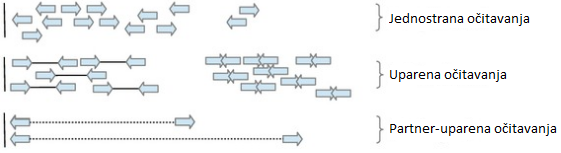
\includegraphics[width=\textwidth]{vrste_ocitavanja.PNG}
  \caption{Vrste očitavanja \cite{wholeGenomeSeq}}
  \label{fig:01}
\end{figure}

Sekvenceri čitaju deo DNK fragmenta neke unapred
zadate dužine koja se naziva \textbf{dužina očitavanja}. \textbf{Dubina pokrivanja} neke pozicije u DNK sekvenci je velika, ako je nukleotid na toj poziciji pročitan veliki broj puta u jedinstvenim očitavanjima. Tačnost sekvencioniranja za svaki pojedinačni nukleotid je veoma visoka, ali ukoliko se pojedinačni genom sekvencira samo jednom, zbog veoma velikog broja nukleotida u genomu, doći ́će do značajnog broja grešaka u sekvencioniranju. Pored toga, neke pozicije u genomu sadrže retke \textbf{jednonukleotidne polimorfizme}\footnote{Pojava zamene mesta jednog nukleotida nekim drugim nukleotidom.} (engl. \textit{single-nucleotide polymorphisms - SNPs}). Stoga, kako bi se napravila razlika između grešaka u sekvencioniranju i pravih \textit{SNP}-ova, potrebno je još više poveć́ati tačnost sekvencioniranjem pojedinačnih genoma veći broj puta \cite{SequencingCoverage}.

Za potrebe sekvencioniranja \textit{shotgun} celokupnog genoma postoje dva protokola:
\begin{itemize}
\itemsep0em 
    \item {sekvencioniranje celokupnog genoma}
    \item {sekvencioniranje partner-uparenih očitavanja}
\end{itemize}

\noindent U okviru oba protokola prvo se uzorak genoma na slučajan način razbija na DNK fragmente, a potom se vrši odabir dužine očitavanja i izdvajanje fragmenata te dužine.

\subsection{Sekvencioniranje celokupnog genoma}

Nakon izdvajanja fragmenata DNK određene dužine, vrši se sekvencioniranje jednostranih očitavanja ili sekvencioniranje uparenih očitavanja. Pri sekvencioniranju jednostranih očitavanja, sekvencer čita DNK fragment u jednom smeru, dok u slučaju uparenih očitavanja, fragment biva pročitan u oba smera. Pomenuti koraci su prikazani na slici \ref{fig:1}.

\begin{figure}[!ht]
  \centering
  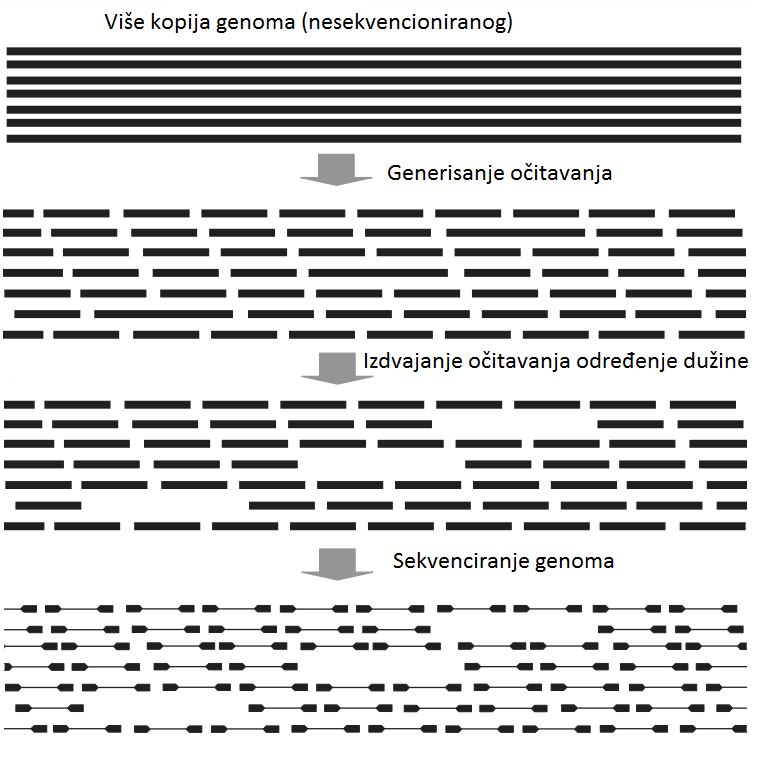
\includegraphics[width=0.7\textwidth]{prva.png}
  \caption{Sekvencioniranje \textit{shotgun} celokupnog genoma \cite{WingKinSung}}
\label{fig:1}
\end{figure}

Na slici \ref{fig:2} prikazan je odmotan i rotiran DNK fragment. Delovi koji se nalaze na poziciji koja premašuje dužinu očitavanja i ne ulaze u sastav očitavanja označeni su sa $N$. 

\begin{figure}[!ht]
  \centering
  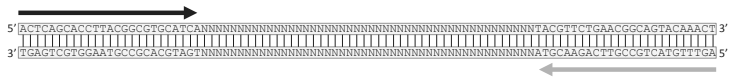
\includegraphics[width=\textwidth, height=2.4cm]{druga.PNG}
  \caption{DNK fragment ekstrahovan iz uzorka genoma \cite{WingKinSung}}
  \label{fig:2}
\end{figure}

 Prilikom sekvencioniranja jednostranih očitavanja, dobija se očitavanje sa $5'$ kraja gornjeg lanca, tj. $ACTCAGCACCTTACGGCGTGCATCA$. Prilikom sekvencioniranja uparenih očitavanja, dobijaju se $5'$ očitavanja i gornjeg i donjeg lanca:

\begin{itemize}
\itemsep0em 
    \item {$ACTCAGCACCTTACGGCGTGCATCA$}
    \item {$AGTTTGTACTGCCGTTCAGAACGTA$}
\end{itemize}

\noindent Drugo očitavanje $AGTTTGTACTGCCGTTCAGAACGTA$ je obrnuti komplement očitavanja $TACGTTCTGAACGGCAGTACAAACT$, jer je drugo očitavanje dobijeno iz donjeg lanca koji je komplementaran sa gornjim.

Za asembliranje genoma, dužina očitavanja je veoma važan parametar. Različite tehnologije sekvencioniranja imaju različita ograničenja na dužinu očitavanja. Na primer, \textit{Illumina Hi-seq}\footnote{Illumina je američka kompanija koja je proizvodila visokopropusne sekvencere (omogućavaju sekvencioniranje velikog broja očitavanja odjednom  (engl. \textit{high-throughput sequencers})).} sekvencioniranje može izvršiti samo sekvencioniranje uparenih očitavanja dužine manje od 1000 bp. Za treću generaciju sekvencioniranja, ograničenje dužine očitavanja može biti veće od 10000 bp.


\subsection{Sekvencioniranje partner-uparenih očitavanja}

Sekvenceri druge generacije mogu izdvojiti partner-uparena očitavanja sa oba kraja kratkih fragmenata DNK (dužine očitavanja manje od 1000 bp). Za izdvajanje ovakvih očitavanja može se koristiti \textbf{sekvencioniranje partner-uparenih očitavanja}.

Sekvenceri prvo izdvajaju duge DNK fragmente neke fiksirane dužine očitavanja (npr. 10000 bp). Potom dodaju takozvane \textbf{adapter sekvence}\footnote{Adapter sekvence su kratke hemijski sintetizovane sekvence
nukleotida koje se mogu vezati za krajeve nepoznatih DNK sekvenci i neophodne
su u nekim koracima sekvenciranja.}
na krajeve svakog fragmenta (slika \ref{fig:3}(a)). Zatim se vrši sečenje fragmenta levo i desno od adapter sekvence (slika \ref{fig:3}(b)). Na kraju se uparena očitavanja ekstrahuju sekvencioniranjem uparenih očitavanja (slika \ref{fig:3}(c)).

%Slika 2.3 i opis Figure 5.3 iz knjige
\begin{figure}[!ht]
  \centering
  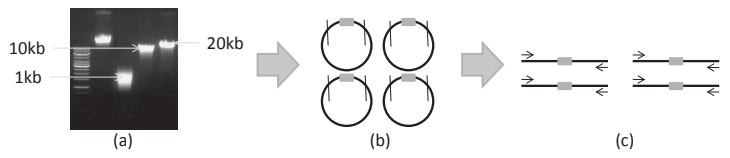
\includegraphics[width=0.8\textwidth, height=3cm]{treca.PNG}
  \caption{Sekvencioniranje partner-uparenih očitavanja \cite{WingKinSung}}
\label{fig:3}
\end{figure}

Orijentacije uparenih očitavanja očitanih od strane sekvencera partner-uparenog i uparenog očitavanja se razlikuju. Sekvenceri partner-uparenih očitavanja daju dva očitavanja sa oba kraja svakog fragmenta DNK u spoljašnjoj orijentaciji umesto u unutrašnjoj. Npr. za DNK fragment sa slike \ref{fig:2} sekvencioniranje partner-uparenih očitavanja će dati:
\begin{itemize}
\itemsep0em 
    \item {TGATGCACGCCGTAAGGTGCTGAGT}
    \item {TACGTTCTGAACGGCAGTACAAACT}
\end{itemize}

Iako protokol za sekvencioniranje partner-uparenih očitavanja može izdvojiti uparena očitavanja velike dužine očitavanja, on zahteva veći broj ulaznih kopija genoma za pripremu sekvencerskih biblioteka i sklon je greškama pri preklapanju očitavanja (engl. \textit{ligation errors}).
\begin{comment}
(ligation errors - greškama prilikom preklapanja očitavanja)
\end{comment}

% \section{Sekvencioniranje \textit{de novo} genoma za kratka očitavanja}

\section{Asembliranje \textit{de novo} genoma za kratka očitavanja}

Druga generacija tehnika sekvencioniranja omogućava dobijanje skupa jednostranih ili uparenih kratkih očitavanja celokupnog genoma. Asembliranje \textit{de novo} ima za cilj da izvrši preklapanje očitavanja u ispravnom redosledu i rekonstruiše genom.

Problem asembliranja genoma je računski težak. Čak i kada ne postoji greška sekvencioniranja, ovaj problem je ekvivalentan \textbf{problemu superstringa} za koji se zna da je NP-kompletan \cite{NPcomplexity}. Problem superstringa predstavlja problem pronalaženja superstringa na osnovu skupa stringova $S$, gde je superstring najkraći string $P$ takav da je svaki string $s$ iz skupa $S$ podstring stringa $P$. Na primer, ako je $S = \{ACATGC, ATGCGTGT, GTGTACGT\}$, onda je odgovarajući superstring $ACATGCGTGTACGT$.

Postoji veliki broj \textit{de novo} asemblera za asembliranje kratkih očitavanja. Opšte rešenje uključuje četiri koraka. U prvom koraku se koriguju greške u očitavanjima (opisano u poglavlju \ref{poglavlje:korekcijaGresaka}). Na osnovu korigovanih očitavanja, u drugom koraku se vrši spajanje očitavanja preklapanjem (opisano u poglavlju \ref{poglavlje:KonstrukcijaKontiga}). U idealnom slučaju, teži se spajanju svih očitavanja tako da se formira kompletan genom, ali kako se zbog ponovaka javljaju dvosmislenosti, to nije moguće. Postojeće metode, radi razrešavanja dvosmislenosti, preklapanjem očitavanja prvo grade kontinuirane sekvence, takozvane \textbf{kontige} (engl. \textit{contigs}). Kontige obično predstavljaju jednu \textbf{konsenzus nisku}\footnote{Niska sastavljena od najfrekventnijih nukleotida na pozicijama poravnatih sekvenci.}. Algoritmi za konstrukciju kontiga biće obrađeni u poglavlju \ref{poglavlje:KonstrukcijaKontiga}. Zatim, koristeći uparena očitavanja, vrši se rekonstrukcija redosleda kontiga tako da se formiraju \textbf{skafoldi} (engl. \textit{scaffolds}). Svaki skafold je niz kontiga, a još se naziva i \textbf{superkontig} ili \textbf{metakontig}. Na kraju se vrši preuređivanje očitavanja u skafoldima kako bi se popunile praznine između susednih kontiga. Opisani koraci su prikazani na slici \ref{fig:4}.

% Figure 5.4 i slika 2.4
\begin{figure}[!ht]
  \centering
  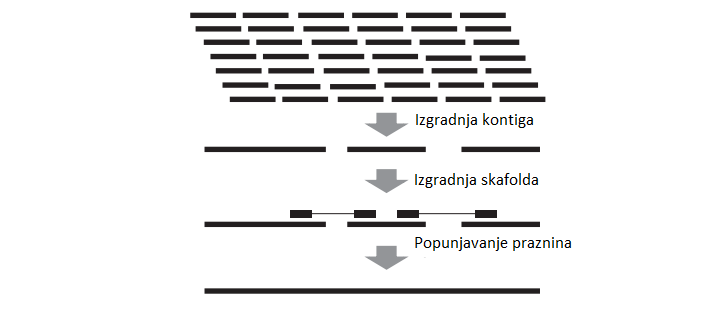
\includegraphics[width=0.9\textwidth]{cetvrta.PNG}
  \caption{Sekvencioniranje \textit{de novo} genoma za kratka očitavanja \cite{WingKinSung}}
  \label{fig:4}
\end{figure}

\section{Korekcija grešaka}
\label{poglavlje:korekcijaGresaka}

Ukoliko se neki k-mer pojavljuje u ulaznim očitavanjima jednom ili veoma mali broj puta, velika je verovatnoća da je on nastao kao posledica grešaka prilikom očitavanja i da ne treba da se nađe u rekonstruisanom genomu. Sa druge strane, za k-mer koji se pojavljuje veliki broj puta u ulaznim očitavanjima sa velikom sigurnošću se može tvrditi da nije posledica grešaka pri očitavanju. Ove razlike se mogu iskoristiti za filtriranje grešaka u k-merima i selektivno uklanjanje iz skupa podataka očitavanja koja sadrže greške \cite{WingKinSung}. 
Greške u očitavanjima mogu zbuniti \textit{de novo} asemblere. Da bi se to izbeglo, vrši se korigovanje tih grešaka pre početka asembliranja genoma.

\subsection{Brojanje k-mera}

Jedan konceptualno jednostavan, ali osnovni problem je \textbf{brojanje k-mera}. Brojanje k-mera se prvenstveno koristi u korekciji grešaka u očitavanjima, ali može biti korišćeno i u koraku asembliranja, detekciji ponovaka i kompresiji genomskih podataka. Ima značajnu ulogu u utvrđivanju da li je došlo do grešaka u očitavanju ili je u pitanju jednonukleotidni polimorfizam. 

Problem brojanja k-mera se definiše nad ulaznim skupom očitavanja i parametrom $k$. Iz ovog skupa, potrebno je izdvojiti podskup $Z$ svih mogućih k-mera i odrediti njihove frekvencije. Iako jednostavan problem, zbog velike količine podataka, on se ne može rešavati naivnim pristupima, već su potrebni napredni algoritmi i strukture podataka kako bi problem bio efikasno rešen. U nastavku će biti razmatrana četiri rešenja:
\begin{itemize}
\itemsep0em
    \item {Algoritam jednostavno heširanje}
    \item {Algoritam JellyFish}
    \item {Algoritam BFCounter}
    \item {Algoritam DSK}
\end{itemize}

\textbf{Jednostavno heširanje} - Problem brojanja k-mera može biti rešen implementacijom asocijativnog niza koristeći \textbf{heširanje}. Heširanje je tehnika kojom se vrši preslikavanje skupa ključeva na tabelu značajno manjih dimenzija. Idealno bi bilo da funkcija za svaki ključ
daje jedinstvenu poziciju. Ta funkcija naziva se \textbf{heš funkcija}, a tabela koja se koristi u tom
postupku zove se \textbf{heš tabela}. Kada je $k$ malo (npr. manje od 10), u procesu brojanja k-mera koristi se \textbf{savršeno heširanje}. Savršeno heširanje garantuje da neće doći do \textbf{kolizije}\footnote{Izraz koji potiče od latinske reči \textit{collisio} i znači sudar, sukob. U ovom kontekstu, moguće je da heš funkcija za dva različita k-mera da istu vrednost, te kažemo da su ta dva k-mera u koliziji, tj. sukobu.}. To je moguće kada se tačno zna koji skup ključeva će biti heširan prilikom dizajniranja heš funkcije. Ukoliko je $k$ veliko, algoritam jednostavnog heširanja će zahtevati previše prostora.

\textbf{Algoritam JellyFish} - Moguće je smanjiti prostornu složenost algoritma jednostavnog heširanja koristeći mehanizam \textbf{otvorenog adresiranja}. Otvoreno adresiranje je način rešavanja kolizije u heš tabelama. Kada se desi kolizija, traži se sledeća slobodna lokacija u heš tabeli za smeštanje vrednosti. Postoje tri metode otvorenog adresiranja: \textbf{linearno popunjavanje}, \textbf{kvadratno popunjavanje} i \textbf{duplo heširanje}. Mehanizam otvorenog adresiranja se koristi u algoritmu \textit{JellyFish} čija će implementacija detaljnije biti objašnjena u poglavlju \ref{odeljak:JellyFish}.

\textbf{Algoritam BFCounter} - U mnogim aplikacijama, od značaja su samo k-meri koji se pojavljuju najmanje $q$ puta. Kada bi moglo da se izbegne čuvanje k-mera koji se pojavljuju manje od $q$ puta, sačuvalo bi se mnogo memorije. Pol Melsted (engl. \textit{Páll Melsted}) je predložio algoritam  \textbf{BFCounter} koji broji samo k-mere koji se pojavljuju najmanje $q$ puta. On koristi \textit{counting Bloom} filter\footnote{Prostorno efikasna probabilistička struktura podataka koja dozvoljava dodavanje bilo kojih k-mera u nju i ispitivanje da li se k-mer pojavljuje najmanje $q$ puta.} da odredi da li se k-mer pojavljuje najmanje $q$ puta \cite{WingKinSung}.

\textbf{Algoritam DSK} - Iako je $BFCounter$ prostorno efikasan, njegova prostorna složenost i dalje zavisi od broja  k-mera u skupu očitavanja. Gijom Rizk (u originalu \textit{Guillaume Rizk}) predlaže algoritam koji se naziva \textbf{DSK}. Ideja ovog algoritma je da se skup k-mera podeli u različite liste tako da svaka lista bude smeštena na disk koristeći $D$ bitova. Zatim, za svaku listu, k-meri iz liste se dalje dele u podliste tako da svaka podlista može biti sačuvana u memoriji koristeći $M$ bitova. Na kraju, frekvencije k-mera u svakoj podlisti se izračunavaju algoritmom $JellyFish$. Algoritam $DSK$ će biti detaljno objašnjen u poglavlju \ref{odeljak:DSK}.

\begin{comment}

\newpage

\subsubsection{Jednostavno heširanje}

Problem brojanja k-mera može biti rešen implementacijom asocijativnog niza koristeći \textbf{heširanje}. Heširanje je tehnika kojom se vrsi preslikavanje skupa ključeva na tabelu značajno manjih dimenzija. Idealno bi bilo da funkcija za svaki ključ
daje jedinstvenu poziciju. Ta funkcija naziva se \textbf{heš funkcija}, a tabela koja se koristi u tom
postupku zove se \textbf{heš tabela}. Kada je $k$ malo (npr. manje od 10), u procesu brojanja k-mera koristi se \textbf{savršeno heširanje}. Savršeno heširanje garantuje da neće doći do \textbf{kolizije}\footnote{Izraz koji potiče od latinske reči \textit{collisio} i znači sudar, sukob. U ovom kontekstu, moguće je da heš funkcija za dva razlicita k-mera da istu vrednost, te kažemo da su ta dva k-mera u koliziji, tj. sukobu.}. To je moguće kada se tačno zna koji skup ključeva će biti heširan prilikom dizajniranja heš funkcije. Svaki k-mer $z$ može biti kodiran kao 2k-bitni binarni ceo broj \textit{b(z)} zamenom $A$, $C$, $G$ i $T$ u $z$ sa $00$, $01$, $10$, $11$, respektivno. Tako se izgrađuje tabela $Count[0..4^k - 1]$ veličine $4^k$ u kojoj svaka ulazna vrednost $Count[b(z)]$ čuva frekvenciju k-mera $z$ u skupu $Z$. Preciznije, prvo se vrši inicijalizacija svake ulazne vrednosti u $Count[0..4^k - 1]$ na 0. Zatim se iterativno skenira svaki k-mer $z$ iz $Z$ i uvećava $Count[b(z)]$ za 1. Na kraju, sve ulazne vrednosti različite od nule u $Count[]$ predstavljaju k-mere koji se pojavljuju u $Z$ kao i broj njihovih pojavljivanja.

\end{comment}

\begin{comment}
Slika \ref{fig:5}(a) predstavlja primer koji ilustruje ovaj jednostavni metod prebrojavanja.

\begin{figure}[!ht]
  \centering
  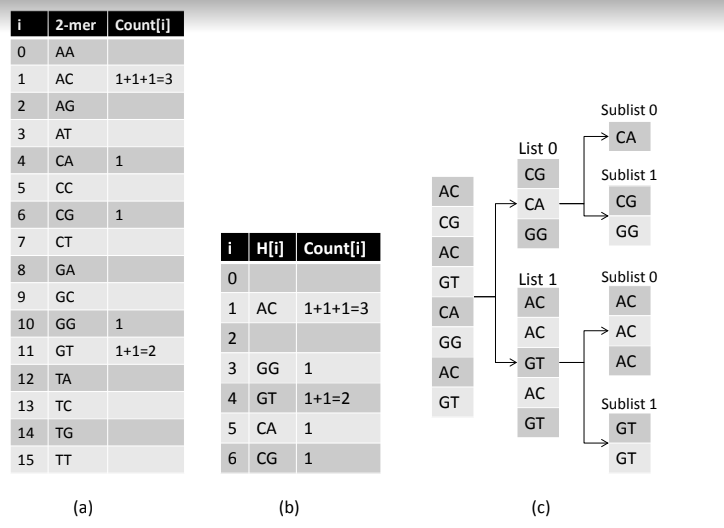
\includegraphics[width=\textwidth]{58_3algoritma.PNG}
  \caption{Razmatra se skup 4-mera $Z = \{AC; CG; AC; GT; CA; GG; AC; GT\}$: (a) Ilustruje jednostavan metod za brojanje k-mera koji koristi tabelu \textit{Count} veličine 4k. (b) Ilustruje \textit{JellyFish} metod brojanja k-mera koja koristi heš tabelu veličine 7. Heš funkcija je $h(z) = b(z)$ \textit{mod} $7$. Na primer, $GT$ se čuva u tabeli $Count$ sa indeksom 4, jer je $h(GT) = 4$. U ovom primeru se javlja je DNK kolizija. Pošto je i $h(CA) = 4$, $CA$ je u koliziji sa $GT$. Linearnim isprobavanjem $CA$ se ipak čuva u tabeli $Count$ sa indeksom 5. (c) Ilustruje DSK metod brojanja k-mera.
Pretpostavka je da je $h(z) = b(z)$, $n_{list} = 2$ i $n_{sublist} = 2$. DSK deli Z u
4 ($= n_{list} * n_{sublist}$) podliste, a zatim pokreće \textit{JellyFish} algoritam za brojanje k-mera u svakoj podlisti.}
  \label{fig:5}
  \source{\cite{WingKinSung}}
\end{figure}

Neka je $N = |Z|$. Tada je navedeni pristup veoma efikasan. Njegovo vreme izvršavanja je $O(N + 4^k)$, a kako treba izgraditi tabelu veličine $4^k$, prostorna složenost je $O(4^k)$. Kada je $k$ veliko, navedeni algoritam ne može da radi, jer zahteva previše prostora.

\end{comment}

\begin{comment}

\subsubsection{Algoritam JellyFish}
Moguće je smanjiti veličinu heš tabele koristeći mehanizam \textbf{otvorenog adresiranja}. Otvoreno adresiranje je način rešavanja kolizije u heš tabelama. Kada se desi kolizija, traži se sledeća slobodna lokacija u heš tabeli za smeštanje vrednosti. Postoje tri metode otvorenog adresiranja: \textbf{linearno popunjavanje}, \textbf{kvadratno popunjavanje} i \textbf{duplo heširanje}.

Ovaj mehanizam je iskorišćen u $JellyFish$ algoritmu. Uvodi se heš funkcija $h()$. Heš tabela $H[0..\frac{N}{\alpha} - 1]$ čuva niz k-mera iz $Z$, gde je $\alpha$ \textbf{faktor opterećenja}\footnote{Faktor opterećenja - broj koji kontroliše veličinu heš tabele.} $(0 < \alpha \leq 1)$. Svaki k-mer iz $Z$ je heširan u neku vrednost $H[i]$ gde je $i = h(z)$. Izgrađuje se tabela $Count[0..\frac{N}{\alpha} - 1]$, pri čemu $Count[i]$ čuva broj pojavljivanja za k-mer $H[i]$. Ukoliko pri heširanju funcijom $h()$ dođe do kolizije, ona se razrešava mehanizmom otvorenog adresiranja. Na ovaj način se pokušava smanjivanje prostora koji je potreban za obavljanje brojanja k-mera.


Neka je $h()$ heš funkcija i $H[0..\frac{N}{\alpha} - 1]$ heš tabela koja čuva niz k-mera, gde je $\alpha$ \textbf{faktor opterećenja}\footnote{Broj koji kontroliše veličinu heš tabele} $(0 < \alpha \leq 1)$. Potrebno je izgraditi tabelu $Count[0..\frac{N}{\alpha} - 1]$ gde $Count[i]$ čuva broj pojavljivanja za k-mer $H[i]$. Za svaki k-mer iz $Z$ vrši se njegovo  heširanje u neku vrednost $H[i]$ gde je $i = h(z)$. Ako $H[i]$ nije prazan i $H[i] \neq z$, ne možemo čuvati $z$ u $H[i]$, tj. došlo je do kolizije. Ona može biti razrešena pomoću mehanizma otvorenog adresiranja. Na primer, kolizija se može razrešiti \textbf{linearnim popunjavanjem}. Ovom metodom pokušavamo da uvećamo indeks $i$ za jedan kada se kolizija dogodi sve dok je $H[i] = z$ ili je ulaz $H[i]$ prazan. Nakon sto su svi k-meri iz $Z$ obrađeni i sve kolizije razrešene, prikazuje se $(H[i], Count[i])$ za sve ulaze $H[i]$ različite od nule.

Funkcija $hashEntry()$ sa slike \ref{fig:6} (donji deo slike) ilustruje šemu linearnog popunjavanja za razrešavanje kolizije. Ako $hashEntry(z, h, \frac{N}{\alpha})$ vraća prazan ulaz $H[i]$, onda $z$ ne postoji u heš tabeli i postavljamo $H[i] = z$ i $Count[i] = 1$. U suprotnom, ako $hashEntry(z, h, \frac{N}{\alpha})$ vraća ulaz $H[i] = z$, uvećavamo $Count[i]$ za jedan. Nakon sto su svi k-meri iz $Z$ obrađeni, prikazujemo $(H[i], Count[i])$ za sve ulaze $H[i]$ različite od nule.

Algoritam \textit{JellyFish} je detaljnije objašnjen na slici \ref{fig:6} (gorni deo slike), dok slika \ref{fig:5} (b) daje primer koji ga ilustruje. On je efikasniji, ukoliko ne postoji kolizija. U praksi je očekivani broj kolizija manji, ukoliko za faktor opterećenja važi $\alpha \leq 0.7$. Zatim, očekivano vreme izvršavanja je $O(N)$. Što se tiče prostorne složenosti, tabele $H[]$ i $Count[]$ zahtevaju $\frac{N}{\alpha}(2k + 32)$ bitova, pod pretpostavkom da broj zauzima 32 bita. Gore pomenuta ideja smanjivanja veličine heš tabele je iskorišćena u $JellyFish$ algoritmu.

\begin{figure}[!ht]
  \centering
  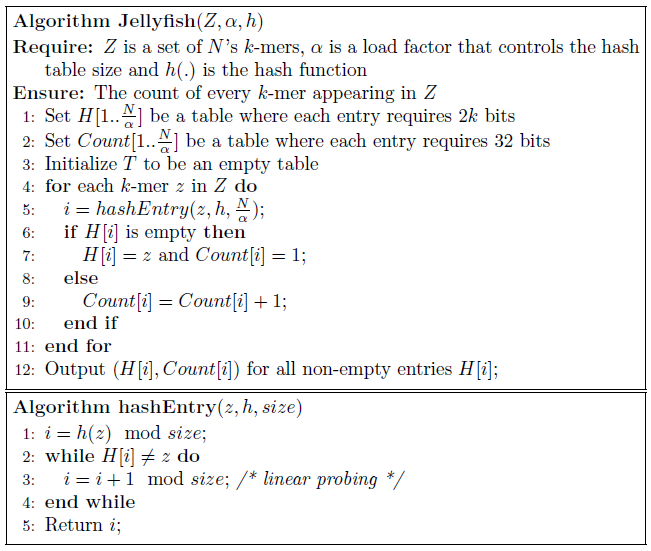
\includegraphics[width=0.85\textwidth]{Jellyfish5_9.PNG}
  \caption{Algoritam Jellyfish i funkcija hashEntry \cite{WingKinSung}}
  \label{fig:6}
\end{figure}

Iako algoritam $JellyFish$ koristi manje prostora od metode naivnog prebrojavanja, $JellyFish$ heš tabela mora biti veličine koja je jednaka bar broju jedinstvenih k-mera iz $Z$. $JellyFish$ i dalje zahteva mnogo memorije u slučaju da je broj jedinstvenih k-mera u $Z$ veliki.

\subsubsection{Algoritam \textit{BFCounter}}
U mnogim aplikacijama, od značaja su samo k-meri koji se pojavljuju najmanje $q$ puta. Kada bi moglo da se izbegne čuvanje k-mera koji se pojavljuju manje od $q$ puta, sačuvalo bi se mnogo memorije. Pol Melsted (engl. \textit{Páll Melsted}) je predložio algoritam  \textbf{BFCounter} koji broji samo k-mere koji se pojavljuju najmanje $q$ puta. On koristi \textit{counting Bloom} filter da odredi da li se k-mer pojavljuje najmanje $q$ puta. To je prostorno efikasna probabilistička struktura podataka koja dozvoljava dodavanje bilo kojih k-mera u nju i ispitivanje da li se k-mer pojavljuje najmanje $q$ puta. 

Iako on može dati pogrešno pozitivan rezultat (pogrešan izveštaj da k-mer postoji ili pogrešno proceniti broj k-mera), ne može dati pogrešno negativan rezultat. \textit{BFCounter} održava \textit{counting Bloom} filter $B$ i heš tabelu $H$ i sastoji od 2 faze. 

Prva faza počinje sa praznim \textit{counting Bloom} filterom $B$ i praznom heš tabelom $H$. U ovoj fazi se skeniraju k-meri iz $Z$ jedan po jedan. Za svaki k-mer $z\inZ$ se proverava da li se $z$ pojavljuje najmanje $q - 1$ puta u \textit{counting Bloom} filteru $B$ utvrđivanjem da li je $countBloom(x, B) \geq q-1$. Ako nije, vrši se umetanje $z$ u $Z$ pomoću $insertBloom(z, B)$. U suprotnom, $z$ se pojavljuje najmanje $q$ puta. Zatim se vrši proveravanje da li je $z$ u heš tabeli $H$. Ako nije, $z$ se umeće u neki prazan ulaz $H[i]$ i postavlja se $Count[i]$ na 0. 

U drugoj fazi se obavlja stvarno brojanje. Vrši se skeniranje k-mera iz $Z$ jedan po jedan. Za svaki k-mer $z$ iz $Z$, ako se $z$ pojavljuje u heširanom ulazu $H[i]$, onda se uvećava $Count[i]$ za 1.

Detaljan pseudokod je prikazan na slici \ref{fig:7}.

%Figura 5.10
\begin{figure}[h]
\centering
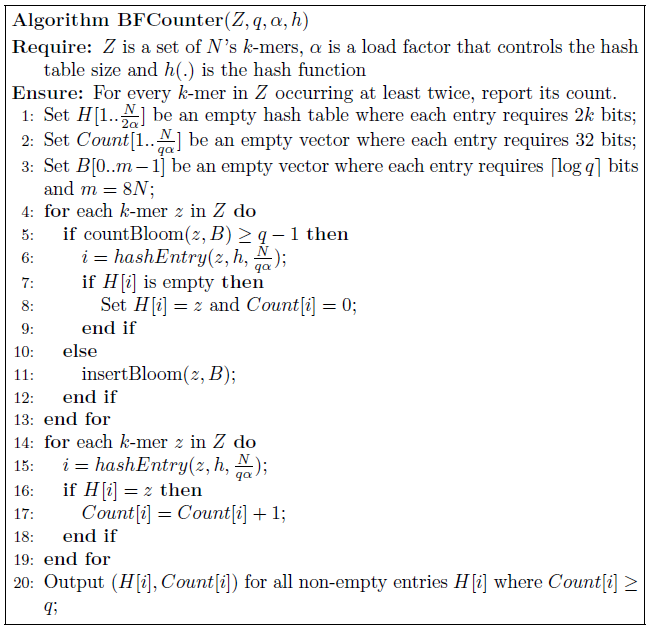
\includegraphics[width=12cm]{BFCounter5_10.PNG}
\caption{BFCounter \cite{WingKinSung}}
\label{fig:7}
\end{figure}


Vreme izvršavanja \textit{BFCounter} algoritma je $O(n)$. Što se tiče prostorne složenosti, \textit{counting Bloom} filter zahteva $O(N log(q))$ prostora. Prostor za $H[]$ i $Count[]$ je $\frac{N'}{\alpha}(2k + 32)$ bitova, gde je $N'$ broj k-mera koji se pojavljuju najmanje $q$ puta. Primetimo da je $N' \leq \frac{N}{q}$.

\end{comment}


\begin{comment}

\subsubsection{Algoritam DSK}
Iako je $BFCounter$ prostorno efikasan, njegova prostorna složenost i dalje zavisi od broja $N$ k-mera u $Z$. Neka je memorija fiksirana tako da bude $M$ bitova i neka je memorija diska fiksirana tako da bude $D$ bitova. Da li se može i dalje efikasno izračunati pojavljivanja k-mera? Gijom Rizk (engl. \textit{Guillaume Rizk}) nam daje pozitivan odgovor i predlaže metod koji se naziva \textbf{DSK}.

, a čiji pseudokod je prikazan na slici \ref{fig:63}.

%Figura 5.11
\begin{figure}[h]
\centering
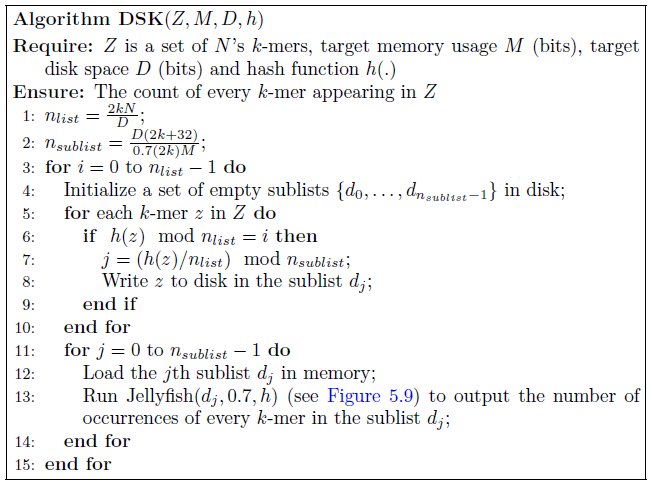
\includegraphics[width=12cm]{DSK5_11.PNG}
\caption{Algoritam DSK \cite{WingKinSung}}
\label{fig:63}
\end{figure}

Ideja ovog metoda je da se skup k-mera $Z$ podeli u različite liste tako da svaka lista bude smeštena na disk koristeći $D$ bitova. Zatim, za svaku listu, k-meri iz liste se dalje dele u podliste tako da svaka podlista može biti sačuvana u memoriji koristeći $M$ bitova. Na kraju, frekvencije k-mera u svakoj podlisti se izračunavaju algoritmom $JellyFish$.


\end{comment}

\begin{comment}
Preciznije, k-meri u $Z$ su podeljeni u $n_{list}$ lista približno slične dužine. Kako disk ima $D$ bitova i svaki k-mer može biti reprezentovan u 2k bitova, svaka lista može čuvati $l_{list} =  \frac{D}{2k}$ k-mera. Kako imamo $N$ k-mera u $Z$, postavlja se $n_{list} = \frac{N}{n_{list}} = \frac{2kN}{D}$. Ovo deljenje se obavlja heš funkcijom $h()$ koja ravnomerno mapira sve k-mere u $n_{list}$ lista. Preciznije, za svaki k-mer $z$ iz $Z$, $z$ se dodeljuje i-toj listi, ako je $h(z)$ \textit{mod} $n_{list} = i$. 

Zatim, svaka lista se dalje deli u podliste, pri čemu je svaka dužine $l_sublist$. Svaka podlista će biti obrađena u memoriji pomoću algoritma $JellyFish$, koji zahteva $\frac{l_{sublist}}{0.7}(2k +32)$ bitova. Kako memorija ima $M$ bitova, tako je $l_{sublist} = \frac{0.7M}{(2k + 32)}$.

Broj podlista je jednak $n_{sublist} = \frac{n_{list}}{n_{sublist}} = \frac{D(2k + 32)}{0.7(2k)M}$. Slično, svaka lista je podeljena u podliste heš funkcijom $h()$. Preciznije, za svaki k-mer $s$ u i-toj listi, $s$ je dodeljeno j-toj podlisti, ako je $(\frac{h(s)}{n_{list}})$ \textit{mod}
$n_{sublist} = j$.

Za svaku podlistu dužine $l_{sublist} = {0.7M}{2k + 32}$, koristeći $M$ bitova,  brojimo pojavljivanja svakog k-mera u podlisti koristeći $JellyFish(d_j, 0.7, h)$ sa slike \ref{fig:6}.

Na slici \ref{fig:5}(c) se može videti primer koji ilustruje izvršavanje algoritma DSK. Neka je $n_{list} = 2$, $n_{sublist} = 2$ and $h(z) = b(z)$ za svaki $z \in Z$. Kako je $n_{list} = 2$, algoritam izvršava 2 iteracije (u nastavku sledi opis nulte iteracije, jer se prva izvršava slično). Prva faza nulte iteracije skenira sve k-mere iz $Z$ i identifikuje svaki k-mer $z \in Z$ koji pripada nultoj listi. Na primer, $h(GG) = 10$, kako je $h(GG)$ \textit{mod} $n_{list} = 0$ i $\frac{h(z)}{n_{list}}$ \textit{mod} $n_{sublist} = 1$, $GG$ pripada nultoj listi i prvoj podlisti. Nakon toga, nulta lista se deli na nultu podlistu $\{CA\}$ i prvu podlistu $\{CG, GG\}$. Obe podliste su zapisane na disku. Druga faza čita svaku podlistu iz memorije i broji k-mere koristeći algoritam $JellyFish$.

Ovaj algoritam će zapisati samo jednom svaki k-mer iz $Z$, iako će svaki k-mer pročitati $n_{list}$ puta. Stoga, on neće generisati mnogo pristupa disku radi pisanja. Što se tiče vremenske složenosti, za i-tu iteraciju, algoritam numeriše sve k-mere u $Z$, što oduzima $O(n)$ vremena. Zatim, algoritam identifikuje $\frac{D}{2k}'s$ k-mera koji pripadaju i-toj listi i zapisuje ih na disk, što oduzima $O(\frac{D}{k})$ vremena. Nakon toga, algoritam  čita $\frac{D}{2k}'s$ k-mera i izvodi brojanje, što oduzima $O(\frac{D}{k})$ vremena. Tako da svaka iteracija zahteva $O(N + \frac{D}{k}) = O(N)$ vremena, gde je $N > \frac{D}{2k}$. Kako je $n_{list} = \frac{2kN}{D}$ broj iteracija, algoritam se izvršava u $O(kN^2)$ očekivanom vremenu. Kad je $D = \theta(N)$, algoritam se izvršava u $O(kN)$ očekivanom vremenu.

\end{comment}

\section{Konstrukcija kontiga}
\label{poglavlje:KonstrukcijaKontiga}

Nakon što su sva očitavanja korigovana, može se vršiti njihovo spajanje radi formiranja kontiga. Postoje dva pristupa za konstrukciju kontiga:
\begin{itemize}
\itemsep0em 
    \item{pristup baznog proširenja (\textit{base-by-base} pristup)}
    \item{De Brojnov grafovski pristup}
\end{itemize}

\subsection{Pristup baznog proširenja}

Pristup baznog proširenja rekonstruiše svaku kontigu tako što je proširuje bazu po bazu. Metod počinje tako što se nasumično bira očitavanje koje će služiti kao šablon. Zatim se očitavanja poravnavaju na oba kraja šablona ($5'$ kraj i $3'$ kraj). Na osnovu poravnanja se dobija \textbf{nukleotidna baza}\footnote{Baza koja se pojavljuje najveći broj puta na određenoj poziciji u poravnanju.} i šablon se njome proširuje.

Na slici \ref{fig:7} je prikazan jedan korak baznog proširenja.
Na vrhu je data sekvenca koja predstavlja šablon, a ispod nje sedam očitavanja poravnatih na $3'$ kraju šablona.

%Figure 5.12
\begin{figure}[!ht]
  \centering
  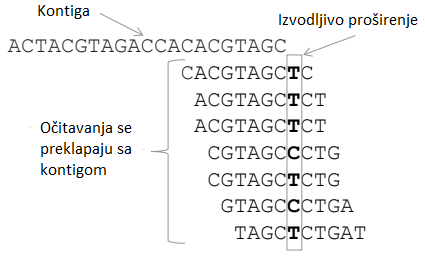
\includegraphics[width=0.7\textwidth]{contig5_12.PNG}
\caption{Jedan korak baznog proširenja \cite{WingKinSung}}
\label{fig:7}
\end{figure}

\noindent Pravougaonik pokazuje da su baze $C$ i $T$ izvodljivo proširenje šablona. Kako je $T$ konsenzusna baza, metod baznog proširenja će proširiti kontigu bazom $T$. Bazno proširenje se ponavlja sve dok ima konsenzusa. Zatim se prestaje sa proširenjem i dobija se kontiga. Proširenje se izvodi i na $3'$ kraju i na $5'$ kraju šablona.

\begin{comment}
Slika \ref{fig:8} daje pseudokod ovog metoda.

%Figure 5.13
\begin{figure}[!ht]
\centering
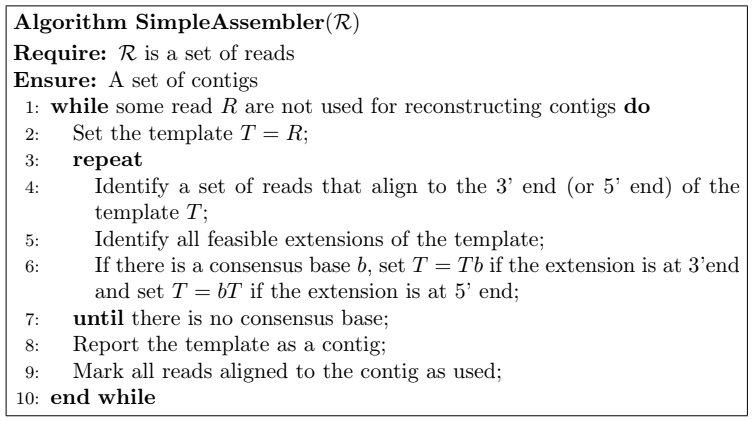
\includegraphics[width=0.9\textwidth]{SimpleAsembler5_13.PNG}
\caption{Jednostavan base-by-base asembler proširenja \cite{WingKinSung}} 
\label{fig:8}
\end{figure}

\end{comment}

Iako je bazno proširenje jednostavno, ono često daje kratke kontige zbog dva problema. Prvo, početni šablon je nasumično izabrano očitavanje. Ukoliko ono sadrži greške sekvencioniranja ili se nalazi u ponovku, to će uticati na proširenje. Drugi problem je što se može desiti da se šablon proširi u neki od ponovaka. Ponovak stvara grane koje gore navedeni pristup ne može da razreši.

\begin{comment}
Da bismo rešili prvi problem, biramo očitavanje za šablon, ako je malo verovatno da ono sadrži grešku sekvenciranja ili ako je malo verovatno da će biti u ponovljenom regionu. Koristeći ideju u sekciji 5.3.1, broje se frekvencije svih k-mera svih očitavanja. Očitavanje R se bira za šablon, ako su frekvencije svih njegovih k-mera unutar nekih korisnički definisanih pragova $\theta_{min}$ i $\theta_{max}$. Ako je broj pojavljivanja nekog k-mera manji od $\theta_{min}$, R će verovatno sadržati grešku sekvenciranja. Ako je broj pojavljivanja nekog k-mera veći od $\theta_{max}$, R će se verovatno naći u ponovljenom regionu. Ova dva praga mogu biti određena proučavanjem histograma frekvencija svih k-mera ulaznih sekvenci očitavanja.

Za drugi problem, rešenje je korišćenje informacija o povezivanju paired-end očitavanja za rešavanje nasumičnosti. Ovaj pristup je korišćen od strane $PE-asemblera [9]$. Figura 5.14 ilustruje tu ideju. Pretpostavimo da možemo proširiti šablon koristeći 2 različita očitavanja (crno i sivo). Ne možemo odlučiti koje je ispravo (pogledati Figuru 5.14(a)). Kako svako očitavanje ima svog para, možemo biti u stanju da donesemo odluku. Postoje 2 slučaja. U prvom slučaju, ako parnjak crnom očitavanju može biti poravnat sa šablonom, možemo verovati crnom očitavanju (Figura 5.14(b)). U drugom slučaju, pretpostavimo  da postoji nekoliko očitavanja R koja su poravnata sa šablonom i parnjaci od R mogu biti poravnati sa panjakom crnog očitavanja (pogledati Figuru 5.14(c)). Onda možemo verovati i crnom očitavanju. Drugim rečima, informacije o povezanosti paired-end očitavanja mogu pomoći u  filtriranju onih lažno pozitivnih poravnanja.
\end{comment}

\subsection{De Brojnov grafovski pristup}
\label{odeljak:DeBrojnovGraf}

\textbf{De Brojnov grafovski pristup} je zasnovan na De Brojnovim grafovima. Ovaj pristup su uveli Ramana Idjuri (engl. \textit{Ramana Idury}) i Majkl Voterman (engl. \textit{Michael Waterman}) u njihovoj knjizi \cite{Voterman}. Ovaj pristum je danas glavni za asembliranje kratkih očitavanja.

Neka je dat skup očitavanja $R$ i parametar $k$. De Brojnov graf je graf $H_k = (V, E)$, gde je $V$ skup svih k-mera skupa $R$, a $E$ skup svih grana u grafu. Ako su $u$ i $v$ prefiks dužine $k$ i sufiks dužine $k$ neke podniske dužine $k + 1$ iz $R$, respektivno, k-meri $u$ i $v$ formiraju granu $(u, v) \in E$. Pod pretpostavkom da je $N$ ukupna dužina svih očitavanja iz $R$, De Brojnov graf može biti konstruisan u $O(N)$ vremenu \cite{WingKinSung}. Algoritam za konstrukciju De Brojnovog grafa na osnovu očitavanja i parametra $k$ je implementiran u okviru ovog rada i biće detaljno opisan u poglavlju \ref{odeljak:ImplementacijaDB}.

Na slici \ref{fig:9}(a) je prikazan De Brojnov graf $H_2$ izgrađen na osnovu skupa k-mera $R = \{ACGC, CATC, GCA\}$, pri čemu je $\{AC, AT, CA, CG, GC, TC\}$ skup čvorova. Preklapanje k-mera koji odgovaraju granama grafa $H_2$ je prikazano na slici \ref{fig:9}(b).

%Figura 5.15
\begin{figure}[!ht]
\centering
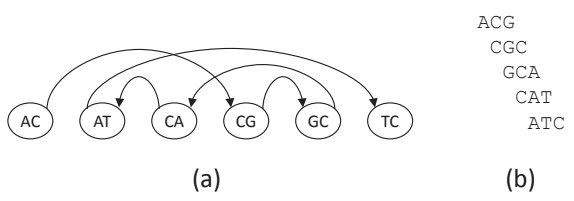
\includegraphics[width=0.7\textwidth]{Figura5_15.PNG}
\caption{Konstrukcija De Brojnovog grafa \cite{WingKinSung}}
 \label{fig:9}
 \end{figure}

Genomska sekvenca se može rekonstruisati identifikovanjem \textbf{Ojlerove putanje} grafa $H_k$. Ojlerova putanja je putanja koja obilazi svaku granu grafa $H_k$ tačno jednom. Ojlerova putanja grafa $H_k$ može biti izračunata u $O(n)$ vremenu, ako $H_k$ ima $n$ grana. Na primer, na slici \ref{fig:9}(a) postoji jedinstvena putanja od čvora $AC$ do čvora $TC$. Preklapanjem svih ivica 3-mera u redosledu putanje (slika \ref{fig:9}(b)) dobija se sekvenca $ACGCATC$. Sekvenca $ACGCATC$ je zapravo superstring formiran preklapanjem očitavanja i dobijen na osnovu De Brojnovog grafa za skup $R$. Međutim, Ojlerova putanja ne mora biti jedinstvena u $H_k$.

Neka je skup očitavanja $R = \{AAGATC, GATCGAT, CGATGA, ATGATT,\\ GATTT\}$ i neka je $k = 3$. U De Brojnovom grafu $H_3$ za dati skup $R$ postoje dva ciklusa, te će postojati i dve Ojlerove putanje. Na slici \ref{fig:10} je prikazan graf $H_3$.

%Figura 5.16
\begin{figure}[!ht]
\centering
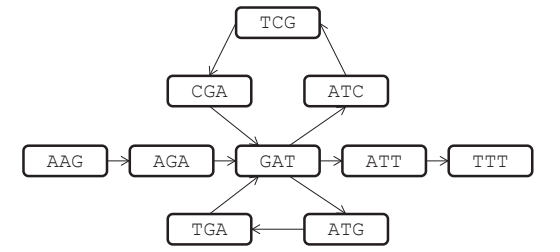
\includegraphics[width=0.7\textwidth]{Figura5_16.PNG}
\caption{De Brojnov graf sa dva ciklusa \cite{WingKinSung}}
\label{fig:10}
\end{figure}

\noindent Ukoliko se prvo obiđe gornji ciklus, dobija se $AAGATCGATGATTT$, a ukoliko se prvo obiđe donji ciklus, dobija se $AAGATGATCGATTT$. Primer sa slike \ref{fig:10} pokazuje da Ojlerova putanja možda neće uvek dati ispravnu sekvencu ili možda neće uvek postojati u nekom grafu $H_k$.

U nastavku će se govoriti o De Brojnovom grafovskom asembleru u slučaju kada:
\begin{itemize}
\itemsep0em 
    \item{ne postoji greška sekvencioniranja}
    \item{postoji greška sekvencioniranja}
\end{itemize}

\subsubsection{De Brojnov asembler bez greške sekvencioniranja}

Kako Ojlerova putanja nije jedinstvena i možda i ne postoji, ne teži se dobijanju kompletnog genoma. Umesto toga, teži se dobijanju skupa kontiga. U grafu $H_k$, kontiga predstavlja najdužu putanju čiji su svi čvorovi (osim početnog i krajnjeg) unutrašnjeg i spoljašnjeg stepena 1. Takva putanja se naziva maksimalnom prostom putanjom. 

\begin{comment}
Slika \ref{fig:11} daje pseudokod ovog jednostavnog metoda.


%Algoritam De Brojnov asembler
%Figura 5.17
\begin{figure}[!ht]
\centering
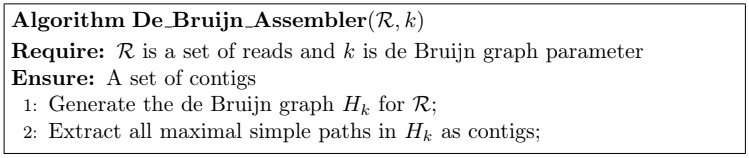
\includegraphics[width=0.9\textwidth]{Figura5_17.PNG}
\caption{Jednstavan De Brojnov grafovski asmbler \cite{WingKinSung}}
\label{fig:11}
\end{figure}

\end{comment}

Za De Brojnov graf $H_3$ sa slike \ref{fig:10} mogu se konstruisati četiri kontige: $AAGAT$, $GATCGAT$, $GATGAT$, $GATTT$. Parametar $k$ je veoma važan. Za različito $k$, mogu se dobiti različiti skupovi kontiga. Slika \ref{fig:12} ilustruje ovaj problem na De Brojnovom grafu za skup $R = \{AAGATC, GATCGAT, CGATGA, ATGATT,\\ GATTT\}$ u slučajevima kada je $k = 4$ i $k = 5$.

%Figura 5.18
\begin{figure}[!ht]
\centering
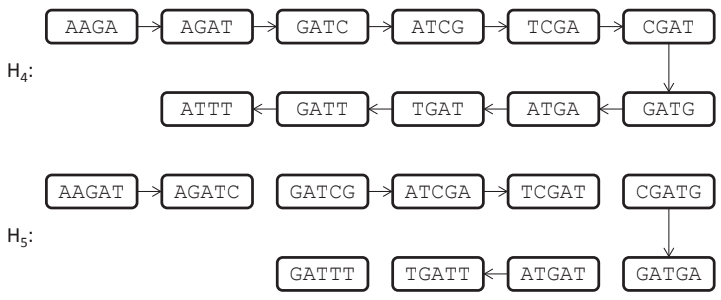
\includegraphics[width=0.9\textwidth]{Figura5_18.PNG}
\caption{De Brojnovi grafovi za $k = 4$ i $k = 5$ \cite{WingKinSung}}
\label{fig:12}
\end{figure}

Kada je $k = 4$, $H_4$ je prosta putanja i može se konstruisati jedna kontiga $AAGATCGATGATTT$. U slučaju da je $k = 5$, $H_5$ sadrži pet povezanih komponenti, svaka predstavlja prostu putanju i na osnovu toga može se konstruisati pet kontiga: $AAGATC$, $GATCGAT$, $CGATGA$, $ATGATT$, $GATTT$.

Prethodna razmatranja pokazuju da je izbor parametra $k$ veoma vazan. Kada je $k$ malo (pogledati $H_3$ na slici \ref{fig:10}), postoji veliki broj grana zbog ponovaka i rezultat je veliki broj kratkih kontiga. Kada je $k$ veliko (pogledati $H_5$ na slici \ref{fig:12}), neki k-meri nedostaju, što rezultuje nepovezanim komponentama, koje takođe generišu veliki broj kratkih kontiga. Zato je potrebno identifikovati adekvatno $k$ kako bi se pronašla ravnoteža između ova dva problema. Identifikacija adekvatnog $k$ biće opisana u nastavku teksta.

\subsubsection{De Brojnov asembler sa greškama sekvencioniranja}

Kod De Brojnovog asemblera bez grešaka sekvencioniranja pretpostavka je bila da ne postoje greške sekvencioniranja u očitavanjima, što je nerealno. Kada postoje greške, pokušava se njihovo uklanjanje redukovanjem šuma u De Brojnovom grafu. Rešenje koje će se razmatrati su predložili Danijel Zerbino (engl. \textit{Daniel Zerbino}) i Ivan Birni (enlg. \textit{Ewan Birney}). Kratka očitavanja imaju nisku stopu greške (sadrže jednu grešku na svakih 100 baza), a većina k-mera sadrži najviše jednu grešku. Ovakvi k-meri sa greškom mogu kreirati dve vrste anomalija u De Brojnovom grafu: \textbf{vrh (špic)} i \textbf{mehurić}.

\textbf{Vrh} je putanja dužine najviše $k$ gde svi unutrašnji čvorovi imaju ulazni i izlazni stepen 1, dok jedan od njihovih krajeva ima ulazni ili izlazni stepen 0. To može proizvesti potencijalnu kontigu dužine najviše $2k$.

Slika \ref{fig:13}(a) predstavlja višestruko poravnanje skupa od pet očitavanja, gde treće očitavanje ima grešku sekvencioniranja (prikazana podebljanim fontom). Slika \ref{fig:13}(b) predstavlja De Brojnov graf koji odgovara skupu očitavanja sa prvog dela slike i vrh koji je formiran usled jednog nepoklapanja u jednom očitavanju, tj. usled pomenute greške. Brojevi u zagradama označavaju mnogostrukost 4-mera (broj pojavljivanja 4-mera u očitavanjima). Ovaj vrh se može ukloniti iz De Brojnovog grafa, ali uklanjanje jednog vrha može generisati nove vrhove. Zbog toga, procedura uklanjanja mora uklanjati vrhove rekurzivno.

%Figure 5.19
\begin{figure}[!ht]
\centering
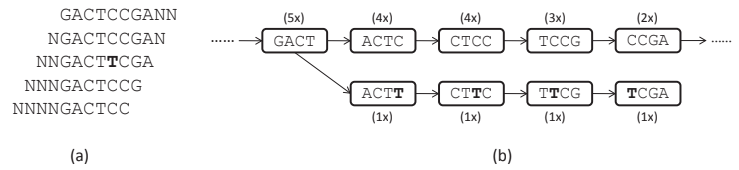
\includegraphics[width=\textwidth]{Figura5_19.PNG}
\caption{Formiranje vrha \cite{WingKinSung}}
\label{fig:13}
\end{figure}

% Ide pre ovaj vrh se može ukloniti Ako su svi čvorovi na vrhu %niske mnogostrukosti (k-meri koji se mali broj puta %pojavljuju u očitavanjima), takva kratka kontiga teško da %može biti ispravna (preformulisati).

\textbf{Mehurić} se sastoji od dve različite kratke putanje sa istim početnim i
krajnim čvorovima u De Brojnovom grafu, pri čemu su te dve putanje zapravo kontige koje se razlikuju u samo jednom nukleotidu. Na primer, slika \ref{fig:133}(a) sadrži skup očitavanja gde treće očitavanje ima jedno nepoklapanje. Slika \ref{fig:133}(b) prikazuje odgovarajući De Brojnov graf i jedan mehurić koji se formira.

%Figure 5.20
\begin{figure}[!ht]
\centering
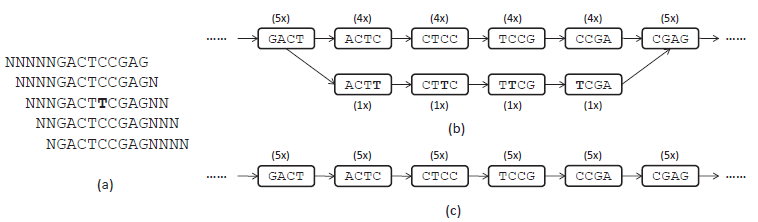
\includegraphics[width=\textwidth, height=5.3cm]{Figura5_20.PNG}
\caption{Formiranje mehurića \cite{WingKinSung}}
\label{fig:133}
\end{figure}

\noindent Gornja putanja mehurića predstavlja $GACTCCGAG$, dok donja putanja predstavlja $GACTTCGAG$. Kada su dve putanje u mehuriću veoma slične, putanja sa nižom mnogostukošću će verovatno biti ona koja će biti odbačena. Može se pokušati sa spajanjem mehurića. U ovom primeru, dve putanje imaju samo jedno nepoklapanje. Budući da su čvorovi u donjoj putanji niže mnogostrukosti, vrši se spajanje mehurića i dobija se graf na slici \ref{fig:13}(c). Preciznije, može se definisati \textbf{težina putanje} $w_1 \rightarrow w_2 \rightarrow ... \rightarrow w_p$ kao $\sum_{i=1}^{p} f(w_i)$, gde je $f(w_i)$ mnogostrukost od $w_i$. Prilikom spajanja dve putanje koje pripadaju istom mehuriću, zadržava se ona sa većom težinom.
\begin{comment}
Za spajanje mehurića, može se koristiti \textbf{algoritam turneje} (engl. \textit{tourbus algorithm}) koji će biti detaljno objašnjen u poglavlju \ref{odeljak:Tourbus}.
\end{comment}

\begin{comment}
Za spajanje mehurića, može se koristiti \textbf{algoritam turneje} (engl. \textit{tourbus algorithm}). Ovaj algoritam je nalik na Dijkstrinu pretragu u širinu baziranu na \textit{BFS} metodu. Algoritam počinje od proizvoljnog čvora $s$ i posećuje čvorove u rastućem poretku rastojanja od početnog čvora. Kada algoritam obrađuje neposećeni čvor $u$, on proverava i svako njegovo dete $v$. Za svako $v$ se izvode dva koraka. Prvo, dodeljuje se $u$ kao roditelj od $v$ u $BFS$ stablu postavljanjem $\pi (v) = u$. Drugo, ako je dete $v$ od $u$ posećeno, mehurić je detektovan. Algoritam izračunava najnižeg zajedničkog pretka $c$ od $u$ i $v$ u $BFS$ stablu definisanog sa $\pi ()$. Zatim se putanje $c \rightarrow u$ i $c \rightarrow v$ upoređuju. Ako su dovoljno slične, spajaju se. Zadržavamo putanju sa većom težinom.

Algoritam je detaljnije prikazan na slici \ref{fig:14}.



%Figure 5.21
\begin{figure}[!ht]
\centering
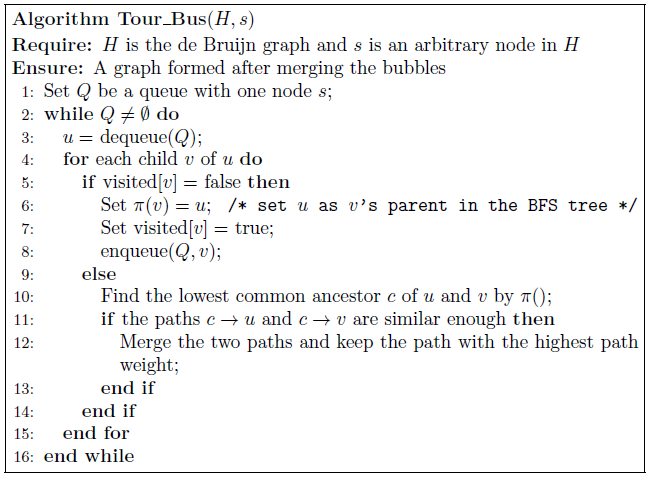
\includegraphics[width=0.8\textwidth]{Figura5_21.PNG}
\caption{Algoritam turneje \cite{WingKinSung}}
\label{fig:14}
\end{figure}


Slika \ref{fig:15} ilustruje korake algoritma turneje. Originalni De Brojnov graf je prikazan na slici \ref{fig:15}(a). Počevši od čvora $r$, \textit{BFS traversal} se izvodi kako bi se posetili svi potomci od $r$ u rastućem poretku rastojanja od $r$. \textit{BFS traversal} se zaustavlja kada dođe do posećivanja već posećenog čvora. Slika \ref{fig:15}(b) prikazuje BFS stablo (podebljano) kada je čvor $v$ ponovo posećen od strane čvora $u$. Identifikovanjem najnižeg zajedničkog pretka $c$ u BFS stablu, pronalaze se 2 putanje $c \rightarrow u$ i $c \rightarrow v$ koje formiraju mehurić. Vrši se spajanje 2 putanje i zadržava se putanja sa većom težinom. Nakon formiranja mehurića, dobija se slika \ref{fig:15}(c). Zatim se BFS nastavlja. Nakon što BFS poseti $u'$, ponovo posećuje $v'$. $c'$ je najniži zajednički predak od $u'$ i $v'$. Pronalaze se 2 putanje $c' \rightarrow u'$ i $c' \rightarrow v'$ koje formiraju mehurić. Nakon otklanjanja mehurića, dobija se slika \ref{fig:15}(d). Zatim, ne može se pronaći više nijedan mehurić i algoritam turneje se završava.



%Figure 5.22
\begin{figure}[!ht]
\centering
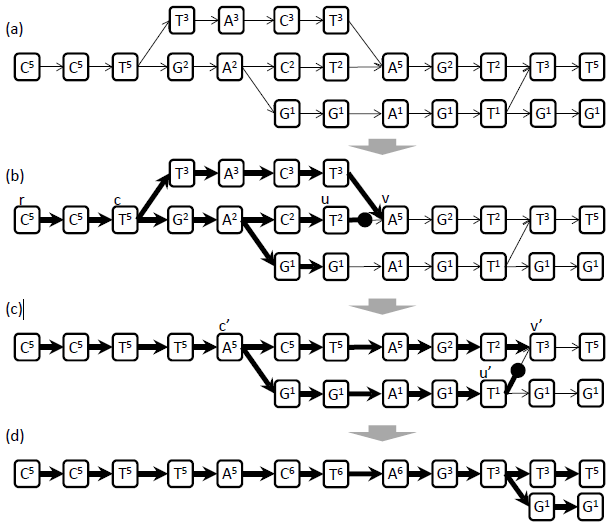
\includegraphics[width=0.8\textwidth]{Figura5_22.PNG}
\caption{Ovaj primer ilustruje kako algoritam turneje obilazi De Brojnov graf. Radi jasnoće, svaki čvor pokazuje poslednju bazu svojih k-mera i odgovarajući celobrojni stepen je njegova mnogostrukost. Algoritam izvodi pretragu u dobinu (BFS) i BFS stablo je prikazano podebljanim ivicama. Na slici (a) postoje 2 (ugnježdena) mehurića. Na slici (b) se izvodi BFS počevši od $r$. Kada se poseti $u$, dete $v$ od $u$ je posećeno. Identifikuje se mehurić i vrši se njegovo spajanje. Zatim, dobija se slika (c). Na slici (c) se nastavlja izvođenje BFS algoritma. Kada se posete $u'$, dete $v'$ od $u'$ je posećeno. Identifikuje se drugi mehurić i vrši se njegovo spajanje. Zatim se dobija slika (d). Na slici (d) se nastavlja izvođenje BFS algoritma. Kako se ne može identifikovati više nijedan mehurić, algoritam se završava.}
\label{fig:15}
\source{\cite{WingKinSung}}
\end{figure}

\end{comment}

Nakon što se uklone vrhovi i spoje mehurići u De Brojnovom grafu, može se dalje redukovati šum u grafu uklanjanjem k-mera sa mnogostrukošću manjom ili jednakom nekom pragu. 

Kombinovanjem ove tri tehnike: (1) otklanjanje vrhova, (2) spajanje mehurića i (3) filtriranje k-mera sa niskom mnogostrukošću dobija se algoritam \textit{Velvet} \cite{Velvet} za manipulaciju De Brojnovim grafovima i sastavljanje genomske sekvence.

\begin{comment}

i njegov psoudokod je prikazan na slici \ref{fig:16}.

%Figure 5.23
\begin{figure}[!ht]
\centering
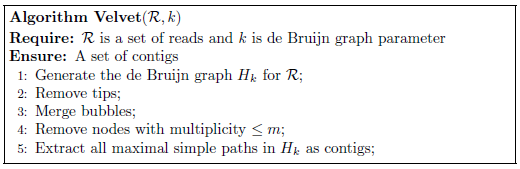
\includegraphics[width=0.9\textwidth]{Figura5_23.PNG}
\caption{Algoritam za otklanjanje grešaka sekvencioniranja \cite{WingKinSung}}
\label{fig:16}
\end{figure}

\end{comment}

\newpage

\subsection{Kako izabrati k?}
\label{poglavlje:IspravnoK}

Odabir parametra $k$ može značajno uticati na performanse De Brojnovog algoritma. Pokretanjem algoritma \textit{Velvet} za više različitih parametara $k$, može se izbeći odabir jedinstvenog $k$. Nakon izvršavanja ovog algoritma vrši se grupisanje i spajanje dobijenih kontiga. Jedan od problema je što kontige dobijene za različito $k$ imaju različit kvalitet. Kontige dobijene na osnovu $H_k$, gde je $k$ malo, veoma su tačne. Međutim, takve kontige su kratke, jer postoji veliki broj grana zbog ponovaka. Kontige dobijene na osnovu $H_k$ gde je $k$ veliko su duže, ali one mogu sadržati mnogo grešaka.

\textbf{IDBA asembler}\footnote{IDBA - \textit{A Practical Iterative de Bruijn Graph De Novo Assembler}.} počiva na ideji da ne treba graditi De Brojnov graf nezavisno za različite $k$. Umesto toga, \textit{IDBA} gradi De Brojnov graf $H_k$ postepeno krećući od malih $k$ i idući ka većim. Kada je $k$ malo, mogu se dobiti visokokvalitetne kontige, iako su kratke. Zatim se ove kontige koriste za ispravljanje grešaka u očitavanjima. Postepeno se izgrađuje De Brojnov graf $H_k$ za sve veće $k$. Kako su očitavanja u $R$ korigovana, to je šum u grafu $H_k$ redukovan. Na ovaj način se za veliko $k$ omogućava dobijanje dugih kontiga visokog kvaliteta. 

\begin{comment}

Na slici \ref{fig:17} se nalazi pseudokod koji opisuje ideju IDBA asemblera.

%Figure 5.24
\begin{figure}[!ht]
\centering
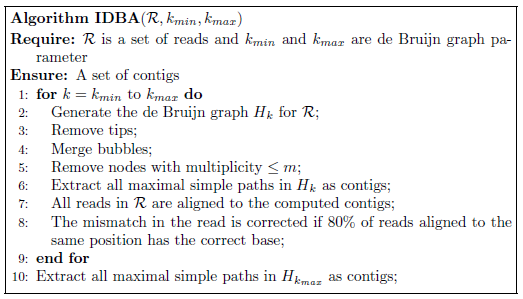
\includegraphics[width=0.9\textwidth]{Figura5_24.PNG}
\caption{IDBA \cite{WingKinSung}}
\label{fig:17}
\end{figure}

\end{comment}

\chapter{Implementirani algoritmi i rezultati}
\label{odeljak:algoritmiIRezultati}

U glavi \ref{poglavlje:Bio} data je biološka osnova i motivacija za algoritme koji se primenjuju u sekvencioniranju genoma. U ovom poglavlju će biti dati opisi implementacije tih algoritama u programskom jeziku Elixir sa osvrtom na njihovu prostornu i vremensku složenost, kao i opisi aplikacije i rezultati izvršavanja algoritama u okviru nje.

\section{Algoritam \textit{JellyFish}}
\label{odeljak:JellyFish}

Algoritam $JellyFish$ je algoritam koji se koristi za brojanje k-mera, a kao potprogram programa za korigovanje grešaka u očitavanjima. Pseudokod ovog algoritma dat je na slici \ref{box:jellyfish}.

\begin{comment}

\begin{figure}[!ht]
  \centering
  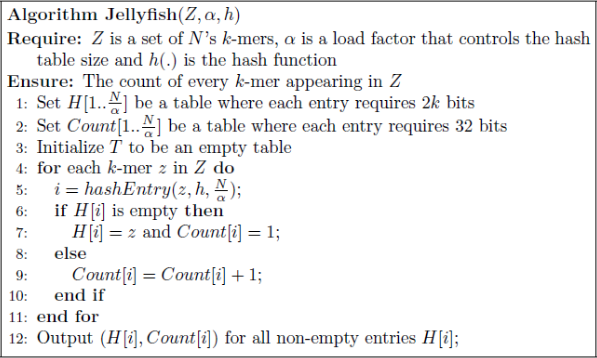
\includegraphics[width=0.9\textwidth]{Jellyfish.PNG}
  \caption{Algoritam Jellyfish \cite{WingKinSung}}
  \label{fig:jellyfish}
\end{figure}

\end{comment}

\begin{figure}[!ht]
\begin{tcolorbox}
\textbf{Algoritam JellyFish}(\textit{Z}, $\alpha$, \textit{h})

\textbf{Ulaz}: $Z$ je skup od $N$ k-mera, $\alpha$ je faktor opterećenja koji kontroliše veličinu heš tabele i $h$ je heš funkcija.

\textbf{Izlaz}: Broj pojavljivanja svakog k-mera u skupu \textit{Z}.

1: Kreirati praznu heš tabelu $H[1..\frac{N}{\alpha}]$ tako da svaki ulaz zahteva 2k bitova

2: Kreirati praznu tabelu $Count[1..\frac{N}{\alpha}]$ tako da svaki ulaz zahteva 32 bita 

3: foreach k-mer $z \in Z$ do:

4:\hspace{1cm} i = $hashEntry(z, h, \frac{N}{\alpha})$;
    
5:\hspace{1cm} if $H[i]$ is empty then

6:\hspace{2cm} $H[i] = z$ and $Count[i] = 1$;

7:\hspace{1cm} else 

8:\hspace{2cm} $Count[i] = Count[i] + 1$;

9:\hspace{1cm} end if

10: end for

11: Output $(H[i], Count[i])$ za sve ulaze $H[i]$ različite od 0.
\end{tcolorbox}
\caption{\textit{JellyFish} algoritam \cite{WingKinSung}}
\label{box:jellyfish}
\end{figure}

Neka je $h()$ heš funkcija i $H[0..\frac{N}{\alpha} - 1]$ heš tabela koja čuva niz k-mera, gde je $N = |Z|$ i $\alpha$ faktor opterećenja $(0 < \alpha \leq 1)$. Potrebno je izgraditi tabelu $Count[0..\frac{N}{\alpha} - 1]$, gde $Count[i]$ čuva broj pojavljivanja za k-mer $H[i]$. Za svaki k-mer iz $Z$ vrši se njegovo  heširanje u neku vrednost $H[i]$, gde je $i = h(z)$. Ako $H[i]$ nije prazan i $H[i] \neq z$, $z$ se ne može čuvati u $H[i]$, odnosno došlo je do kolizije. Ona može biti razrešena pomoću mehanizma otvorenog adresiranja. Na primer, kolizija se može razrešiti linearnim popunjavanjem. Kada se kolizija dogodi, indeks $i$ se uvećava za 1 sve dok se ne pronađe prvo prazno mesto $H[i]$ ili mesto gde je $H[i] = z$.

\begin{comment}

\begin{figure}[!ht]
  \centering
  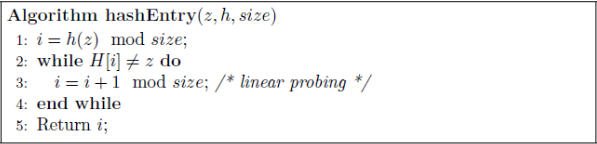
\includegraphics[width=0.9\textwidth]{HashEntry.PNG}
  \caption{Funkcija hashEntry \cite{WingKinSung}}
  \label{fig:hashEntry}
\end{figure}

\end{comment}

Funkcija $hashEntry()$ sa slike \ref{box:hashEntry} ilustruje šemu linearnog popunjavanja za razrešavanje kolizije. Ako $hashEntry(z, h, \frac{N}{\alpha})$ vraća prazan ulaz $H[i]$, onda $z$ ne postoji u heš tabeli i postavlja se $H[i] = z$ i $Count[i] = 1$. U suprotnom, ako $hashEntry(z, h, \frac{N}{\alpha})$ vraća ulaz $H[i] = z$, uvećava se $Count[i]$ za 1. Nakon sto su svi k-meri iz $Z$ obrađeni, prikazuje se $(H[i], Count[i])$ za sve ulaze $H[i]$ različite od 0.

\begin{figure}[!ht]
\begin{tcolorbox}
\textbf{Algoritam hashEntry}($H$, \textit{z}, $h$, \textit{size})

1: $i = h(z)$ mod \textit{size};

2: while $H[i] \neq z$ do

3:\hspace{1cm} $i = i + 1$ mod \textit{size}; $/$* linearno popunjavanje *$/$

4: end while

5: Return $i$;
\end{tcolorbox}
\caption{Funkcija \textit{hashEntry} \cite{WingKinSung}}
\label{box:hashEntry}
\end{figure}

\begin{comment}

\begin{figure}[!ht]
  \centering
  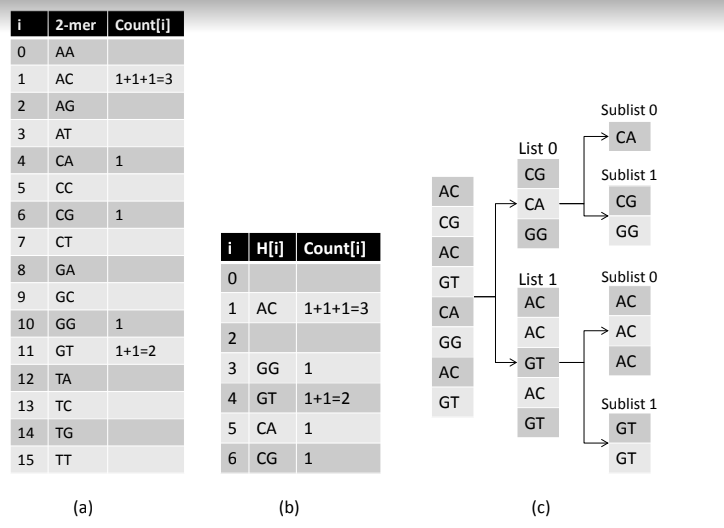
\includegraphics[width=\textwidth]{58_3algoritma.PNG}
  \caption{Razmatra se skup 4-mera $Z = \{AC; CG; AC; GT; CA; GG; AC; GT\}$: (a) Ilustruje jednostavan metod za brojanje k-mera koji koristi tabelu \textit{Count} veličine 4k. (b) Ilustruje \textit{JellyFish} metod brojanja k-mera koja koristi heš tabelu veličine 7. Heš funkcija je $h(z) = b(z)$ \textit{mod} $7$. Na primer, $GT$ se čuva u tabeli $Count$ sa indeksom 4, jer je $h(GT) = 4$. U ovom primeru se javlja jedna kolizija. Pošto je i $h(CA) = 4$, $CA$ je u koliziji sa $GT$. Linearnim isprobavanjem $CA$ se ipak čuva u tabeli $Count$ sa indeksom 5. (c) Ilustruje DSK metod brojanja k-mera.
Pretpostavka je da je $h(z) = b(z)$, $n_{list} = 2$ i $n_{sublist} = 2$. DSK deli Z u
4 ($= n_{list} * n_{sublist}$) podliste, a zatim pokreće \textit{JellyFish} algoritam za brojanje k-mera u svakoj podlisti.}
  \label{fig:5}
  \source{\cite{WingKinSung}}
\end{figure}

Slika \ref{fig:5}(b) daje primer koji ilustruje algoritam $JellyFish$. 
\end{comment}

Algoritam $JellyFish$ je efikasniji, ukoliko ne postoji kolizija. U praksi je očekivani broj kolizija manji, ukoliko za faktor opterećenja važi $\alpha \leq 0.7$. Zatim, očekivano vreme izvršavanja je $O(N)$. Što se tiče prostorne složenosti, tabele $H$ i $Count$ zahtevaju $\frac{N}{\alpha}(2k + 32)$ bitova, pod pretpostavkom da broj zauzima 32 bita \cite{WingKinSung}.

Skup očitavanja $Z$ je prilikom implementacije algoritma u programskom jeziku Elixir predstavljen listom, dok su za predstavljanje heš tabele $H$ i tabele \textit{Count} korišćene mape. Pri početnoj inicijalizaciji, vrednosti tabele $H$ se postavljaju na 0, a vrednosti tabele \textit{Count} na prazan string, dok im je skup ključeva isti. Početna inicijalizacija se vrši rekurzivno za svaki ključ. Izgled funkcija koje inicijalizuju tabele $H$ i $Count$, može se videti na listingu \ref{lst:103}. Argumenti pri pozivanju obe funkcije su prazna mapa ($\%\{\}$) i veličina mape koju treba kreirati. Pri svakom rekurzivnom pozivu, veličina mape se umanjuje za 1, a u mapu se dodaje novi element funkcijom \textit{Map.put/3} iz modula \textit{Map}. Kada veličina mape postane jednaka nuli, tada se izlazi iz rekurzije i funkcija vraća inicijalizovanu mapu. 

\lstinputlisting[language=erlang,label={lst:103},caption=Funkcije za inicijalizaciju $H$ i $Count$ tabele,captionpos=b]{103.ex}

\begin{comment}

JellyFish algoritam je detaljnije objašnjen na slici \ref{fig:6} (gorni deo slike), dok slika \ref{fig:5} (b) daje primer koji ga ilustruje. On je efikasniji, ukoliko ne postoji kolizija. U praksi je očekivani broj kolizija manji, ukoliko za faktor opterećenja važi $\alpha \leq 0.7$. Zatim, očekivano vreme izvršavanja je $O(N)$. Što se tiče prostorne složenosti, tabele $H[]$ i $Count[]$ zahtevaju $\frac{N}{\alpha}(2k + 32)$ bitova, pod pretpostavkom da broj zauzima 32 bita. Gore pomenuta ideja smanjivanja veličine heš tabele je iskorišćena u $JellyFish$ algoritmu.

\begin{figure}[!ht]
  \centering
  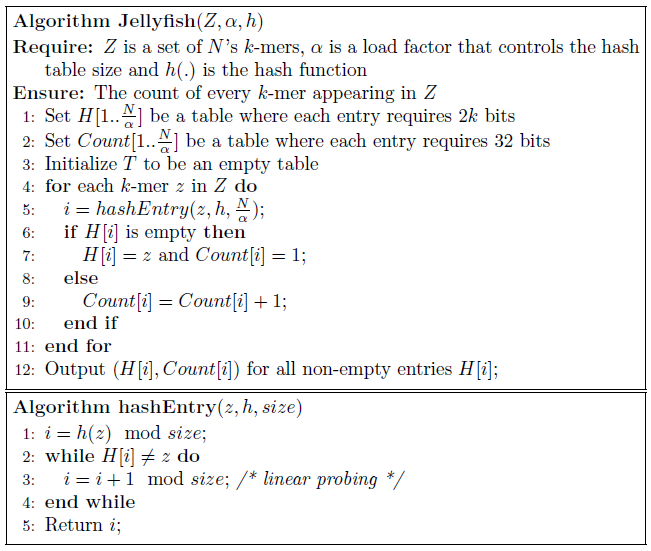
\includegraphics[width=0.85\textwidth]{Jellyfish5_9.PNG}
  \caption{Algoritam Jellyfish i funkcija hashEntry \cite{WingKinSung}}
  \label{fig:6}
\end{figure}

\end{comment}

\begin{comment}

Ulaz u glavnu funkciju:

\begin{itemize}
\itemsep0em 
    \item {$Z$ je skup od $N$ k-mera, koji je u Elixir-u predstavljen listom stringova}
    \item {$\alpha$ je faktor opterećenja koji kontroliše veličinu heš tabele i koji je broj tipa float između 0 i 1}
    \item {h je heš funkcija koja k-mere, tj. stringove mapira u brojeve}
\end{itemize}



Heš funkcija koja nosi naziv \textit{pattern\_to\_number} prikazana je na listingu \ref{lst:100}.

\lstinputlisting[language=erlang,label={lst:100},caption=Heš funkcija \textit{pattern\_to\_number},captionpos=b]{101.ex}

Argumenti funkcije su string koji predstavlja k-mer (\textit{pattern}), početni string koji je uvek prazan pri pozivu funkcije (\textit{begin\_string}), indeks  koji je uvek 0 pri pozivu funkcije (\textit{index}) i dužina k-mera (\textit{length\_of\_pattern}). Ova funkcija je rekurzivna i poziva se za svaki karakter stringa \textit{pattern}, počevši od nulte pozicije, sve dok se ne prođe kroz ceo string, tj. dok se \textit{index} ne izjednači sa \textit{length\_of\_pattern}. Dakle, uzima se prvi karakter \textit{pattern}-a, kodira se pomoćnom funkcijom \textit{symbol\_to\_number}, prikazanom na listingu \ref{lst:101} i nadovezuje se na \textit{begin\_string} pomoću operatora za nadovezivanje stringova $<>$. Zatim se prelazi na sledeći karakter, ponavlja se postupak i sve tako dok se ne dođe do kraja \textit{pattern}-a. U tom trenutku, povratna vrednost funkcije je \textit{begin\_string} koji umesto $A$, $C$, $G$ i $T$ sadrži kodove $00$, $01$, $10$, $11$, respektivno i koji se pomoću funkcije \textit{to\_integer/2} iz modula \textbf{String} pretvara u ceo broj.

\lstinputlisting[language=erlang,label={lst:101},caption=Pomoćna funkcija \textit{symbol\_to\_number},captionpos=b]{100.ex}

Glavna funkcija pre poziva pomoćnih funkcija obavlja početnu inicijalizaciju objekata koji su joj potrebni, tj. izračunava veličinu heš table $H$ i $Count$ tabele, a zatim ih inicijalizuje praznim stringovima i nulama, respektivno. Izgled glavne funkcije može se videti na listingu \ref{lst:102}.

\lstinputlisting[language=erlang,label={lst:102},caption=Glavna funkcija \textit{jellyfish\_algorithm},captionpos=b]{102.ex}

Funkcije za inicijalizaciju tabele H (\textit{build\_h\_table}) i Count tabele (\textit{build\_count\_table}), a koje su predstavljene mapama $h\_table$ i $count\_table$, identične su i imaju iste ulazne parametre. Jedina razlika je što su vrednosti mape $h\_table$ na početku prazni stringovi, a mape $count\_table$ nule, što se može videti na listingu \ref{lst:103}.

\lstinputlisting[language=erlang,label={lst:103},caption=Funkcije za inicijalizaciju H i Count tabela,captionpos=b]{103.ex}

Pomoćna funkcija koja obavlja brojanje k-mera je funkcija \textit{calculate} čiji su argumenti mape \textit{h\_table} i \textit{count\_table}, lista \textit{z\_table} i veličina pomenutih mapa \textit{size\_of\_H}. K$\hat{o}$d ove funkcije prikazan je na listingu \ref{lst:104}. 

\lstinputlisting[language=erlang,label={lst:104},caption=Pomoćna funkcija \textit{calculate},captionpos=b]{104.ex}

Kao što se može videti, funkcija \textit{calculate} je rekurzivna. Poziva se za svaki element liste \textit{z\_table}, počevši od njene glave, sve dok lista ne postane prazna. Za svaki string iz \textit{z\_table} prvo se poziva funkcija \textit{hashEntry} koja vrši heširanje stringova u indeks \textit{i} koji ključ za mape \textit{h\_table} i \textit{count\_table}. K$\hat{o}$d ove funkcije dat je listingom \ref{lst:105}.

\lstinputlisting[language=erlang,label={lst:105},caption=Pomoćna funkcija \textit{hashEntry},captionpos=b]{105.ex}

Zatim se proverava da li je vrednost ključa \textit{i} u mapi \textit{h\_table} prazan string. Vrednost ključa neke mape se u Elixir-u dohvata pomoću funkcije \textit{get/2} iz modula \textbf{Map} čiji su argumenti naziv mape i ključ. Ukoliko je vrednost prazan string, ključu se dodeljuje vrednost stringa koji se trenutno obrađuje i ključu u mapi \textit{count\_table} \textit{i} se dodeljuje vrednost 1. Vrednost ključa nekoj mapi se dodeljuje pomoću funkcije \textit{put/3} pomenutog modula. Njeni argumenti su naziv mape, ključ i vrednost koja se dodeljuje. Ako je vrednost ključa \textit{i} u mapi \textit{h\_table} različita od praznog stringa, onda se samo vrednost ključa \textit{i} u mapi \textit{count\_table}  povećava za jedan i prelazi se na obradu sledećeg stringa iz liste \textit{z\_table}. 

Na kraju, izlaz iz glavne funkcije je uređeni par $(\textit{h\_table}, \textit{count\_table})$. Kao što je već pomenuto, u Elixir-u su predstavljeni mapama veličine koja je količnik dužine liste \textit{z\_table} i faktora opterećenja \textit{alpha}. Obe mape imaju iste ključeve, dok su im vrednosti stringovi koji predstavljaju k-mere i brojevi koji predstavljaju broj pojavljivanja određenog stringa u listi \textit{z\_table}.

\end{comment}

\begin{comment}

Na listingu \ref{lst:106} se može videti konkretan primer izvršavanja algoritma u komandnom promptu.

\lstinputlisting[language=erlang,label={lst:106},caption=Primer pokretanja \textit{JellyFish} algoritma,captionpos=b]{jellyfish_pokretanje.ex}

Za kompajliranje fajla u kome se nalazi algoritam i pokretanje interaktivnog Elixir-a, navodi se komanda \textit{iex jellyfish.ex}. Nakon toga mogu se pozivati funkcije tako što se prvo navede ime modula u okviru koga su definisane, tačka, pa naziv funkcije i njeni argumenti. U ovom slučaju to su modul \textit{JellyFish}, funkcija \textit{jellyfish\_algorithm}, lista stringova $["AC", "CG", "AC", "GT", "CA","GG", "AC",\\"GT"]$ koji predstavljaju k-mere i faktor opterećenja 0.7.

\end{comment}

\section{Algoritam \textit{DSK}}
\label{odeljak:DSK}

Algoritam \textit{DSK} je još jedan algoritam za brojanje k-mera, ali vremenski i prostorno efikasniji od algoritma $JellyFish$. Na slici \ref{box:DSK} se može videti pseudokod ovog algoritma.

\begin{comment}

%Figura 5.11
\begin{figure}[h]
\centering
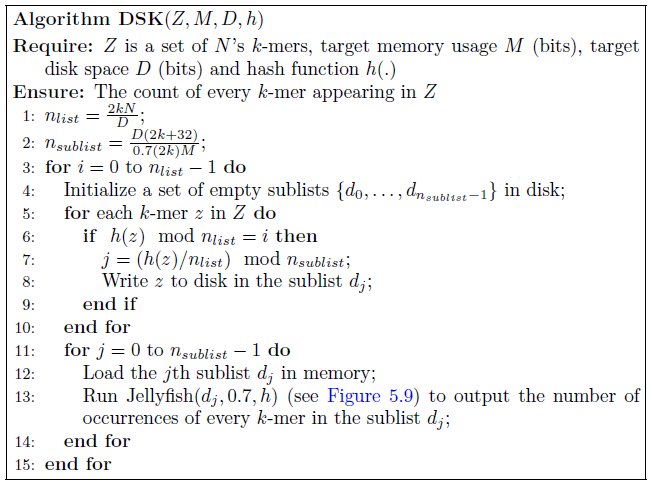
\includegraphics[width=0.9\textwidth]{DSK5_11.PNG}
\caption{DSK algoritam \cite{WingKinSung}}
\label{fig:DSK}
\end{figure}

\end{comment}

\begin{figure}[!ht]
\begin{tcolorbox}
\textbf{Algoritam DSK}(\textit{Z}, \textit{M}, \textit{D}, \textit{h})

\textbf{Ulaz}: $Z$ je skup od $N$ k-mera, $M$ (bitova) je veličina memorije za čuvanje lista, $D$ (bitova) je veličina diska za čuvanje podlista i \textit{h} je heš funkcija.

\textbf{Izlaz}: Broj pojavljivanja svakog k-mera u skupu \textit{Z}.

1: $n_{list} = \frac{2kN}{D}$;

2: $n_{sublist} = \frac{D(2k + 32)}{0.7(2k)M}$;

3: for $i = 0$ to $n_{list} - 1$ do

4:\hspace{1cm} Inicijalizovati skup praznih podlista ${d_0,..., d_{n_{sublist} - 1}}$ na disku

5:\hspace{1cm} for each k-mer $z \in Z$ do

4:\hspace{2cm} if $h(z)$ mod $n_{list} = i$ then

5:\hspace{3cm} $j = (h(z)$ div $n_{list})$ mod $n_{sublist}$;

6:\hspace{3cm} Upisati $z$ na disk u podlistu $d_j$

7:\hspace{2cm} end if

10:\hspace{1cm} end for

11:\hspace{1cm} for $j = 0$ to $n_{sublist} - 1$ do

12:\hspace{2cm} Učitaj j-tu podlistu $d_j$;

13:\hspace{2cm} Pokreni $JellyFish(d_j, 0.7, h)$ za ispisivanje broja pojavljivanja svakog k-mera u podlisti $d_j$

14:\hspace{1cm} end for

15: end for
\end{tcolorbox}
\caption{Funkcija \textit{DSK algoritam} \cite{WingKinSung}}
\label{box:DSK}
\end{figure}

Neka je dat skup k-mera $Z$, broj bitova $D$ na disku za čuvanje svake liste u koju se smeštaju k-meri, broj bitova $M$ u memoriji za čuvanje svake podliste k-mera i heš funkcija $h()$. Prvo se k-meri iz skupa $Z$ dele u $n_{list}$ lista približno slične dužine. Kako disk ima $D$ bitova i svaki k-mer može biti reprezentovan u $2k$ bitova, svaka lista može čuvati $l_{list} =  \frac{D}{2k}$ k-mera. Kako je $N$ broj k-mera u $Z$, to je $n_{list} = \frac{N}{n_{list}} = \frac{2kN}{D}$. Ovo deljenje se obavlja heš funkcijom $h()$ koja ravnomerno mapira sve k-mere u $n_{list}$ lista. Preciznije, za svaki k-mer $z$ iz skupa $Z$, $z$ se dodeljuje i-toj listi, ako je $h(z)$ \textit{mod} $n_{list} = i$. Zatim, svaka lista se dalje deli u podliste, pri čemu je svaka dužine $l_{sublist}$. Svaka podlista će biti obrađena u memoriji pomoću algoritma $JellyFish$, koji zahteva $\frac{l_{sublist}}{0.7}(2k +32)$ bitova. Kako memorija ima $M$ bitova, tako je $l_{sublist} = \frac{0.7M}{(2k + 32)}$. Broj podlista je  $n_{sublist} = \frac{n_{list}}{n_{sublist}} = \frac{D(2k + 32)}{0.7(2k)M}$. 

Svaka lista je podeljena u podliste heš funkcijom $h()$. Preciznije, za svaki k-mer $s$ u i-toj listi, $s$ je dodeljen j-toj podlisti, ako je $(\frac{h(s)}{n_{list}})$ \textit{mod} $n_{sublist} = j$. Za svaku podlistu dužine $l_{sublist} = {0.7M}{2k + 32}$, koristeći $M$ bitova,  vrši se brojanje pojavljivanja svakog k-mera u podlisti koristeći algoritam $JellyFish(d_j, 0.7, h)$ sa slike \ref{box:jellyfish}.

\textit{DSK} algoritam će zapisati samo jednom na disk svaki k-mer iz $Z$, iako će svaki k-mer pročitati $n_{list}$ puta. Stoga, algoritam neće generisati mnogo pristupa disku radi pisanja. Što se tiče vremenske složenosti, za i-tu iteraciju, algoritam numeriše sve k-mere u $Z$, što oduzima $O(N)$ vremena. Zatim, algoritam identifikuje $\frac{D}{2k}$ k-mera koji pripadaju i-toj listi i zapisuje ih na disk, što oduzima $O(\frac{D}{k})$ vremena. Nakon toga, algoritam  čita $\frac{D}{2k}$ k-mera i izvodi brojanje, što oduzima $O(\frac{D}{k})$ vremena. Tako da svaka iteracija zahteva $O(N + \frac{D}{k}) = O(N)$ vremena, gde je $N > \frac{D}{2k}$. Kako je $n_{list} = \frac{2kN}{D}$ broj iteracija, algoritam se izvršava u $O(kN^2)$ očekivanom vremenu. Kad je $D = \theta(N)$, algoritam se izvršava u $O(kN)$ očekivanom vremenu.

Heš funkcija $h()$, koja se koristi i u algoritmu $DSK$ i u algoritmu $JellyFish$, u okviru ovog rada je predstavljena funkcijom \textit{pattern\_to\_number} koja koristi pomoćnu funkciju \textit{symbol\_to\_number}. Pomoćna funkcija \textit{symbol\_to\_number} kodira nukleotide pomoću mape, gde su $A$, $T$, $C$ i $G$ ključevi sa vrednostima $00$, $01$, $10$, $11$, respektivno. Funkcija \textit{pattern\_to\_number} koristeći ovu funkciju rekurzivno kodira svako slovo niske \textit{pattern} koja predstavlja k-mer, počevši od nulte pozicije. Kodovi se nadovezuju na početnu praznu nisku $begin\_string$ pomoću operatora $<>$. Kada se obradi cela niska \textit{pattern}, izlazi se iz rekurzije i funkcija vraća nisku transformisanu u broj  koji predstavlja kodiran k-mer. Implementacija ovih funkcija u Elixir-u može se videti na listingu \ref{lst:106}.

\lstinputlisting[language=erlang,label={lst:106},caption=Funkcija \textit{pattern\_to\_number} i pomoćna funkcija \textit{symbol\_to\_number},captionpos=b]{106.ex}

\begin{comment}
Na slici \ref{fig:5}(c) se može videti primer koji ilustruje izvršavanje algoritma DSK. Neka je $n_{list} = 2$, $n_{sublist} = 2$ and $h(z) = b(z)$ za svaki $z \in Z$. Kako je $n_{list} = 2$, algoritam izvršava 2 iteracije (u nastavku sledi opis nulte iteracije, jer se prva izvršava slično). Prva faza nulte iteracije skenira sve k-mere iz $Z$ i identifikuje svaki k-mer $z \in Z$ koji pripada nultoj listi. Na primer, $h(GG) = 10$, kako je $h(GG)$ \textit{mod} $n_{list} = 0$ i $\frac{h(z)}{n_{list}}$ \textit{mod} $n_{sublist} = 1$, $GG$ pripada nultoj listi i prvoj podlisti. Nakon toga, nulta lista se deli na nultu podlistu $\{CA\}$ i prvu podlistu $\{CG, GG\}$. Obe podliste su zapisane na disku. Druga faza čita svaku podlistu iz memorije i broji k-mere koristeći $JellyFish$ algoritam.
\end{comment}

% Uzorak genoma se može predvideti identifikovanjem Ojlerove putanje. Međutim, Ojlerova putanja ne mora biti jedinstvena u De Brojnovom grafu ili čak ne mora ni postojati. Zbog toga se prelazi na De Brojnov grafovski pristup. (dopuni)

\section{Algoritam \textit{DeBrujinGraph}}
\label{odeljak:ImplementacijaDB}

De Brojnov grafovski pristup je jedan od pristupa u izgradnji kontiga koji se danas najčešće koristi. Cilj ovog algoritma je da pronađe sve kontige određene veličine, a uz pomoć De Brojnovog grafa. Slika \ref{box:DeBrujinAssembler} daje pseudokod ovog jednostavnog metoda koji na osnovu skupa očitavanja $R$ i parametra $k$ najpre izgrađuje De Brojnov graf $H_k$, a zatim pronalazi sve maksimalne proste putanje i od njih formira kontige.

\begin{comment}

%Algoritam De Brojnov asembler
%Figura 5.17
\begin{figure}[!ht]
\centering
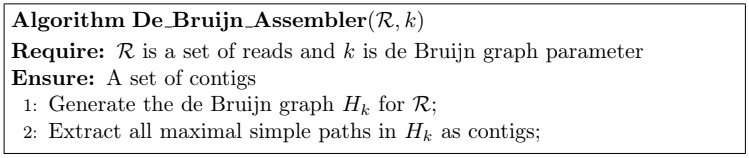
\includegraphics[width=0.9\textwidth]{Figura5_17.PNG}
\caption{Jednostavan De Brojnov grafovski asembler \cite{WingKinSung}}
\label{fig:11}
\end{figure}

\end{comment}

\begin{figure}[!ht]
\begin{tcolorbox}
\textbf{Algoritam $DeBrujinAssembler$}($R$, $k$)

\textbf{Ulaz}: $R$ je skup očitavanja i $k$ je parametar De Brojnovog grafa.

\textbf{Izlaz}: Skup kontiga $A$.

1: Generisati De Brojnov graf $H_k$ za skup $R$;

2: Izdvojiti sve maksimalne proste putanje u $H_k$ kao kontige;

\end{tcolorbox}
\caption{De Brojnov grafovski asembler \cite{WingKinSung}}
\label{box:DeBrujinAssembler}
\end{figure}

U okviru ovog rada, implementiran je algoritam \textit{DeBrujinGraph} koji se koristi u prvom koraku De Brojnovog grafovskog asemblera. Argumenti ovog alogoritma su string koji predstavlja jedno očitavanje iz skupa $R$ i parametar $k$. Prvi korak je kreiranje skupa k-mera na osnovu očitavanja i parametra $k$. Iz datog stringa koji predstavlja očitavanje izdvajaju se svi mogući podstringovi dužine $k$. Potom se formira skup jedinstvenih (k-1)-mera koji se pojavljuju kao prefiks ili sufiks nekog k-mera. Ovaj skup predstavlja skup čvorova budućeg De Brojnovog grafa. Zatim se za svaki k-mer vrši direktno povezivanje čvora koji predstavlja njegov prefiks sa čvorom koji predstavlja njegov sufiks. Na taj način se kreiran De Brojnov graf.

Povratna vrednost algoritma je mapa koja predstavlja De Brojnov graf. Svaki ključ mape predstavlja jedan čvor grafa, a njegova vrednost je lista stringova koji predstavljaju čvorove sa kojima pomenuti čvor formira granu. Primer pokretanja ovog algoritma biće dat u poglavlju \ref{odeljak:Rezultati}

\section{Algoritam \textit{AllEulerianCycles}}

U poglavlju \ref{odeljak:DeBrojnovGraf} je objašnjen pojam  Ojlerove putanje i značaj u procesu rekonstrukcije genoma. U tom procesu, algoritam za pronalaženje Ojlerove putanje je neophodan. Ovaj algoritam nije NP-kompletan i putanja se može efikasno pronaći \cite{skriptaBio}. Pseudokod pronalaženja Ojlerove putanje na osnovu De Brojnovog grafa može se videti na slici \ref{box:Ojler}. U okviru ovog rada implementiran je algoritam koji pronalazi sve Ojlerove putanje u grafu i njegov pseudokod se može videti na slici \ref{box:allEulerianCycles}. Rezultati njegovog pokretanja će detaljno biti prikazani u poglavlju \ref{odeljak:Rezultati}.
\vspace{0.2cm}

\begin{figure}[!ht]
\begin{tcolorbox}
\textbf{Problem Ojlerove putanje}: Pronaći Ojlerovu putanju u grafu.

Ulaz: Graf.

Izlaz: Putanja koja posećuje svaku granu u grafu tačno jednom.
\end{tcolorbox}
\caption{Problem Ojlerove putanje}
\label{box:Ojler}
\end{figure}

% U odeljku \ref{odeljak:ImplementacijaDB} je prikazano kako se na osnovu očitavanja i parametra $k$ može konstruisati De Brojnov graf. Konstruisani graf se može iskoristiti kao primer grafa u kome se pronalaze sve Ojlerove putanje. 

Pri pronalaženju svih Ojlerovih putanja u grafu problem je što neki čvorovi mogu imati više izlaznih i ulaznih grana, te se ne može jednoznačno odrediti čvor koji treba sledeći da se poseti. Broj ulaznih grana u dati čvor naziva se \textbf{ulazni stepen} čvora, a broj izlaznih grana iz datog čvora \textbf{izlazni stepen} čvora. Sa druge strane, u prostom usmerenom grafu u kome svaki čvor ima i ulazni i izlazni stepen jednak 1, može se jednoznačno odrediti naredni čvor koji treba da se poseti, jer u takvom grafu postoji samo jedan Ojlerov ciklus. Ideja algoritma \textit{AllEulerianCycles} je da se usmereni graf koji sadrži $n \geq 1$ Ojlerovih ciklusa transformiše na $n$ prostih usmerenih grafova koji sadrže tačno jedan Ojlerov ciklus. Ova transformacija ima svojstvo da je lako invertibilna, odnosno na osnovu jedinstvenog Ojlerovog ciklusa jednog od prostih usmerenih grafova moguće je rekonstruisati originalni Ojlerov ciklus polaznog grafa.

Neka je dat čvor $v$ iz grafa $G$ koji ima ulazni stepen veći od 1 sa ulaznom granom $(u, v)$ i izlaznom granom $(v, w)$. Konstruiše se jednostavniji $(u, v, w)$-obilazni graf u kome se uklanjaju grane $(u, v)$ i $(v, w)$, a dodaje se novi čvor $x$ zajedno sa granama $(u, x)$ i $(v, x)$. Nove grane $(u, x)$ i $(v, x)$ u obilaznom grafu nasleđuju oznake uklonjenih grana $(u, v)$ i $(v, w)$, respektivno. S obzirom na ulaznu granu $(u, v)$ u čvor $v$, koji ima $k$ izlaznih grana $(v, w_1)$,..., $(v, w_k)$, može se konstruisati $k$ različitih obilaznih grafova. Nikoja dva obilazna grafa nemaju isti Ojlerov ciklus. Cilj je iterativno konstruisati svaki mogući obilazni graf za dati graf sve dok se ne dobije velika porodica prostih usmerenih grafova. Svaki od ovih grafova će odgovarati različitom Ojlerovom ciklusu datog grafa \cite{bioinformaticsAlg}.

\begin{figure}[!ht]
\begin{tcolorbox}
\textbf{Algoritam AllEulerianCycles}(\textit{graph})

\textbf{Ulaz}:  De Brojnov graf \textit{graph}.

\textbf{Izlaz}: Sve Ojlerove putanje u De Brojnovom grafu \textit{graph}.

1: \textit{AllGraphs} $=$ skup koji se sastoji samo od jednog grafa \textit{graph}

2: while postoji složeni graf $G$ u skupu $AllGraphs$

3:\hspace{1cm} v $=$ čvor sa ulaznim stepenom većim od 1 u grafu G

4:\hspace{1cm} foreach ulazna grana $(u, v)$ u čvor $v$
    
5:\hspace{2cm} \textit{NewGraph} $=$ $(u, v, w)$-obilazni graf grafa $G$

6:\hspace{2cm} if \textit{NewGraph} je povezan

7:\hspace{3cm} Dodati \textit{NewGraph} u skup \textit{AllGraphs}

8:\hspace{1cm} Ukloniti graf $G$ iz skupa \textit{AllGraphs}

9: foreach graf $G$ iz skupa \textit{AllGraphs}

10:\hspace{1cm} Output Ojlerov ciklus u $G$
\end{tcolorbox}
\caption{Algoritam \textit{AllEulerianCycles} \cite{bioinformaticsAlg}}
\label{box:allEulerianCycles}
\end{figure}

Implementacija algoritma \textit{AllEulerianCycles} se sastoji od velikog broj funkcija. Na taj način je posao koji obavlja ovaj algoritam podeljen na smislene celine. Na primer, funkcija \textit{degree(g\_graph, v\_node)} izračunava ulazni i izlazni stepen za zadati čvor \textit{v\_node} i graf \textit{g\_graph}. Graf je predstavljen mapom. Ključ mape je čvor grafa, a lista vrednosti ključa čvorovi sa kojima ključ gradi grane u grafu. Funkcija \textit{degree} koristi pomoćnu funkciju \textit{iterate\_values/3} koja  prima tri argumenta: listu čvorova koju čine svi ključevi grafa, čitav graf i trenutni čvor. Implementacija ovih funkcija u Elixir-u može se videti na listingu \ref{lst:107}.

Izračuvanavanje izlaznog stepena \textit{out\_degree} za zadati čvor vrši se izračunavanjem dužine liste vrednosti u mapi za zadati čvor. Dohvatanje liste vrednosti za zadati čvor mape obavlja se funkcijom \textit{Map.get/2} iz modula \textit{Map}, a izračunavanje dužine liste funkcijom \textit{Kernel.length/1}.

Izračunavanje ulaznog stepena za zadati čvor vrši se pomoćnom funkcijom \textit{iterate\_values}. Ona rekurzivno za svaki ključ, odnosno čvor mape, proverava da li se zadati čvor nalazi u listi vrednosti tog čvora mape. Ako se nalazi, ulazni stepen \textit{in\_degree} zadatog čvora se uvećava za jedan i prelazi se na obradu sledećeg čvora mape. U suprotnom, prelazi se na sledeći čvor mape bez uvećavanja ulaznog stepena. Provera da li se zadati čvor nalazi u listi vrednosti trenutnog čvora vrši se funkcijom \textit{Enum.member?/2} iz modula \textit{Enum}. Kada se obradi i poslednji čvor mape, izlazi se iz rekurzije i vraća izračunati ulazni stepen čvora. Povratna vrednost funkcije \textit{degree} je uređeni par $(\textit{in\_degree}, \textit{out\_degree})$.

\lstinputlisting[language=erlang,label={lst:107},caption=Funkcija \textit{degree(g\_graph, v\_node)},captionpos=b]{107.ex}

\section{Uputstvo za pokretanje aplikacije}

Celokupna implementacija grafičkog korisničkog interfejsa i algoritama je dostupna i može se preuzeti sa adrese \cite{GIT}.
Kako Elixir nema naprednu podršku za grafički korisnički interfejs i to nije njegova osnovna namena, za potrebe ovog rada iskorišćena je i podrška programskog jezika Python i integrisanog razvojnog okruženja \textbf{\textit{PyCharm}} \cite{PyCharm}.

% Nakon preuzimanja implementacije i izvršenih koraka iz poglavlja \ref{odeljak:Instalacija}, potrebno je preuzeti i instalaciju za neko od integrisanih razvojnih okruženja za programski jezik Python. Za potrebe ovog rada izabran je \textit{\textbf{PyCharm}} i instalacija se može preuzeti sa njegove zvanične stranice \cite{PyCharm}. 

Projekat je organizovan tako da se sastoji od četiri foldera: \textit{data\_files}, \textit{result\_files}, \textit{source\_files} i \textit{executables}. U folderu \textit{data\_files} nalaze se tekstualni fajlovi koji sadrže ulazne podatke na kojima je moguće testirati implementirane algoritme (\textit{JellyFishData.txt}, \textit{DSKData.txt}, \textit{DeBrujinGraphData.txt}, \textit{AllEulerianCyclesData.txt}). U folderu \textit{result\_files} nalaze se tekstualni fajlovi u kojima se nalaze rezultati izvršavanja algoritama (\textit{JellyFish.txt}, \textit{DSK.txt}, \textit{DeBrujinGraph.txt}, \textit{AllEulerianCycles.txt}). Format ulaznih i izlaznih fajlova za svaki pojedinačni algoritam biće opisan u poglavlju \ref{odeljak:Rezultati}. Folder \textit{source\_files} sadrži izvorne fajlove u programskom jeziku Elixir u kojima se nalazi implementacija algoritama (\textit{jellyfish.exs}, \textit{dsk.exs}, \textit{debrujin\_graph.exs}, \textit{all\_eulerian\_cycles.exs}). Izvršne verzije izvornih fajlova nalaze se u folderu \textit{executables}. Pored ova četiri foldera, projekat sadrži i \textit{.py} fajl (\textit{interface.py}) u kome se nalazi interfejs koji sjedinjuje algoritme u jedinstvenu aplikaciju.

%Preduslovi da bi se projekat koristio/prevodio potrebno je da...

Implementirani algoritmi se mogu pokretati direktno uz pomoć Elixir interpretera. Potrebno je izvršiti komandu \textit{elixir ime\_algoritma.exs} ili \textit{iex ime\_algoritma.exs} za kojom slede argumenti u zagradi. Izvršne verzije Elixir fajlova se mogu pokretati iz komandne linije i bez instaliranja Elixir-a. Python interfejs podrazumeva korišćenje izvršnih programa. Za dobijanje izvršnih programa iz \textit{.exs} fajlova potrebno je izvršiti sledeće korake u komandnoj liniji:

\begin{itemize}
\itemsep0em 
    \item {pozicionirati se na lokaciju gde zelite da kreirate projekat}
     \item {izvršiti komandu \textit{mix new ime\_projekta}}
     \item {kompajlirati projekat pomoću komande \textit{mix} ili \textit{mix compile} u roditeljskom direktorijumu}
     \item {u \textit{lib} folderu projekta kreirati novi folder koji nosi naziv željenog algoritma i u njemu fajl \textit{cli.ex} koji ima sadržaj kao na listingu \ref{lst:cli}
     \item {u \textit{lib} folder prekopirati izvorni fajl algoritma}
     \item {izvršiti komandu \textit{mix escript.build} u roditeljskom direktorijumu}
\end{itemize}

\noindent Nakon izvršenih komandi, u roditeljskom direktorijumu će se pojaviti izvršna verzija izvornog fajla.

\lstinputlisting[language=erlang,label={lst:cli},caption=Sadržaj fajla \textit{cli.ex},captionpos=b]{cli.ex}


\section{Opis aplikacije i primeri upotrebe}

Svi algoritmi su implementirani u programskom jeziku Elixir. Elixir omogućava brzu obradu velike količine podataka veoma je tolerantan na greške, te ga to čini dobrim izborom za probleme bioinformatičke prirode. U nastavku će biti dat kratak prikaz i opis funkcionalnosti koje pruža implementirani interfejs, a potom i primeri pokretanja algoritama za izabrane ulazne fajlove.

\subsection{Opis aplikacije}

Pri pokretanju aplikacije otvara se glavni prozor koji se može videti na slici \ref{fig:glavniProzor}. Klikom na padajuću listu mogu se videti dostupni algortmi za izvršavanje, a potom i izabrati neki od njih. Prikaz padajuće liste i izbor jednog od algoritama može se videti na slici \ref{fig:padajucaLista}. 

\begin{figure}[h]
\centering
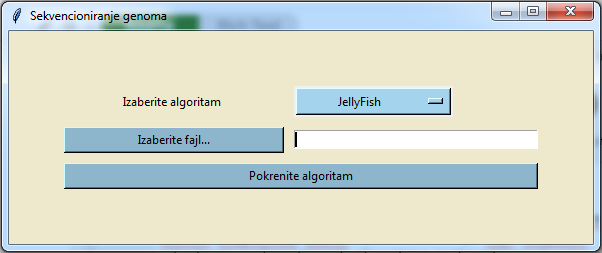
\includegraphics[width=\textwidth]{glavni_prozor.PNG}
\caption{Glavni prozor programa}
\label{fig:glavniProzor}
\end{figure}

\begin{figure}[h]
\centering
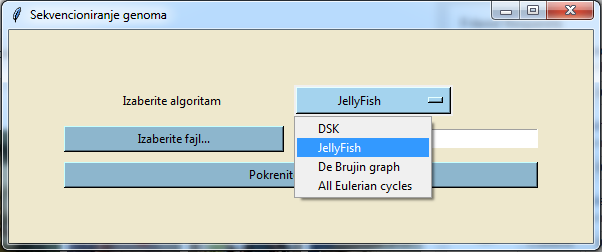
\includegraphics[width=\textwidth]{padajuca_lista.PNG}
\caption{Izbor algoritma}
\label{fig:padajucaLista}
\end{figure}

Nakon toga je potrebno izabrati fajl iz kojeg će se čitati ulazni podaci. Klikom na dugme \textit{Izaberite fajl...} otvara se novi dijalog u okviru kojeg se može izabrati ulazni tekstualni fajl, što se može videti na slici \ref{fig:fileChooser}.

\begin{figure}[h]
\centering
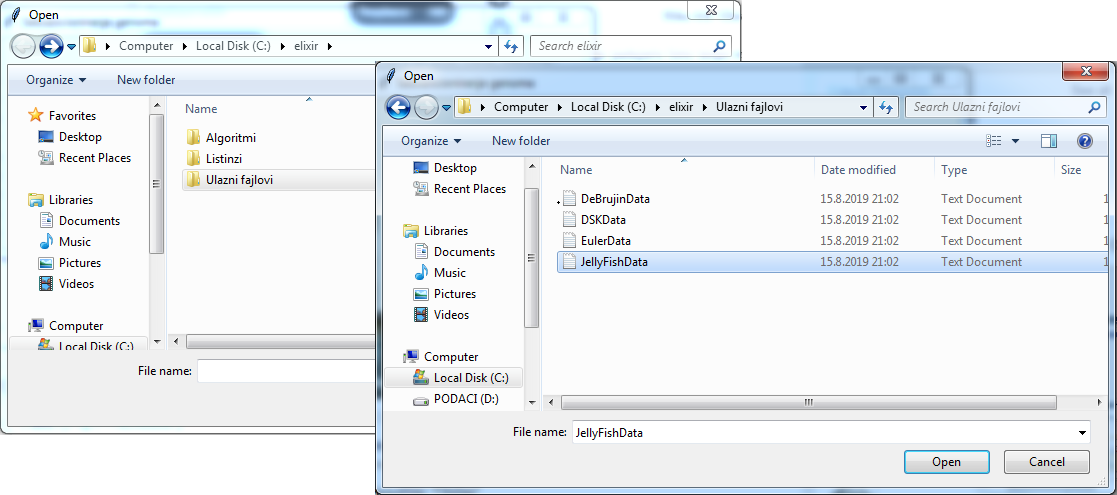
\includegraphics[width=\textwidth]{file_chooser3.PNG}
\caption{Izbor ulaznog fajla}
\label{fig:fileChooser}
\end{figure}

Na kraju je potrebno pokrenuti algoritam klikom na dugme \textit{Pokrenite algoritam}. U pozadini se pokreće odgovarajići izvršni fajl algoritma sa argumentima koji su pročitani iz ulaznog fajla. Na ovaj način se izbegava kompajliranje fajla u kome se nalazi implementacija algoritma pri svakom kliku na dugme za pokretanje. Pritom se omogućava i izvršavanje algoritama na mašini na kojoj ne postoji instaliran Elixir.

Ukoliko je algoritam uspešno izvršen, rezultati pokretanja će biti upisani u odgovarajući tekstualni fajl i pojaviće se obaveštenje o uspešnom izvršavanju i nazivu rezultujućeg fajla. Prikaz ovog obaveštenja dat je na slici \ref{fig:uspesnoIzvrsavanje}.

% Nakon toga je potrebno izabrati fajl iz kojeg će se čitati ulazni podaci. Klikom na dugme \textit{Izaberite fajl...}, otvara se prozor u okviru kojeg se može izabrati ulazni tekstualni fajl, što se može videti na slici \ref{fig:fileChooser}.

% Još je potrebno pokrenuti algoritam klikom na dugme \textit{Pokrenite algoritam} i rezultati pokretanja će biti ispisani u odgovarajući teksutalni fajl.

% \begin{figure}[h]
% \centering
% \includegraphics[width=\textwidth]{pokretanje.PNG}
% \caption{Izbor ulaznog fajla}
% \label{fig:pokretanje}
% \end{figure}

\begin{figure}[h]
\centering
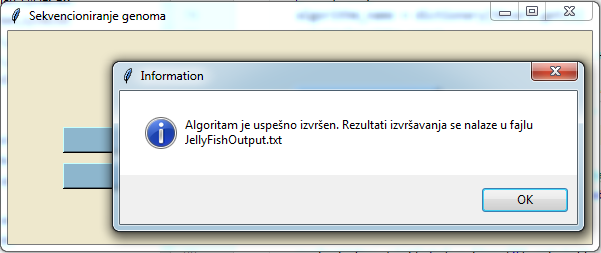
\includegraphics[width=\textwidth]{uspesan_algoritam.PNG}
\caption{Izbor algoritma}
\label{fig:uspesnoIzvrsavanje}
\end{figure}

Ukoliko je prilikom pokretanja algoritma detektovano nepoklapanje u izabranom algoritmu i ulaznom fajlu, pojaviće se upozorenje koje je prikazano na slici \ref{fig:neuspesnoIzvrsavanje}. U tom slučaju je potrebno proveriti izabrane vrednosti i ponovo pokrenuti algoritam.

\begin{figure}[h]
\centering
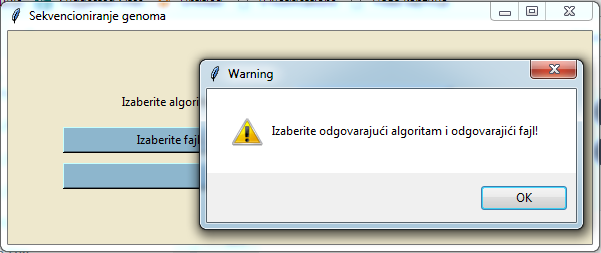
\includegraphics[width=\textwidth]{neuspesan_algoritam.PNG}
\caption{Izbor algoritma}
\label{fig:neuspesnoIzvrsavanje}
\end{figure}

\newpage

\subsection{Primeri upotrebe}

\textbf{Algoritam \textit{JellyFish}} - Ulazni fajl \textit{JellyFishData.txt} sadrži k-mere razdvojene zarezom i u poslednjoj liniji parametar alfa. Nakon izbora ovog ulaznog fajla i pokretanja algoritma \textit{JellyFish}, rezultat je smešten u tekstualnom fajlu \textit{jellyfish.txt}. Implementirane su dve varijante izvršavanja algoritma \textit{JellyFish} -- \textbf{sekvencijalna} i \textbf{paralelna}. U obe varijante ulazni fajl ima isti format i primer fajla koji sadrži k-mere dužine 2 može se videti na listingu \ref{lst:jellyfishUlazniFajl}.

\lstinputlisting[language=erlang,label={lst:jellyfishUlazniFajl},caption=Primer ulaznog fajla za algoritam \textit{JellyFish},captionpos=b]{jellyfish_ulazni_fajl.ex}

U sekvencijaloj varijanti algoritam se izvršava na celom skupu k-mera i rezultat je torka $\{H, Count\}$ čiji su elementi mapa $H$ i mapa $Count$. Rezultati se očitavaju tako što k-meru, koji je dodeljen ključu u prvoj mapi, odgovara broj pojavljivanja dodeljen istom ključu u drugoj mapi. Na listingu \ref{lst:jellyfishRezultatiSekvencijalno} se može videti sadržaj izlaznog fajla \textit{jellyfish.txt}.

\lstinputlisting[language=erlang,label={lst:jellyfishRezultatiSekvencijalno},caption=Rezultati sekvencijalnog izvršavanja algoritma \textit{JellyFish},captionpos=b]{jellyfishRezultati.ex}

U paralelnoj varijanti je omogućeno da se algoritam izvršava paralalno u okviru više procesa. Zapravo, početni skup k-mera je podeljen u onoliko skupova koliko računar ima procesora, a zatim je kreirano isto toliko procesa u okviru kojih je na tim skupovima izvršen algoritam \textit{JellyFish}. Rezultat je mapa čiji su ključevi jedinstveni k-meri iz polaznog skupa, a vrednosti su brojevi njihovog pojavljivanja u tom skupu i može se videti na listingu \ref{lst:jellyfishRezultatiParalelno}.

\lstinputlisting[language=erlang,label={lst:jellyfishRezultatiParalelno},caption=Rezultati paralelnog izvršavanja algoritma \textit{JellyFish},captionpos=b]{jellyfishRezultatiParalelno.ex}

Na malom skupu podataka, kakav je dat na listingu \ref{lst:jellyfishUlazniFajl}, nema mnogo smisla vršiti paralelizaciju izvršavanja. Primer gde ima smisla vršiti podelu ulaznog skupa podataka i paralelizovati izvršavanje biće dat u poglavlju \ref{odeljak:Rezultati}.

\textbf{Algoritam \textit{DSK}} - Ulazni fajl \textit{DSKData.txt} za algoritam \textit{DSK} ima isti format kao i ulazni fajl za algoritam \textit{JellyFish}, s tim što umesto parametra alfa u poslednje dve linije sadrži parametre $M$ i $D$. Primer ulaznog fajla može se videti na listingu \ref{lst:dskUlazniFajl}.

\lstinputlisting[language=erlang,label={lst:dskUlazniFajl},caption=Primer ulaznog fajla za algoritam \textit{DSK},captionpos=b]{dskUlazniFajl.ex}

Rezultati izvršavanja algoritma su smešteni u fajlu \textit{dsk.txt} i mogu se videti na listingu \ref{lst:dskRezultati}. Izlazni fajl se sastoji od lista u kojima se nalaze podliste. Nakon svake liste sledi prikaz najpre heš tabele $H$, a potom i prikaz tabele \textit{Count} za svaku od podlista.

\lstinputlisting[language=erlang,label={lst:dskRezultati},caption=Rezultati izvršavanja \textit{DSK} algoritma,captionpos=b]{dskRezultati.ex}

% Ušteda prostora u ovom algoritmu se ogleda u ograničavanju memorije koja će biti iskorišćena za smeštanje k-mera u liste i podliste, a sve to zahvaljujući parametrima $M$ i $D$. Ukoliko je parametar $D$ približno jednak broju $N$ k-mera u datom skupu k-mera, algoritam će biti izuzetno brz i izvršiće se u $O(kN)$ očekivanom vremenu.

\textbf{Algoritam \textit{DeBrujinGraph}} - Ulazni fajl \textit{DeBrujinData.txt} sadrži jedno očitavanje i u poslednjoj liniji parametar $k$. Primer ulaznog fajla sa očitavanjem dužine 17 i parametrom $k = 3$ može se videti na listingu \ref{lst:debrujinUlazniFajl}.

\lstinputlisting[language=erlang,label={lst:debrujinUlazniFajl},caption=Primer ulaznog fajla za algoritam \textit{DeBrujinGraph},captionpos=b]{debrujinUlazniFajl.ex}

Nakon izvršavanja algoritma \textit{DeBrujinGraph}, rezultat se može videti u tekstualnom fajlu \textit{deBrujinGraph.txt}, čiji prikaz se nalazi na listingu \ref{lst:debrujinRezultati}. Izlazni fajl sadrži mapu na osnovu koje se može konstruisati De Brojnov graf. Svaki ključ mape predstavlja čvor grafa, a lista njegovih vrednosti predstavlja čvorove sa kojima gradi granu.

\lstinputlisting[language=erlang,label={lst:debrujinRezultati},caption=Rezultati izvršavanja \textit{DeBrujinGraph} algoritma,captionpos=b]{debrujinRezultati.ex}

\textbf{Algoritam \textit{AllEulerianCycles}} - Ulazni fajl \textit{EulerData.txt} sadrži De Brojnov graf, koji je zapisan tako da elementi odvojeni sa $;$ predstavljaju jedan element mape, čiji je ključ k-mer sa leve strane znaka $:$, a vrednost lista k-mera koji se nalaze sa desne strane znaka $:$ i razdvojeni su zarezom. Primer ulaznog fajla može se videti na listingu \ref{lst:eulerUlazniFajl}.

\lstinputlisting[language=erlang,label={lst:eulerUlazniFajl},caption=Primer ulaznog fajla za algoritam \textit{AllEulerianCycles},captionpos=b]{allEulerianCyclesUlazniFajl.ex}

Nakon izvršavanja algoritma, rezultat je smešten u tekstualnom fajlu \textit{allEulerianCyceles.txt}. Izlazni fajl sadrži listu kontiga, koje predstavljaju cikluse u De Brojnovom grafu i prikazane su na listingu \ref{lst:eulerRezultati}.

\lstinputlisting[language=erlang,label={lst:eulerRezultati},caption=Rezultati izvršavanja \textit{AllEulerianCycles} algoritma,captionpos=b]{eulerRezultati.ex}

\newpage

\section{Rezultati}
\label{odeljak:Rezultati}

U ovom poglavlju će biti prikazani rezultati izvršavanja algoritama, koji su nakon toga smešteni u odgovarajućim tekstualnim fajlovima i mogu se upoređivati za različite ulazne vrednosti.

\subsection{Algoritam \textit{JellyFish}}
\label{pododeljak:jellyfish}

% Ulazni fajl \textit{JellyFishData.txt} za algoritam \textit{JellyFish} sadrži k-mere razdvojene zarezom i u poslednjoj liniji parametar alfa ($0.7$). Nakon izvršavanja algoritma, rezultat je smešten u tekstualnom fajlu \textit{jellyfish.txt}. Implementirane su dve varijante izvršavanja algoritma \textit{JellyFish} -- \textbf{sekvencijalna} i \textbf{paralelna}. 

% U sekvencijaloj varijanti algoritam se izvršava na celom skupu k-mera odjednom i rezultat je torka $\{H, Count\}$ čiji su elementi mapa $H$ i mapa $Count$. Rezultati se očitavaju tako što k-meru, koji je dodeljen ključu u prvoj mapi, odgovara broj pojavljivanja dodeljen istom ključu u drugoj mapi. Na listingu ... se može videti sadržaj izlaznog fajla \textit{jellyfish.txt}.

% \lstinputlisting[language=erlang,label={lst:jellyfishRezultati},caption=Rezultati izvršavanja \textit{JellyFish} algoritma,captionpos=b]{jellyfishRezultati.ex}

% U paralelnoj varijanti je omogućeno da se algoritam izvršava paralalno u okviru više procesa. Zapravo, početni skup k-mera je podeljen u onoliko skupova koliko računar ima procesora, a zatim je kreirano isto toliko procesa u okviru kojih je na tim skupovima izvršen algoritam \textit{JellyFish}. Rezultat je mapa čiji su ključevi jedinstveni k-meri iz polaznog skupa, a vrednosti su brojevi njihovog pojavljivanja u tom skupu.
% Rezultati ovakvog izvršavanja u se videti na listingu ...

% \lstinputlisting[language=erlang,label={lst:jellyfishRezultati},caption=Rezultati izvršavanja \textit{JellyFish} algoritma,captionpos=b]{jellyfishRezultati.ex}

% Na slici ... se može videti brzina izvršavanja algoritma \textit{JellyFish} u odnosu na broj k-mera u ulaznom fajlu i u odnosu na to da li se izvršava sekvencijalo ili paralelno.

%Sllika

% Broj kolizija u toku heširanja k-mera je manji, a algoritam je brži i efikasniji, ukoliko za parametar $\alpha$ važi $\alpha \leq 0.7$, tako da se brzina i efikasnost mogu uporediti pokretanjem algoritma za različito $\alpha$. Na malom skupu podataka, unapređenje u pogledu brzine i efikasnosti je zanemarljivo, ali prilikom izvršavanja nad velikim skupom podataka je od velikog značaja.

\subsection{Algoritam \textit{DSK}}

% Ulazni fajl \textit{DSKData.txt} za algoritam \textit{DSK} sadrži isti skup k-mera kao i ulazni fajl za algoritam \textit{JellyFish}. Poslednje dve linije sadrže parametre $M$ (6) i $D$ (5). Rezultati izvršavanja algoritma su smešteni u fajlu \textit{dsk.txt} i mogu se videti na listingu \ref{lst:dskRezultati}. Izlazni fajl se sastoji od lista u kojima se nalaze podliste. Nakon svake liste sledi prikaz najpre heš tabele $H$, a potom i prikaz tabele \textit{Count} za svaku od podlista.

% \lstinputlisting[language=erlang,label={lst:dskRezultati},caption=Rezultati izvršavanja \textit{DSK} algoritma,captionpos=b]{dskRezultati.ex}

% Ušteda prostora u ovom algoritmu se ogleda u ograničavanju memorije koja će biti iskorišćena za smeštanje k-mera u liste i podliste, a sve to zahvaljujući parametrima $M$ i $D$. Ukoliko je parametar $D$ približno jednak broju $N$ k-mera u datom skupu k-mera, algoritam će biti izuzetno brz i izvršiće se u $O(kN)$ očekivanom vremenu.

\subsection{Algoritam \textit{DeBrujinGraph}}
\label{odeljak:debrujinRezultati}

% Ulazni fajl \textit{DeBrujinData.txt} sadrži jedno očitavanje i u poslednjoj liniji parametar $k$ (3). Nakon pokretanja algoritma \textit{DeBrujinGraph}, rezultat se može videti u tekstualnom fajlu \textit{deBrujinGraph.txt}, čiji prikaz se nalazi na listingu \ref{lst:debrujinRezultati}.

% \lstinputlisting[language=erlang,label={lst:debrujinRezultati},caption=Rezultati izvršavanja \textit{DeBrujinGraph} algoritma,captionpos=b]{debrujinRezultati.ex}

% Izlazni fajl sadrži mapu na osnovu koje se može konstruisati De Brojnov graf. Svaki ključ mape predstavlja čvor grafa, a lista njegovih vrednosti predstavlja čvorove sa kojima gradi granu.

\subsection{Algoritam \textit{AllEulerianCycles}}

% Na listingu \ref{lst:debrujinRezultati} je prikazan graf koji je dobijen pokretanjem algoritma \textit{DeBrujinGraph} i on će biti iskorišćen kao ulazni parametar za algoritam \textit{AllEulerianCycles}. Dakle, ulazni fajl \textit{EulerData.txt} sadrži pomenuti De Brojnov graf, koji je zapisan tako da elementi odvojeni sa $;$ predstavljaju jedan element mape, čiji je ključ k-mer sa leve strane znaka $:$, a vrednost lista k-mera koji se nalaze sa desne strane znaka $:$ i razdvojeni su zarezom. Nakon izvršavanja algoritma, dobija se lista kontiga koja je prikazana na listingu \ref{lst:eulerRezultati}.

% \lstinputlisting[language=erlang,label={lst:eulerRezultati},caption=Rezultati izvršavanja \textit{AllEulerianCycles} algoritma,captionpos=b]{eulerRezultati.ex}

% ------------------------------------------------------------------------------
\chapter{Zaključak}
\label{poglavlje:Zaključak}

U ovom radu su prikazane osnove sintakse i semantike programskog jezika Elixir. On je iskorišćen za implementaciju algoritama u oblasti sekvencioniranja genoma. Sekvencioniranje genoma je proces otkrivanja sastava genoma i od izuzetnog je značaja za modernu dijagnostiku, a posebno za dijegnostiku rizika od naslednih bolesti. Na ovaj način je prikazana primena Elixir-a u rešavanju realnih problema bioinformatičke prirode.

Kako je Elixir funkcionalni programski jezik, on omogućava da razmišljamo u terminima funkcija koje transformišu podatke. To znači da sama transformacija nikada ne menja podatke, već svaka primena funkcije potencijalno stvara novu, svežiju verziju podataka. U okviru rada ova osobina je iskorišćena u implementaciji svakog algoritma, jer se svaka implementacija sastoji od velikog broja funkcija koje obavljaju neki celovit posao.  Zahvaljujući tome dobijen je koncizan k$\hat{o}$d, povećana je njegova čitljivost i programiranje je bilo brže. Dodatno, ova karakteristika smanjuje potrebu za mehanizmima za sinhronizaciju podataka, pa je implementacija konkurentnosti algoritma \textit{JellyFish} bila jednostavna i pouzdana. Konkurentnost je jedna od glavnih karakteristika Elixir-a. Stvaranje velikog broja procesa koje ne podrazumeva smanjivanje performansi mašine je značajno smanjilo vreme izvršavanja algoritma \textit{JellyFish}. Zahvaljujući jednostavnoj i modernoj sintaksi, koja je prirodna za čitanje, ovaj programski jezik se veoma brzo savladava i uči. To je pomoglo da se veoma brzo nakon upoznavanja sa osnovama sintakse i semantike počne sa implementacijom algoritama i postigne visoka produktivnost.

% Za potrebe ovog rada, algoritmi su testirani na manjem skupu podataka, te pun potencijal Elixir-a nije došao do izražaja. 
% Buduća unapređenja implementiranih algoritama i aplikacije mogla bi da obuhvate podršku za testiranje na realnim skupovima podataka, koji se inače u ovoj oblasti obrađuju. U pitanju su milijarde nukleotida od kojih se može sastojati jedan genom. U tom slučaju potrebno je izvršiti podelu posla i paralelizaciju izvršavanja. Polazni skup podataka bi se podelio na veliki broj manjih, a zatim bi se paralelno izvršili algoritmi na tim skupovima. Pojedinačni rezultati bi se sjedinili i na taj način formirali jedan krajnji rezultat. Na kraju bi se mogle uporedili brzine izvršavanja za ceo skup podataka i podeljene skupove. Tada bismo se još više uverili da je Elixir pravi izbor za ovu vrstu problema, kao i za sve ostale gde je potrebno obraditi ogromne količine podataka i gde su od presudnog značaja stabilnost, brzina i otpornost na greške prilikom obrade.
 


% ------------------------------------------------------------------------------
%\pangrami

.%\pangrami

% ------------------------------------------------------------------------------
% Literatura
% ------------------------------------------------------------------------------
\literatura

% ==============================================================================
% Završni deo teze i prilozi
\backmatter
% ==============================================================================

% ------------------------------------------------------------------------------
% Biografija kandidata
% \begin{biografija}
%   \textbf{Vuk Stefanović Karadžić} (\emph{Tršić,
%     26. oktobar/6. novembar 1787. — Beč, 7. februar 1864.}) bio je
%   srpski filolog, reformator srpskog jezika, sakupljač narodnih
%   umotvorina i pisac prvog rečnika srpskog jezika.  Vuk je
%   najznačajnija ličnost srpske književnosti prve polovine XIX
%   veka. Stekao je i nekoliko počasnih mastera.  Učestvovao je u
%   Prvom srpskom ustanku kao pisar i činovnik u Negotinskoj krajini, a
%   nakon sloma ustanka preselio se u Beč, 1813. godine. Tu je upoznao
%   Jerneja Kopitara, cenzora slovenskih knjiga, na čiji je podsticaj
%   krenuo u prikupljanje srpskih narodnih pesama, reformu ćirilice i
%   borbu za uvođenje narodnog jezika u srpsku književnost. Vukovim
%   reformama u srpski jezik je uveden fonetski pravopis, a srpski jezik
%   je potisnuo slavenosrpski jezik koji je u to vreme bio jezik
%   obrazovanih ljudi. Tako se kao najvažnije godine Vukove reforme
%   ističu 1818., 1836., 1839., 1847. i 1852.
% \end{biografija}
% ------------------------------------------------------------------------------

\end{document}